% This must be in the first 5 lines to tell arXiv to use pdfLaTeX, which is strongly recommended.
\pdfoutput=1
% In particular, the hyperref package requires pdfLaTeX in order to break URLs across lines.

\documentclass[11pt]{article}

% Remove the "review" option to generate the final version.
%\usepackage[review]{acl}
\usepackage{acl}

% Standard package includes
\usepackage{times}
\usepackage{latexsym}

% For proper rendering and hyphenation of words containing Latin characters (including in bib files)
\usepackage[T1]{fontenc}
% For Vietnamese characters
% \usepackage[T5]{fontenc}
% See https://www.latex-project.org/help/documentation/encguide.pdf for other character sets

% This assumes your files are encoded as UTF8
\usepackage[utf8]{inputenc}

% This is not strictly necessary, and may be commented out,
% but it will improve the layout of the manuscript,
% and will typically save some space.
\usepackage{microtype}

% If the title and author information does not fit in the area allocated, uncomment the following
%
%\setlength\titlebox{<dim>}
%
% and set <dim> to something 5cm or larger.

\title{InstructEval: Systematic Evaluation of Instruction Selection Methods}

% Author information can be set in various styles:
% For several authors from the same institution:
% \author{Author 1 \and ... \and Author n \\
%         Address line \\ ... \\ Address line}
% if the names do not fit well on one line use
%         Author 1 \\ {\bf Author 2} \\ ... \\ {\bf Author n} \\
% For authors from different institutions:
% \author{Author 1 \\ Address line \\  ... \\ Address line
%         \And  ... \And
%         Author n \\ Address line \\ ... \\ Address line}
% To start a seperate ``row'' of authors use \AND, as in
% \author{Author 1 \\ Address line \\  ... \\ Address line
%         \AND
%         Author 2 \\ Address line \\ ... \\ Address line \And
%         Author 3 \\ Address line \\ ... \\ Address line}

\author{Anirudh Ajith$^{*}$ \quad Chris Pan$^{*}$\quad Mengzhou Xia \quad Ameet Deshpande \quad Karthik Narasimhan \\
\textnormal{Department of Computer Science, Princeton University} \\
\texttt{\{anirudh.ajith, chrispan, mengzhou, asd, karthikn\}@princeton.edu}
}

%%%%% Packages %%%%%
\usepackage{amsmath,amsfonts}
\usepackage{booktabs,arydshln}
\usepackage{multirow}
\usepackage{ulem}
\usepackage{pifont}
\usepackage{relsize}
\usepackage{enumitem}
\usepackage{graphicx}
\usepackage{amssymb}% http://ctan.org/pkg/amssymb
\usepackage{pifont}% http://ctan.org/pkg/pifont
\usepackage{dcolumn}
\usepackage{xcolor,colortbl}
\usepackage{supertabular}
\usepackage{tikz}
\usepackage{subcaption}
\usepackage{svg}
\usepackage{float}
\restylefloat{table}
\usepackage{enumitem}



%\usepackage[sfdefault,light]{FiraSans}
% \usepackage{minted}
% \usepackage[dvipsnames]{xcolor}

\newcolumntype{d}[1]{D{.}{.}{#1}}  % `d' column type aligns at decimal point

%%%%% Commands %%%%%
\newcommand{\cmark}{\ding{51}}%
\newcommand{\xmark}{\ding{55}}%
\newcommand{\greyrule}{\arrayrulecolor{black!30}\midrule\arrayrulecolor{black}}

%%%%%%%% Command for dashed lines %%%%%%%%
\makeatletter
\def\adl@drawiv#1#2#3{%
        \hskip.5\tabcolsep
        \xleaders#3{#2.5\@tempdimb #1{1}#2.5\@tempdimb}%
                #2\z@ plus1fil minus1fil\relax
        \hskip.5\tabcolsep}
\newcommand{\cdashlinelr}[1]{%
  \noalign{\vskip\aboverulesep
           \global\let\@dashdrawstore\adl@draw
           \global\let\adl@draw\adl@drawiv}
  \cdashline{#1}
  \noalign{\global\let\adl@draw\@dashdrawstore
           \vskip\belowrulesep}}
\makeatother


%%%%%%%% Review %%%%%%%%

\newcommand{\draftonly}[1]{#1} % uncomment to remove comments
\newcommand{\draftcomment}[3]{\draftonly{{\color{#2}{{{[#1: #3]}}}}}}
\newcommand{\anirudh}[1]{\draftcomment{Anirudh}{blue}{#1}}
\newcommand{\chris}[1]{\draftcomment{Chris}{teal}{#1}}
\newcommand{\ameet}[1]{\draftcomment{Ameet}{orange}{#1}}
\newcommand{\mz}[1]{\draftcomment{Mengzhou}{green}{#1}}
\newcommand{\karthik}[1]{\draftcomment{Karthik}{brown}{#1}}

%%%%%%%% Reference %%%%%%%%
\newcommand{\secref}[1]{Section~\ref{#1}}
\newcommand{\symbolsecref}[1]{($\S$~\ref{#1})}
\newcommand{\tableref}[1]{Table~\ref{#1}}
\newcommand{\figref}[1]{Figure~\ref{#1}}

\usetikzlibrary{backgrounds, shapes,arrows,positioning,matrix,fit}

\definecolor{lightblue}{RGB}{173,216,230}
\definecolor{lightpink}{RGB}{255,182,193}
\definecolor{lightyellow}{rgb}{0.9,0.9,0.6}
\definecolor{darkyellow}{rgb}{0.7, 0.7, 0.3}

\newcommand{\normalFont}[1]{\fontseries{m}\selectfont#1\fontseries{m}\selectfont}
\newcommand{\ultraLight}[1]{\fontseries{l}\selectfont#1\fontseries{m}\selectfont}

\pgfdeclarelayer{main}
\pgfdeclarelayer{layer1}
\pgfdeclarelayer{layer2}
\pgfdeclarelayer{layer3}
\pgfdeclarelayer{layer4}
\pgfdeclarelayer{layer5}
\pgfdeclarelayer{layer6}
\pgfsetlayers{layer6, layer5,layer4,layer3, layer2, layer1, main}


\begin{document}
\maketitle
\renewcommand{\thefootnote}{\fnsymbol{footnote}}
\footnotetext[1]{Equal contribution}
\renewcommand{\thefootnote}{\arabic{footnote}}

\begin{abstract}
\label{sec:abstract}

%% 1. what is the problem 
Scientific applications that run on leadership computing facilities often face the challenge 
of being unable to fit leading science cases onto accelerator devices due to memory constraints 
(memory-bound applications).
%
% 2. what is your solution 
In this work, the authors studied one such US Department of Energy mission-critical condensed matter 
physics application, Dynamical Cluster Approximation (DCA++), and this paper discusses how device memory-bound challenges were successfully reduced  by proposing an effective 
``all-to-all'' communication method---a ring communication algorithm. 
%
This implementation takes advantage of acceleration on GPUs and remote direct memory access (RDMA) for fast data exchange between GPUs. 
%
\\Additionally, the ring algorithm was optimized with sub-ring communicators
and multi-threaded support to further reduce communication overhead and 
expose more concurrency, respectively.
%
% 3. What's the cherry-picked evaluation result you want to mention
The computation and communication were also analyzed 
by using the Autonomic Performance Environment for Exascale 
(APEX) profiling tool,  and this paper further discusses the 
performance trade-off for the ring algorithm implementation. 
%
The memory analysis on the ring algorithm shows that the allocation size for the authors' most 
memory-intensive data structure per GPU is now reduced to $1/p$ of the original size, where $p$ is the number of GPUs in the ring communicator.
%
The communication analysis suggests that 
the distributed Quantum Monte Carlo execution time grows linearly as sub-ring size increases, and the cost of messages passing through the network interface connector could be a limiting factor.


%
% \todoRed{Ronnie: Next sentence needs rewrite, too much information about Green's function that no one knows in the abstract; recommend generalizing.} \emph {However, DCA++ is currently facing memory-bound challenge as 
% a larger device array $G_t$ is limited by device memory size, where
% $G_t$ is a two-particle Green's function that allows condensed matter
% scientists to explore larger and more complex (higher fidelity)
% physics cases.}

\end{abstract}

\keywords{DCA++, Quantum Monte Carlo, GPU Remote Direct Memory Access, memory-bound issue, exascale machines}

\section{Introduction}  \label{sec:introduction}

\newcommand\inexpIntro[3]{#1?(#2,#3).}
\newcommand\rinexpIntro[3]{*#1?(#2,#3).}
\newcommand\outexpIntro[3]{#1!(#2,#3).}
\newcommand\outatomIntro[3]{#1!(#2,#3)}

We propose a fully automated method for proving termination of \(\pi\)-calculus processes.
Although there have been a lot of studies on termination analysis for the \(\pi\)-calculus
and related calculi~\cite{Deng06IC,Demangeon07,SangiorgiTermination,KobayashiHybrid,Yoshida04IC,DBLP:journals/jlp/DemangeonHS10,Venet98SAS}, most of them have been rather theoretical,
and there have been surprisingly little efforts in developing  fully automated termination
verification methods and tools based on them. To our knowledge,
Kobayashi's \typical{}~\cite{TyPiCal,KobayashiHybrid} is the only exception that
can prove termination of \(\pi\)-calculus processes (extended with natural numbers)
fully automatically, but its termination analysis is quite limited (see Section~\ref{sec:relatedwork}).

Our method is based on a reduction to termination analysis for sequential programs:
we translate a \(\pi\)-calculus process \(P\) to a sequential program \(S_P\), so that
if \(S_P\) is terminating, so is \(P\). The reduction allows us to use
powerful, mature methods and tools
for termination analysis of sequential programs~\cite{heizmann2016ultimate,freqterm,DBLP:conf/lics/PodelskiR04,Kuwahara2014Termination,DBLP:journals/cacm/CookPR11}.

The idea of the translation is to convert a chain of communications on replicated input
channels to a chain of recursive function calls of the target sequential program.
Let us consider the following Fibonacci process:
\begin{align*}
    & \rinexpIntro{\fib}{n}{r}
        \ifexp{n<2}{ \soutatom{r}{1} \\ &\quad}
                   { \nuexp{s_1} \nuexp{s_2} (\outatomIntro{\fib}{n-1}{s_1} \PAR \outatomIntro{\fib}{n-2}{s_2} \PAR \sinexp{s_1}{x}\sinexp{s_2}{y}\soutatom{r}{x+y}) \\}
    & \PAR \outatomIntro{\fib}{m}{r}
\end{align*}
Here, the process
$\rinexpIntro{\fib}{n}{r} \ldots$ is a function server that computes the \(n\)-th Fibonacci number
in parallel and returns the result to \(r\),
and $\outatom{\fib}{m}{r}$ sends a request for computing the \(m\)-th Fibonacci number;
those who are not familiar with the syntax of the \(\pi\)-calculus may wish to consult
Section~\ref{sec:targetlanguage} first.
To prove that the process above is terminating for any integer \(m\),
it suffices to show that there is no infinite chain of communications on $\fib$:
\[
    \fib(m,r) \to \fib(m_1,r_1) \to \fib(m_2,r_2) \to \cdots.
\]
We convert the process above to the following program:\footnote{The actual translation
  given later is a little more complex.}
\begin{verbatim}
 let rec fib(n) = if n<2 then () else (fib(n-1) [] fib(n-2)) in
 fib(m)
\end{verbatim}
Here, \texttt{[]} represents the non-deterministic choice.
Note that, although the calculation of Fibonacci numbers is not preserved,
for each chain of communications on \texttt{fib}, there is a corresponding
sequence of recursive calls:
\[
\mathtt{fib}(m) \to \mathtt{fib}(m_1) \to \mathtt{fib}(m_2) \to \cdots.
\]
Thus, the termination of the sequential program above implies the termination of
the original process.
As shown in the example above, (i) each communication on a replicated input channel
is converted to a function call, (ii) each communication on a non-replicated input
channel is just removed (or, in the actual translation, replaced by a call of
a trivial function defined by \(f(\seq{x})=(\,)\)), and (iii) parallel composition
is replaced by a non-deterministic choice.
We formalize the translation outlined above and prove its correctness.

The basic translation sketched above sometimes loses too much information.
For example, consider the following process:
\begin{align*}
    & \rinexpIntro{\pre}{n}{r} \soutatom{r}{n-1} \\
    & \PAR \rinexpIntro{f}{n}{r} \ifexp{n<0}{ \soutatom{r}{1} }
                                       { \nuexp{s} (\outatomIntro{\pre}{n}{s} \PAR \sinexp{s}{x}\outatomIntro{f}{x}{r}) } \\
    & \PAR \outatomIntro{f}{m}{r}
\end{align*}
The translation sketched above would yield:
\begin{verbatim}
  let pred(n) = n-1 in
  let rec f(n) = if n<0 then () else (pred(n) [] f(*)) in
  f(m)
\end{verbatim}
Here, \texttt{*} represents a non-deterministic integer: since we have removed
the input $\sinatom{s}{x}$, we do not have information about the value of \( x \).
As a result, the sequential program above is non-terminating, although the original
process is terminating.
To remedy this problem, we also refine the basic translation above by using a refinement
type system for the \(\pi\)-calculus. Using the refinement type system,
we can infer that the value of \(x\) in the original process is less than \(n\),
so that we can refine the definition of \texttt{f} to:
\begin{verbatim}
 let rec f(n) = ... else (pred(n) [] let x=* in assume(x<n);f(x))
\end{verbatim}
The target program is now terminating, from which
we can deduce that the original process is also terminating.
We have implemented an automated tool based on the refined translation above.

The contributions of this paper are summarized as follows.
\begin{itemize}
\item The formalization of the basic translation from the \(\pi\)-calculus
  (extended with integers) to sequential programs, and a proof of its correctness.
\item The formalization of a refined translation based on a refinement type system.
\item An implementation of the refined translation, including automated refinement type
  inference based on CHC solving, and experiments to evaluate the effectiveness of
  our method.
\end{itemize}

The rest of this paper is structured as follows.
Section~\ref{sec:targetlanguage} introduces the source and target languages
of our translation.
Section~\ref{sec:approach} 
formalizes the basic translation, and proves its correctness.
Section~\ref{sec:refinement} refines the basic translation by using a refinement type system.
Section~\ref{sec:implementation} reports an implementation and experiments.
Section~\ref{sec:relatedwork} discusses related work,
and Section~\ref{sec:conclusion} concludes the paper.

The industry standard for pose edition is to create rigs, a collection of pieces of software designed to manipulate a character's skeleton. The rig describes the skeleton's bones, how they relate to each other, are constrained in their possible motion and are deformed. These rules are loosely specified and creating a good rig requires a detailed understanding of physics and anatomy, as well as technical and artistic skills. Rigging is thus a time consuming task even for experienced animators, and even more so in large scale productions which often require a different in-depth rig for each character in the cast.
Previous work has helped alleviate this difficulty by providing efficient tools to speed up/and or ease the rigging process, relying on inverse kinematics or data-driven methods.
\subsection{Character pose design}
\subsubsection{Inverse Kinematics (IK)}
IK solvers are a family of methods commonly used in robotics, engineering and computer graphics, in which the parameterization of a kinematic chain is determined from the position of its end effector.
They are a staple tool in pose design software, ensuring the respect of elementary constraints during pose edition. Their de-facto role is to guarantee the length of the limbs, and in some cases to enforce the orientation angle range of a joint.
Many IK solutions have been studied over the years \cite{aristidou_inverse_2018}; usually revolving around approximated linearizations or heuristics. 

Numerical methods require a set of iterations to achieve a satisfactory solution formulated by a cost function to be minimized.
IK solutions can generally be divided into three sub-categories: Jacobian \cite{Siciliano_Handbook_Robot_2007}, Newtonians \cite{cohen_ik_1996} and Heuristics. Most software implement heuristic methods such as Cyclic Coordinate Descent (CCD) \cite{wang_ccd_1991} or 
Forward-Backward Reaching IK (FABRIK) \cite{aristidou_fabrik:_2011} due to their simplicity and extensibility. 

The main drawback of 
these solvers is that they manipulate kinematic chains without taking into account many morphological aspects that make a pose more or less plausible. They offer a first level of help to users but are not sufficient to guarantee a realistic pose. Many joints constraints are dependent on each other and require subjective, human-made approximations.

\subsubsection{Data-driven pose edition}
Data-driven methods offer promising opportunities to solve these approximations. Using real-life data can help in modelling the complex inter-dependencies of skeletons and providing users with smarter edition tools.
While it is still an early field of research, some solutions have been studied. Wu \etal \cite{wu_posing_2009} propose a method for natural character posing from a large motion database. It employs adaptive KD-clustering to select a representative frame from a database and sparse approximations to accelerate training and posing. 
Huang \etal in \cite{Huang_IK_MGDM_2017} present a method based on the formulation of multi-variate Gaussian distribution models (MGDMs), which learn the joint constraints of a kinematic skeleton from motion capture data. 

Some work has also been dedicated to finding new editing interfaces. \modify{}{Instead of the usual setup manipulating joints directly, Guay \etal \cite{guay_line_2013} articulate a framework based on the conceptual "line of action" which describes the overall pose dynamics. They provide a mathematical definition of the line of action, and a interface in which the software modifies the pose to follow a user-provided line. In the same line of though} Garcia \etal \cite{garcia_sketching_2019} propose \modify{a method transforming doodle of trajectories (position and orientation over time) }{a virtual reality-based interface where the user's hands motion (position and orientation over time) are transformed} into sequences of actions and then into detailed character animations using a dataset of parametrized motion clips automatically fitted to the trajectory. 

% ==> DL et Latent Space. 
\subsection{Neural modelling of human motion}
Neural networks have received a great amount of attention over the last decade and shown impressive result in modelling complex data. Human motion has not been spared and deep learning methods have proven their capability of generating realistic motion in a number of difficult cases. 

The literature in neural-based animation include example in user-controlled character navigation \cite{Holden2017} and interactions with the environment \cite{starke_neural_2019}. 
Holden \etal \cite{Holden2020} also show that neural networks can be used to replace parts of existing data-driven methods, improving their scalability potential.
More recently, some work has also focused on improving smaller parts of the animation pipeline rather than replacing it completely. Berson et al. \cite{berson_intuitive_2020} leverage neural networks to provide an interactive system to edit facial animation. 

% Wrap up
Data-driven IK and pose editing can relieve animators from time-consuming, back-and-forth pose adjustments by applying constraints extracted from real-world data. Recently, neural-network-based approaches have demonstrated their ability to model the intricacies of human motion while scaling to large amount of data and retaining a fast inference time. In this paper we seek to take advantage of these properties to create an efficient posing tool, intuitively usable even by a inexperienced user.
\section{Evaluation Suite}
%We design a comprehensive evaluation suite to assess the performance of instructions along 5 metrics relevant to practical ICL. To ensure a fair analysis, we test each instruction selection method across 9 tasks and 13 autoregressive models from 4 model families.

\subsection{Prompt format}

\begin{figure}[t]
    \centering
    %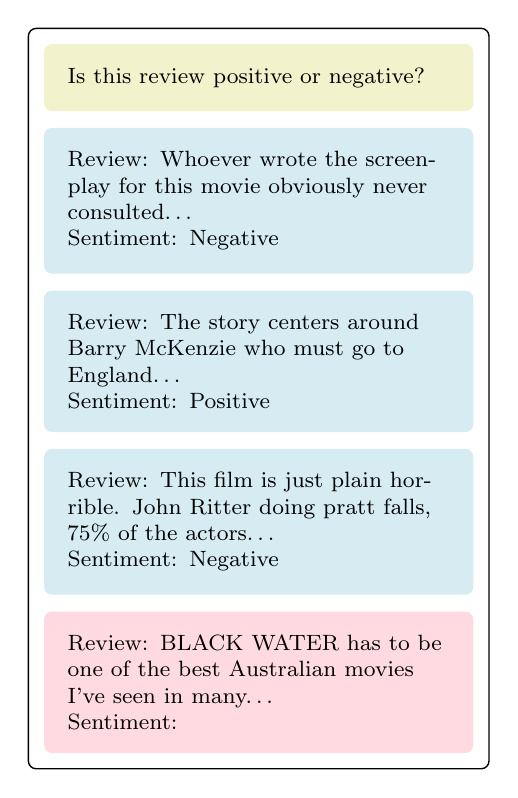
\begin{tikzpicture}[
  node distance = 0.2cm and 0.2cm,
  single node/.style = {rectangle, fill=#1, fill opacity=0.5, text opacity=1, align=left, font=\fontfamily{FiraSans-LF}\selectfont\footnotesize, text width=0.40\textwidth, inner xsep=3mm, inner ysep=3mm, rounded corners=1mm},
]

\node[single node=lightyellow] (instruction) 
{\normalFont{Is this review positive or negative?}};

\node[single node=lightblue, below=of instruction] (example1)
{\normalFont{Review:} \ultraLight{Whoever wrote the screenplay for this movie obviously never consulted…} \\ \normalFont{Sentiment:} \ultraLight{Negative}};

\node[single node=lightblue, below=of example1] (example2)
{\normalFont{Review:} \ultraLight{The story centers around Barry McKenzie who must go to England…} \\ \normalFont{Sentiment:} \ultraLight{Positive}};

\node[single node=lightblue, below=of example2] (example3)
{\normalFont{Review:} \ultraLight{This film is just plain horrible. John Ritter doing pratt falls, 75\% of the actors…} \\ \normalFont{Sentiment:} \ultraLight{Negative}};


\node[single node=lightpink, below=of example3] (test) 
{\normalFont{Review:} \ultraLight{BLACK WATER has to be one of the best Australian movies I've seen in many…} \\ \normalFont{Sentiment:} };

\draw [black, line width=0.5pt, rounded corners=1mm] ([shift={(-2mm,-2mm)}]current bounding box.south west) rectangle ([shift={(2mm,2mm)}]current bounding box.north east);

\end{tikzpicture}
    \includegraphics[width=\linewidth]{figures/prompt_example.png}
    \caption{
        An example of a prompt following the template we use for IMDB. By  `prompt' we refer to the concatenation of the \textcolor{darkyellow}{instruction}, solved \textcolor{blue}{demonstrations} and an unsolved \textcolor{red}{test example}.
    }
    \label{fig:prompt_example}
\end{figure}
We define a `prompt' as the full textual input provided to an LLM. Our evaluation suite supports the use of any number of demonstrations, arbitrary demonstration templates and the inclusion of custom strings anywhere within the prompt. Since the instructions used can be set to any arbitrary strings, users are free to use any external means to select instructions and have them evaluated by our suite.

For consistency, we conduct all experiments in this work using prompts that begin with an instruction, continue with a sequence of annotated training demonstrations, and conclude with an unsolved test example\footnote{Instructions are omitted during `Null instruction' evaluations. Demonstrations are omitted in zero-shot evaluations.} (Figure~\ref{fig:prompt_example}), and express each example in a minimal, task-specific key-value format (Table~\ref{table:templates}) that reflects task semantics.

\subsection{Metrics}
\begin{figure*}
  \begin{subfigure}[b]{0.32\textwidth}
    \centering
    \resizebox{\linewidth}{!}{
    \iffalse

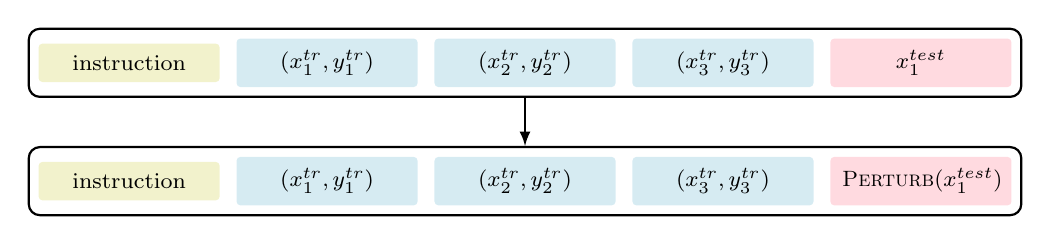
\begin{tikzpicture}[
  node distance = 0.2cm and 0.2cm,
  single node/.style = {rectangle, fill=#1, text opacity=1, opacity=0.5, align=center, font=\footnotesize, text width=2cm, inner sep=1.5mm, rounded corners=0.5mm},
  bigbox/.style = {draw, thick, rounded corners, rectangle},
  arrow/.style={thick, -latex},
]

\node[single node=lightyellow] (instruction) {instruction};

\node[single node=lightblue, right=of instruction] (example1) {$(x_1^{tr}, y_1^{tr})$};
\node[single node=lightblue, right=of example1] (example2) {$(x_2^{tr}, y_2^{tr})$};
\node[single node=lightblue, right=of example2] (example3) {$(x_3^{tr}, y_3^{tr})$};

\node[single node=lightpink, right=of example3] (test) {$x_1^{test}$};

\node[bigbox, fit=(instruction) (example1) (example2) (example3) (test)] (box1) {};

\node[single node=lightyellow, below=1cm of instruction] (instruction2) {instruction};

\node[single node=lightblue, right=of instruction2] (example12) {$(x_1^{tr}, y_1^{tr})$};
\node[single node=lightblue, right=of example12] (example22) {$(x_2^{tr}, y_2^{tr})$};
\node[single node=lightblue, right=of example22] (example32) {$(x_3^{tr}, y_3^{tr})$};

\node[single node=lightpink, right=of example32] (test2) {\textsc{Perturb}$(x_1^{test})$};

\node[bigbox, fit=(instruction2) (example12) (example22) (example32) (test2)] (box2) {};

\draw [arrow] (box1.south) -- (box2.north);

\end{tikzpicture}

\fi


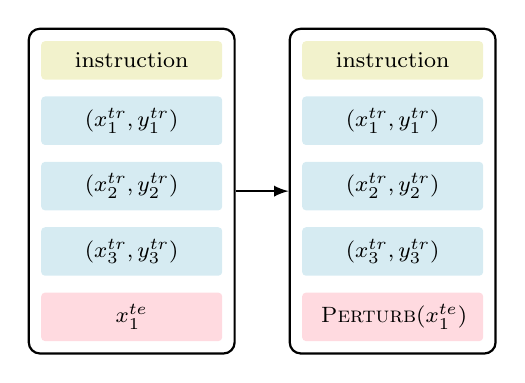
\begin{tikzpicture}[
  node distance = 0.2cm and 1cm, % Increase horizontal distance between nodes
  single node/.style = {rectangle, fill=#1, text opacity=1, opacity=0.5, align=center, font=\footnotesize, text width=2cm, inner sep=1.5mm, rounded corners=0.5mm},
  bigbox/.style = {draw, thick, rounded corners, rectangle, inner sep=1.5mm}, % Reduce inner sep for less padding
  arrow/.style={thick, -latex},
]

\node[single node=lightyellow] (instruction1) {instruction};
\node[single node=lightblue, below=of instruction1] (example1) {$(x_1^{tr}, y_1^{tr})$};
\node[single node=lightblue, below=of example1] (example2) {$(x_2^{tr}, y_2^{tr})$};
\node[single node=lightblue, below=of example2] (example3) {$(x_3^{tr}, y_3^{tr})$};
\node[single node=lightpink, below=of example3] (test1) {$x_1^{te}$};

\node[bigbox, fit=(instruction1) (example1) (example2) (example3) (test1)] (box1) {};

\node[single node=lightyellow, right=of instruction1] (instruction2) {instruction};
\node[single node=lightblue, below=of instruction2] (example12) {$(x_1^{tr}, y_1^{tr})$};
\node[single node=lightblue, below=of example12] (example22) {$(x_2^{tr}, y_2^{tr})$};
\node[single node=lightblue, below=of example22] (example32) {$(x_3^{tr}, y_3^{tr})$};
\node[single node=lightpink, below=of example32] (test2) {\textsc{Perturb}$(x_1^{te})$};

\node[bigbox, fit=(instruction2) (example12) (example22) (example32) (test2)] (box2) {};

\draw [arrow] (box1.east) -- (box2.west);
\end{tikzpicture}

    }
    \caption{Perturbation accuracy}
  \end{subfigure}\hfill
  \begin{subfigure}[b]{0.32\textwidth}
    \centering
    \resizebox{\linewidth}{!}{
    \input{figures/selection_example_tikz}
    }
    \caption{Selectional sensitivity}
  \end{subfigure}\hfill
  \begin{subfigure}[b]{0.32\textwidth}
    \centering
    \resizebox{\linewidth}{!}{
    \iffalse
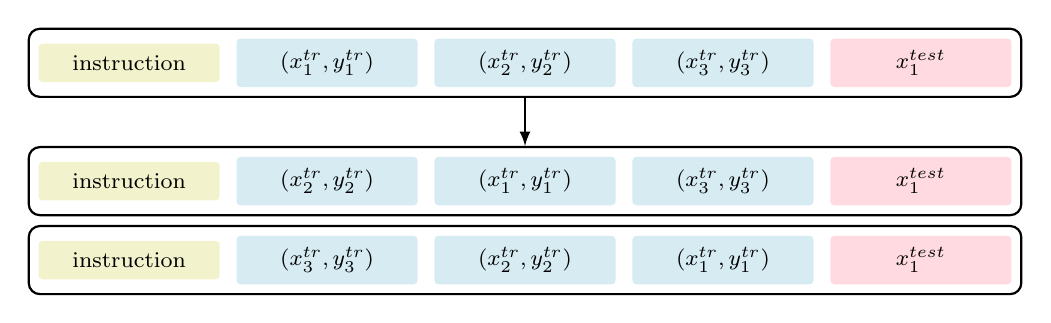
\begin{tikzpicture}[
  node distance = 0.2cm and 0.2cm,
  single node/.style = {rectangle, fill=#1, text opacity=1, opacity=0.5, align=center, font=\footnotesize, text width=2cm, inner sep=1.5mm, rounded corners=0.5mm},
  bigbox/.style = {draw, thick, rounded corners, rectangle},
  arrow/.style={thick, -latex},
]

\node[single node=lightyellow] (instruction) {instruction};

\node[single node=lightblue, right=of instruction] (example1) {$(x_1^{tr}, y_1^{tr})$};
\node[single node=lightblue, right=of example1] (example2) {$(x_2^{tr}, y_2^{tr})$};
\node[single node=lightblue, right=of example2] (example3) {$(x_3^{tr}, y_3^{tr})$};

\node[single node=lightpink, right=of example3] (test) {$x_1^{test}$};

\node[bigbox, fit=(instruction) (example1) (example2) (example3) (test)] (box1) {};

\node[single node=lightyellow, below=1cm of instruction] (instruction2) {instruction};

\node[single node=lightblue, right=of instruction2] (example12) {$(x_2^{tr}, y_2^{tr})$};
\node[single node=lightblue, right=of example12] (example22) {$(x_1^{tr}, y_1^{tr})$};
\node[single node=lightblue, right=of example22] (example32) {$(x_3^{tr}, y_3^{tr})$};

\node[single node=lightpink, right=of example32] (test2) {$x_1^{test}$};

\node[bigbox, fit=(instruction2) (example12) (example22) (example32) (test2)] (box2) {};

\draw [arrow] (box1.south) -- (box2.north);

\node[single node=lightyellow, below=0.5cm of instruction2] (instruction3) {instruction};

\node[single node=lightblue, right=of instruction3] (example13) {$(x_3^{tr}, y_3^{tr})$};
\node[single node=lightblue, right=of example13] (example23) {$(x_2^{tr}, y_2^{tr})$};
\node[single node=lightblue, right=of example23] (example33) {$(x_1^{tr}, y_1^{tr})$};

\node[single node=lightpink, right=of example33] (test3) {$x_1^{test}$};

\node[bigbox, fit=(instruction3) (example13) (example23) (example33) (test3)] (box3) {};


\end{tikzpicture}
\fi



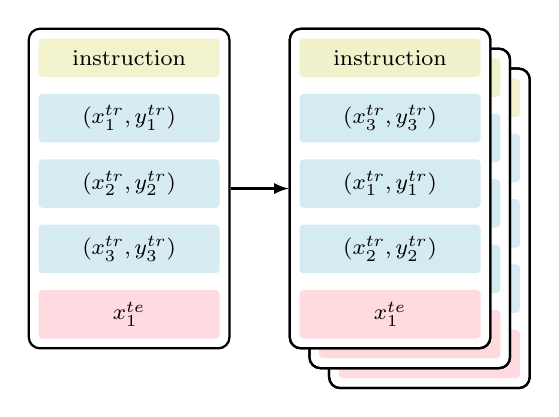
\begin{tikzpicture}[
  node distance = 0.2cm and 0.2cm,
  single node/.style = {rectangle, fill=#1, text opacity=1, opacity=0.5, align=center, font=\footnotesize, text width=2cm, inner sep=1.5mm, rounded corners=0.5mm},
  bigbox/.style = {draw, thick, rounded corners, rectangle},
  arrow/.style={thick, -latex},
  bigbox opaque/.style = {draw, thick, rounded corners, rectangle, opacity=1, fill=white},
  arrow/.style={thick, -latex},
]

\node[single node=lightyellow] (instruction) {instruction};

\node[single node=lightblue, below=of instruction] (example1) {$(x_1^{tr}, y_1^{tr})$};
\node[single node=lightblue, below=of example1] (example2) {$(x_2^{tr}, y_2^{tr})$};
\node[single node=lightblue, below=of example2] (example3) {$(x_3^{tr}, y_3^{tr})$};

\node[single node=lightpink, below=of example3] (test) {$x_1^{te}$};

\node[bigbox, fit=(instruction) (example1) (example2) (example3) (test)] (box1) {};

\begin{pgfonlayer}{layer1}
\node[single node=lightyellow, right=1cm of instruction] (instruction2) {instruction};

\node[single node=lightblue, below=of instruction2] (example12) {$(x_3^{tr}, y_3^{tr})$};
\node[single node=lightblue, below=of example12] (example22) {$(x_1^{tr}, y_1^{tr})$};
\node[single node=lightblue, below=of example22] (example32) {$(x_2^{tr}, y_2^{tr})$};

\node[single node=lightpink, below=of example32] (test2) {$x_1^{te}$};

\node[bigbox, fit=(instruction2) (example12) (example22) (example32) (test2)] (box2) {};
\end{pgfonlayer}

\begin{pgfonlayer}{layer2}
\node[bigbox opaque, fit=(instruction2) (example12) (example22) (example32) (test2)] (box2) {};
\end{pgfonlayer}

\begin{pgfonlayer}{layer3}
\node[single node=lightyellow, below=-0.25cm of instruction2, xshift=0.25cm] (instruction3) {instruction};

\node[single node=lightblue, below=of instruction3] (example13) {$(x_1^{tr}, y_1^{tr})$};
\node[single node=lightblue, below=of example13] (example23) {$(x_2^{tr}, y_2^{tr})$};
\node[single node=lightblue, below=of example23] (example33) {$(x_3^{tr}, y_3^{tr})$};

\node[single node=lightpink, below=of example33] (test3) {$x_1^{test}$};

\node[bigbox, fit=(instruction3) (example13) (example23) (example33) (test3)] (box3) {};
\end{pgfonlayer}

\begin{pgfonlayer}{layer4}
\node[bigbox opaque, fit=(instruction3) (example13) (example23) (example33) (test3)] (box3) {};
\end{pgfonlayer}

\begin{pgfonlayer}{layer5}
\node[single node=lightyellow, below=-0.25cm of instruction3, xshift=0.25cm] (instruction4) {instruction};

\node[single node=lightblue, below=of instruction4] (example14) {$(x_1^{tr}, y_1^{tr})$};
\node[single node=lightblue, below=of example14] (example24) {$(x_2^{tr}, y_2^{tr})$};
\node[single node=lightblue, below=of example24] (example34) {$(x_3^{tr}, y_3^{tr})$};

\node[single node=lightpink, below=of example34] (test4) {$x_1^{test}$};

\node[bigbox, fit=(instruction4) (example14) (example24) (example34) (test4)] (box4) {};
\end{pgfonlayer}

\begin{pgfonlayer}{layer6}
\node[bigbox, fit=(instruction4) (example14) (example24) (example34) (test4)] (box4) {};
\end{pgfonlayer}

\draw [arrow] (box1.east) -- (box2.west);

\end{tikzpicture}
    }
    \caption{Permutational sensitivity}
  \end{subfigure}
  \caption{
        We provide schematic diagrams that show prompts are modified to measure \textit{perturbation accuracy}, \textit{selectional sensitivity} and \textit{permutational sensitivity}. We perturb the test input to measure perturbation accuracy, and demonstration selection and permutation respectively while measuring selectional and permutational sensitivity.
    }
    \label{fig:sensitivity-metrics}
\end{figure*}

\label{sec:metrics}
\paragraph{Accuracy metrics} Accuracy is typically the primary metric of interest in ICL. While ICL is most commonly performed in few-shot settings where a handful of annotated demonstrations are included in the prompt, models are also prompted zero-shot without the use of such demonstrations. Since real-world scenarios can often contain grammatical errors and misspellings in the test input, it is desirable to find prompts robust to these perturbations. Hence, we measure \textit{zero-shot accuracy}, \textit{few-shot accuracy}, and \textit{perturbation accuracy}\footnote{We choose to treat this as an accuracy metric rather than a sensitivity metric since it is not meaningful to measure sensitivity to such perturbations in situations where a prompt only elicits near random-chance task performance from a model.} in our evaluations. Following \citet{helm}, we measure perturbation accuracy by introducing random capitalization, spacing, contractions and common misspellings in the test input.

\paragraph{Sensitivity metrics} Previous work has shown that the accuracy obtained using a prompt template can fluctuate significantly as a function of the set of demonstrations included in the prompt ~\cite{Liu2021WhatMG, Su2022SelectiveAM, rubin2022learning, Wang2023LargeLM} and the order they are presented in \cite{fantasticallyorderedprompts}. It may be desirable in practice to identify prompt templates and instructions that offer consistent performance regardless of the choice of demonstrations and their arrangement. Hence, we introduce \textit{selectional sensitivity} and \textit{permutational sensitivity} metrics to measure the sensitivity of chosen instructions respectively to selected demonstrations, and the order in which they are arranged. We quantify the sensitivity of an instruction (given a model and task) using the standard deviation of accuracies obtained on varying  the selection or permutation of the demonstrations used, each across 16 random choices.

\subsection{Aggregating metrics across Models}

Each instruction selection method being tested across $N$ models and $M$ datasets yields $NM$ values per metric. Comparing these $NM$-dimensional vectors directly is complex. It can be challenging to reduce them to a single representative scalar. Simple approaches such as computing the mean of these $NM$ values can prove inadequate since the resulting scores would tend to be heavily influenced by metric values that exhibit a high variance across different inspected methods. 

We opt against using aggregation techniques used by previous works \cite{helm, bigbench} due to their drawbacks (Section~\ref{app:scoring}) and instead adopt `mean relative gain' as a means to aggregate accuracy metrics across multiple models. We rely on simple averaging for sensitivity metrics, partly because we observe that these quantities do not show much variation across methods.

\subsubsection{Accuracy metrics}
Considering the range of models and datasets in our evaluation suite, we unsurprisingly observe substantial variation in accuracy magnitudes across model scales and tasks. However, we notice that the degree of variation in accuracy due to instruction choice is usually considerably smaller than the degree of variation due to model and task choice.

To meaningfully compare and aggregate the relative performance of different instruction selection methods across models, we use a measure called \textit{mean relative gain}. First, we define the \textit{relative gain} for a value $x$ from a population $P$ as the percentage by which $x$ exceeds the mean value of $P$:

$$\text{r-gain}_P(x) = 100 \times \dfrac{x-\mu_P}{\mu_P}$$

Consider a collection of models $\mathcal{M}$ and instructions $\mathcal{I}$ for a task $t$. Given a model $m$, we calculate the raw accuracy scores $s_{tmi}$ for each instruction $i \in \mathcal{I}$. Taking this set $S_{tm}$ to be the population, we compare the performances of the instructions against each other by computing their corresponding relative gains $r_{tmi} = \text{r-gain}_{S_{tm}}(s_{tmi})$. Each $r_{tmi}$ represents the degree by which method $i$ outperforms the average performance along the metric on task $t$ for model $m$.

We now define the mean relative gain as 
$$\overline{r}_{ti} = \dfrac{1}{|\mathcal{M}|} \sum_{m \in \mathcal{M}} r_{tmi}$$

These $\overline{r}_{ti}$ values, tabulated and analyzed in \secref{sec:results}, capture not only the ordinal information about each method's performance on a given task but also provide an intuitive sense of the magnitude by which these methods outperform others. Specifically, if an induction method $i$ has a mean relative gain $\overline{r}_{ti}$ on task $t$, this means that method $i$ exceeds average performance (across $\mathcal{I}$) on task $t$ by $\overline{r}_{ti}$ percent when averaged across models $\mathcal{M}$. 

\subsubsection{Sensitivity metrics}
To aggregate the sensitivity of an instruction selection/induction method $i$ over all models for a task $t$, we simply compute the average of the raw sensitivity scores (described in \secref{sec:metrics}). Specifically, if $\sigma_{tmi}$ is the raw sensitivity score obtained for model $m$ and task $t$ when using instruction $i$, then the aggregated sensitivity score $\overline{\sigma}_{ti}$ is given by 

$$\overline{\sigma}_{ti} = \dfrac{1}{|\mathcal{M}|} \sum_{m \in \mathcal{M}} \sigma_{tmi}$$

We choose to avoid more sophisticated aggregation strategies like relative gain for sensitivity metrics since standard deviations are already secondary metrics making it unintuitive to discuss the relative gain of the standard deviation obtained using a method over the average. %\mz{Do we still average the stds? It seems that in table 5 we didn't do it?}

\iffalse
To fairly compare instruction induction methods across various models and tasks, we adopt mean z-scores as a measure of relative performance along a specific metric. This choice allows us to capture the magnitude of variation in the underlying metric without requiring expert knowledge about its specific range of variation.~\footnote{Please refer to Appendix \ref{app:scoring} for more detailed information on why we opted not to use head-to-head win rates from HELM~\cite{helm} and normalized accuracy from BigBench~\cite{bigbench} as alternative scoring methods.}

A z-score measures the relationship between a value and the population it is drawn from. It quantifies how many standard deviations a value $x$ is away from the mean of the population $P$:
$$\text{z-score}_{P}(x) = \dfrac{x - \mu_P}{\sigma_P},$$
Let $s_{pmt}$ represent the raw scores of each instruction induction method $p$ for model $m$ and task $t$. We denote the subset of these metric scores associated with each pair $(m,t)$ as $$S(m,t) = \{s_{pmt}: p \in \mathcal{P}\}.$$ We compute the z-score for metric scores within each $S(m, t)$ and group them by a method $p$:
$$Z_p = \{\text{z-score}_{S(m,t)}(s_{pmt}) : (m,t) \in \mathcal{M} \times \mathcal{T}\}.$$
We then take an average and derive the mean z-score for $p$ across tasks and models:
$$\overline{z}_p = \sum_{z_p \in Z_p} z_p / |Z_p|$$

These mean z-score values are indicative of the degree to which each instruction induction method outperforms all other method under consideration along a certain metric, aggregated over all possible choices of models in $\mathcal{M}$ and tasks in $\mathcal{T}$.  Although they do communicate the magnitude by which certain methods outperform others, they are indeed bound by the limitation that they have to be recomputed for all $p$ whenever a new method $p'$ is inserted into $\mathcal{P}$. However, this limitation is shown by scoring systems used in previous works \cite{helm} as well and is not a cause for concern in practice when evaluating the relative performances of instruction induction methods.
\fi


\subsection{Tasks}
\begin{table}[t]
\centering
\resizebox{\linewidth}{!}{
\begin{tabular}{ll}
\toprule
\textbf{Task Type} & \textbf{Tasks} \\ 
\midrule
\multirow{5}{*}{Classification (CLS)}      & AG News \cite{agnews} \\ 
                                            & ANLI \cite{anli} \\
                                            & BoolQ \cite{boolq} \\ 
                                            & IMDB \cite{imdb} \\ 
                                            & TweetEval Emotion \cite{emotion} \\
\midrule                                            
\multirow{2}{*}{Multiple-choice (MCQ)}                      & CosmosQA \cite{cosmosqa} \\ 
& HellaSwag \cite{hellaswag} \\
\midrule
\multirow{2}{*}{Generative QA (GQA)}                         & NQ-Open \cite{nqopen} \\ 
& TriviaQA \cite{triviaqa} \\ \bottomrule
\end{tabular}}
\caption{Tasks included in our evaluation suite.}
\label{table:tasks}
\end{table} 
While previous instruction induction \cite{ape, rlprompt} work has tended to focus mostly on classification tasks, we include 9 tasks (\tableref{table:tasks}) in our evaluation suite spanning classification (CLS), multiple-choice question-answering (MCQ) and generative question-answering (GQA) to assess the applicability of instruction selection and induction methods to other task-types as well. We concentrate on tasks that are challenging to contemporary language models, and yet are not so demanding that the performance of these models does not exceed random chance. We exclude certain generative tasks, like summarization, which are challenging to assess objectively.~\footnote{Standard summarization metrics correlate poorly with human preferences~\cite{helm, goyal2023news}.}

\begin{table}[t]
\centering
\resizebox{\linewidth}{!}{
\begin{tabular}{@{}ll@{}}
\toprule
\textbf{Model Family} & \textbf{Size} \\ \midrule
BLOOM~\cite{bloom}                 & 1.1B, 1.7B, 3B, 7.1B              \\
GPT Neo   ~\cite{gptneo, gptneox}            & 1.3B, 2.7B, 20B                   \\
LLaMA~\cite{llama}                 & 7B, 13B                           \\
OPT    ~\cite{opt}               & 1.3B, 2.7B, 6.7B, 13B             \\ \bottomrule
\end{tabular}}
\caption{Model families and corresponding model scales included in our evaluation suite.}
\label{table:models}
\end{table}

\subsection{Models}
\section{Methods}\label{sec:methods}

Given a single facial image of an individual, our objective is to endow the pre-trained T2I model with the ability to efficiently re-contextualize this unique identity under various textual prompts. These prompts may include variations in clothing, accessories, styles, or backgrounds.


The overall framework is shown in Fig.\ref{fig:pipeline}, given a pre-trained T2I model, 
to achieve fast and identity-preserved image generation, we first directly encode the target identity into the word embedding  space (represented as the pseudo word $S*$) with the proposed $M^2$ ID encoder. Afterward,
$S*$ is integrated with the input template prompt for 
generating the text-guided image. To empower the editability for the target identity, a novel \emph{self-augmented editability learning} is further introduced to train the $M^2$ ID encoder with the editability objective.


In the following parts, we first briefly introduce the pre-trained diffusion-based text-to-image model used in our work, then describe our proposed  $M^2$ ID encoder and self-augmented editability learning in detail, respectively.

\subsection{Preliminary}
In this work, we adopt the open-sourced Stable Diffusion 2.1-base (SD) as our text-to-image model, which has been trained on billions of images and shows amazing image generation quality and prompt understanding. 

SD is a kind of Latent Diffusion Model (LDM) \cite{rombach2022high}. LDM firstly represents the input image $x$ in a lower resolution latent space $z$ via a Variational Auto-Encoder (VAE) \cite{kingma2013auto}. Then a text-conditioned diffusion model is trained to generate the latent code of the target image from text input $c$. The loss function of this diffusion model can be formulated as:
\begin{equation}
    \mathcal{L}_{diffusion} = \mathbb{E}_{\epsilon,z,c,t}[\lVert{\epsilon - \epsilon_{\theta}(z_t,c,t)}\rVert_2^2],
\end{equation}
where $\epsilon_{\theta}$ is the noise predicted by the model with learnable parameters $\theta$, $\epsilon$ is noise sampled from standard normal distribution, $t$ is the time step, and $z_t$ is noisy latent at the time step $t$.

During inference, the image is generated by two stages: latent code is first generated by the diffusion model, then the decoder is employed to map the latent code to image space. 

\subsection{$M^{2}$ ID Encoder}

To accurately represent the input face identity, we propose a novel Multi-word Multi-scale embedding ID encoder ($M^2$ ID encoder) for an accurate mapping, which is achieved by the multi-scale ID features extracted from a dedicated backbone then followed by multiple word embedding projection.




\myparagraph{Backbone.} We argue that an accurate representation of the face identity is crucial, while common image encoder CLIP (which is adopted by \emph{all} existing works) fails for that purpose since it can not capture the identity feature as accurately as the face ID encoder which has been trained for face identification tasks on the large-scale face dataset. As \cite{bhat2023face} shows, the current best CLIP VIT-L/14 model is still much worse than the face recognition model on top-1 face identification accuracy ($80.95\%$ vs $87.61\%$). Therefore, we employ a ViT backbone \cite{dosovitskiy2020image} pre-trained on a large-scale face recognition dataset to faithfully extract ID-aware features for input face.


\myparagraph{Multi-scale Feature.}  However, naively mapping the final layer's output identity vector $v_{final}$ could only bring sub-optimal identity preservation. The reason lies in that $v_{final}$ mainly contains the high-level semantics which is suitable for discriminative tasks (\eg, face identification) rather than generative tasks. For example, the same identity with different expressions should share similar representation under the face recognition training loss, while the generation requests more detailed information like facial expressions. Hence, only mapping the last layer representation could become an information bottleneck for the image generation task. To deal with the above problem, we propose to utilize multi-scale features from the face encoder to represent an identity more faithfully. Specifically, the identity vector is augmented by four CLS embeddings ($v_3$, $v_6$, $v_{12}$, $v_{12}$) from the 3rd, 6th, 9th, and 12th layer, respectively. Formally, the multi-scale feature from the ID encoder is depicted as follows:
\begin{equation}
% \setlength\abovedisplayskip{1pt}
% \setlength\belowdisplayskip{1pt}
V = [v_3, v_6, v_9, v_{12}, v_{final}].
\end{equation}

\myparagraph{Multi-word Embeddings.} The multi-scale feature is further projected into the word embedding domain. To maintain the original large-scale T2I model's generalization and editability, we leave all its parameters and structure unchanged. As a result, it raises the problem that a single word embedding is hard to faithfully represent the face's identity. Therefore, we further propose a multi-word projection mechanism to represent a face with multi-word embedding:
\begin{equation}
\begin{aligned}
s_{i} = MLP_i(V), \text{for } i = 1, ..., k,
\end{aligned}
\end{equation}
where $k$ is the number of embeddings . Experimentally, we set $k=2$ as depicted in Fig.\ref{fig:pipeline}.  Following \cite{gal2023designing}, $l_2$ regularization is further adapted to constrain the output embedding:

\begin{equation}
    \mathcal{L}_{reg} = \sum_{i=1}^k{\lVert{s_{i}}\rVert}.
\end{equation}

Benefiting from the above-dedicated ID feature, we can facilitate highly identity-preservation control in the embedding space only, without sacrificing pre-trained T2I model's editability caused by feature injection. 

\subsection{Self-Augmented Editability  
 Learning}
Current efficient methods are trained under the reconstruction paradigm, which is given an input face image $I$, the objective to learn a unique word $S*$ such that the $S*$ can reconstruct $I$. However, in real-world applications, we wish to generate a set of new images, such as "watercolor style of $S*$ face", "$S*$ as a police". As a result, there exists a huge inconsistency between training and testing. We hope we can rely on the inductive bias in the word embedding space to achieve editability, but in reality, as Fig.\ref{fig:exp_self_aug} shows, the generated image doesn't always follow the text prompt if we only train encoder under the reconstruction objective. 

To deal with the inconsistency between training and testing, in this paper, we propose a novel \emph{self-augmented editability learning} to take the editing task into the training phase. However, collecting such pair data for the editing task is difficult. Experimentally,  we notice that the current state-of-the-art general text-to-image models can generate celebrity (\eg, Boris Johnson, Emma Watson) in different contexts with good identity preservation and text-coherence. With this insight, The \emph{self-augmented editability learning} utilizes the pre-trained model itself to construct a self-augmented dataset by generating various celebrity faces along with the target edited celebrity images, which will be used to train the $M^2$ ID encoder with the editability objective. Formally, the construction of the dataset includes the following four steps:


\myparagraph {Step 1: Celebrity List Generation.} Firstly we collect a candidate celebrity list. The large language model (\ie, ChatGPT) is used to generate the most famous 400 names in four fields (\ie, sports players, singers, actors, and politicians). After filtering duplicate ones, we finally get 1015 celebrity names.

\myparagraph {Step 2: Celebrity Face Generation.} We propose to use generated face images rather than real images because the model has its own understanding of celebrity. Specifically, the celebrities who appeared less frequently in the Stable Diffusion training dataset are not very similar to the real person while these generated faces maintain a high level of identity resemblance. We use the prompt template "<celebrity-name> face, looking at the camera" to produce the source images, then followed by face crop and alignment operation to get face-only images. A face-only image is kept if its short size is larger than 128 pixels. 

\myparagraph {Step 3: Edit Prompts and Edited Images Generation.} We manually design a variety of prompts that contain images of celebrities in different jobs, styles, and accessories (\eg, "<celebrity-name> as a chef", "oil painting style, <celebrity-name> face"). Then these prompts are transformed to images by the T2I model as edited images, and the <celebrity-name> in prompts is replaced by the pseudo word $S^*$ as Editing Prompts.

\myparagraph {Step 4: Data Cleaning.} After the above procedures, we can now get the initial self-augmented dataset consisting of a set of triplets, <identity face, editing prompt, edited images>. Due to the instability of the current diffusion model, the edited images don't always follow the edit instructions. 
Therefore, we need to filter out the noise data in the self-augmented dataset. We employ ID Loss and CLIP score which reflect identity similarity and text-image consistency as the metrics to rank the edited images for every prompt, then the top $25\%$ triplets at kept as the final training set. 

Finally, we construct a high-quality self-augmented dataset from the pre-trained T2I model itself, which is then used for edit-oriented training.


\subsection{Training}
We combine the FFHQ \cite{karras2019style} and the self-augmented dataset to train our proposed $M^2$ ID encoder. The total loss consists of noise prediction loss of diffusion and the embedding regularization loss:  
\begin{equation}
\mathcal{L}_{total} = \mathcal{L}_{diffusion} + \lambda \mathcal{L}_{reg} ,
\end{equation} 
where $\lambda$ is the embedding regularization weight.



We include a diverse range of 13 autoregressive LLMs (\tableref{table:models}) from 4 model families of sizes ranging from 1.1 billion to 20 billion parameters in our evaluation suite. We choose contemporary models that span different architectures and training paradigms which are known to show good ICL performance. This diversity bolsters the generalizability of insights obtained using our evaluation suite while mitigating potential bias towards any specific model family. Moreover, we select open-source models which are large enough to show non-trivial ICL performance while still being small enough to run on reasonable consumer hardware to ensure the practical significance of our findings.

\section{Experimental setup}
\label{sec:experimental_setup}
\label{sec:results}
We perform experiments evaluating 3 families of instruction selection methods (listed in \tableref{table:methods}). 

\paragraph{Task-agnostic instructions}
In practical ICL settings, it is straightforward to use instructions that contain no task-specific information.
\begin{itemize}[leftmargin=*]
    \item \textbf{Null instruction:} We assess the impact of omitting instructions from the prompt. This amounts to constructing prompts that consist of demonstrations and a test example in few-shot, and only an unanswered test-example in zero-shot settings.
    
    \item \textbf{Generic instructions:} We assess the impact of using generic task-agnostic instructions such as \texttt{Complete the following task:}. These instructions require minimal effort to write since they do not demand knowledge of the task. We list the set of generic instructions we evaluate in Table~\ref{table:generics}.
\end{itemize}

\paragraph{Manual task-specific instructions} 

We evaluate manually-written task-specific instructions that ICL practitioners may use in practice.

\begin{itemize}[leftmargin=*]
    \item \textbf{PromptSource:} PromptSource \cite{promptsource} is a public collection of manually-curated prompt templates pertaining to 170+ datasets which are often used off-the-shelf for ICL and are generally considered high-quality.
    
    \item \textbf{Ad hoc:} 
    ICL practitioners often create task-specific instructions ad hoc, based on the semantics of the given task. We simulate this mode of instruction selection by asking ChatGPT to generate several paraphrases of task-specific seed instructions we obtain from PromptSource and randomly sampling from the generated set.
    
\end{itemize}

\paragraph{Automatically synthesized task-specific instructions} We evaluate 3 popular automated instruction selection and induction methods that are representative of previous work.

\begin{itemize}[leftmargin=*]
    \item \textbf{Low Perplexity:} \cite{lowperplexityprompts} find that the perplexity a model associates with an instruction is negatively correlated with its ICL performance when using that instruction. We use the SPELL algorithm proposed by \citet{lowperplexityprompts} to select the least perplexity instructions (for each model) from a large pool of ChatGPT paraphrased instructions.

    \item \textbf{APE}: \cite{ape} is an automatic few-shot method for inducing instructions by prompting a language model to describe the given task, and refining the set of generated prompts using accuracy on a small held-out validation set. While \citet{ape} limit their evaluation to GPT-3~\cite{brown2020language} and InstructGPT~\cite{instructgpt}, we assess APE's applicability to a significantly larger set of models and tasks.

    \item \textbf{RLPrompt}~\cite{rlprompt} is a reinforcement-learning-based approach for few-shot prompt induction. While the original authors only evaluate their method using GPT-2 on a few classification tasks, we expand this assessment to many more models and tasks. Notably, we assess the extensibility of RLPrompt to MCQ tasks, but do not test RLPrompt performance on GQA tasks since the algorithm is not directly applicable to generation tasks. 
\end{itemize}



\begin{table}[t!]
\centering
\caption{Voice conversion \& F0 manipulation results. MOS results are reported with 95\% confidence interval. VDE, and FFE are reported for F0 manipulation while PER, WER, EER, and MOS are reported for voice conversion. Notice, for VDE, and FFE higher is the better since F0 was flattened.}
\label{tab:conv}

\resizebox{1\columnwidth}{!}{
\begin{tabular}{c@{~} | c@{~} | c@{~}c@{~} | c@{~} | c@{~} ||  c@{~}c@{~} }
\toprule
\multirow{2}{*}{Dataset} & \multirow{2}{*}{Method} & \multicolumn{4}{c||}{Voice Conversion} & \multicolumn{2}{c}{F0 Manipulation} \\
\cmidrule{3-8}
& & PER~$\downarrow$ & WER~$\downarrow$ & EER~$\downarrow$ & MOS~$\uparrow$ & VDE~$\uparrow$ & FFE~$\uparrow$ \\
\midrule
VCTK & GT  & 17.16 & 4.32 & 3.25 & 4.11$\pm$0.29 & -- & -- \\
\midrule 
\multirow{3}{*}{LJ}
% & ASR-TTS   & 50.74  & --     & 66.08 & 32.96 & 1.46 \\
& CPC       & 22.22 	& 16.11 		& 0.46 		& 3.57$\pm$0.15 		& \bf 46.68 & \bf 48.71\\
& HuBERT    & \bf 19.09 & \bf 12.23 & \bf 0.31  & \bf 3.71$\pm$0.24 & 39.20 		& 48.42\\
& VQ-VAE    & 40.88 	& 36.96 		& 9.65 		& 2.90$\pm$0.17 		& 10.54 	& 12.08 \\
\midrule 
\multirow{3}{*}{VCTK} 
% & ASR-TTS   & 68.88  & --    & 41.77 & 13.55 & 6.48 \\
& CPC       &  23.58 		& 15.98 		& \bf 4.83  &  3.42 $\pm$ 0.24 		& \bf 25.29 & \bf 26.97 \\
& HuBERT    &  \bf 20.85 	& \bf 12.72 & 6.01  		& \bf  3.58 $\pm$ 0.28 	& 23.46 	& 26.67 \\
& VQ-VAE    & 36.88  		& 29.44 		& 11.56 		& 3.08 $\pm$ 0.34 		& 7.03  	& 7.80  \\
\bottomrule
\end{tabular}}
\vspace{-0.4cm}
\end{table}

\vspace{-0.1cm}
\section{Results}
\vspace{-0.1cm}
Our results cover
% We report results for 
three different settings: (i) speech reconstruction experiments; (ii) speaker conversion and F0 manipulation; (iii) bitrate analysis with subjective tests for speech codec evaluation. We employ two datasets: LJ~\cite{ljspeech17} single speaker dataset and VCTK~\cite{vctk} multi-speaker dataset. All datasets were resampled to a 16kHz sample rate.

% \paragraph*{Implementation Details.}
% \smallskip
\noindent{\bf Implementation Details\quad} 
\label{sec:impl}
We follow the same setup as in~\cite{lakhotia2021generative}. For CPC, we used the model from~\cite{Riviere2020}, which was trained on a ``clean'' 6k hour sub-sample of the LibriLight dataset~\cite{Kahn2020,Riviere2020}. We extract a downsampled representation from an intermediate layer with a 256-dimensional embedding and a hop size of 160 audio samples. For HuBERT we used a \textsc{Base} 12 transformer-layer model trained for two iterations~\cite{hsu2020hubert} on 960 hours of LibriSpeech corpus~\cite{Panayotov2015}. 
% This model encodes every 320 raw audio samples into a 768-dimensional vector. 
This model downsamples the raw audio $\times320$ into a sequence of 768-dimensional vectors. Similarly to~\cite{lakhotia2021generative}, activations were extracted from the sixth layer.

%CPC: We use a dictionary of 100 units, leading to a bitrate of 700bps.
%HuBERT: A dictionary of 100 units is used, leading to a bitrate of 350bps. 
%VQVE: The VQ-VAE discrete code operates at a bitrate of 800bps.
% For both CPC and HuBERT, the k-means algorithm is applied to convert continuous frames to discrete codes, using the LibriSpeech clean-100h~\cite{Panayotov2015} dataset. 
For CPC and HuBERT, the k-means algorithm is trained on LibriSpeech clean-100h~\cite{Panayotov2015} dataset to convert continuous frames to discrete codes. We quantize both learned representations with $K=100$ centroids. Leading to a bitrate of 700bps for CPC and 350bps for HuBERT.

% VQ-VAE
Similarly to CPC models, we trained the VQ-VAE content encoder model on the ``clean'' 6K hours subset from the LibriLight dataset. We use an encoder operating on the raw signal to extract discrete units, similar to~\cite{jukebox}. In addition, ``random restarts'' were performed when the mean usage of a codebook vector fell below a predetermined threshold. Finally, we used HiFiGAN (architecture and objective) as the decoder instead of a simple convolutional decoder, as it improved the overall audio quality. This model encodes the raw audio into a sequence of discrete tokens from 256 possible tokens~\cite{garbacea2019low} with a hop size of 160 raw audio samples. The VQ-VAE discrete code operates at a bitrate of 800bps. We additionally experimented with 100 discrete units for VQ-VAE, however results were the best for 256. This finding is consistent with~\cite{garbacea2019low}.

% verification model
The speaker verification network uses the architecture proposed in~\cite{heigold2016end}. It was trained on the VoxCeleb2~\cite{voxceleb2} dataset, achieving a 7.4\% Equal Error Rate (EER) for speaker verification on the test split of the VoxCeleb1~\cite{Nagrani17} dataset.

% pitch
Only a single F0 representation is considered across all evaluated models, trained on the VCTK dataset.
% The F0 is extracted from the raw audio using YAAPT~\cite{yaapt} algorithm, using a window size of 20ms and a 5ms hop. 
The F0 is extracted from the raw audio using a window size of 20ms and a 5ms hop. 
As a result, the F0 sequence is sampled at 200Hz. 
% We apply the quantization described at Sec.~\ref{sec:method}, using a pitch codebook of $K'=20$ tokens and an encoder that downsamples the pitch by $\times16$. 
The quantization described at Sec.~\ref{sec:method}, is applied using an F0 codebook of $K'=20$ tokens and an encoder that downsamples the signal by $\times16$. Hence, the discrete F0 representation is sampled at 12.5Hz, leading to a bitrate of 65bps. The final bitrate of the evaluated codecs is the sum of the pitch code bitrate with the content code bitrate.

% \paragraph*{Evaluation Metrics}
% \smallskip
\noindent{\bf Evaluation Metrics\quad} 
We consider both subjective and objective evaluation metrics. For subjective tests, we report the Mean Opinion Scores (MOS). In which human evaluators rate the naturalness of audio samples on a scale of 1--5. Each experiment, included 50 randomly selected samples rated by 30 raters. For objective evaluation, we consider: (i) Equal Error Rate~(EER) as an automatic speaker verification metric obtained using a pre-trained speaker verification network. We report EER between test utterances and enrolled speakers; (ii) Voicing Decision Error (VDE)~\cite{nakatani2008method}, which measures the portion of frames with voicing decision error; (iii) F0 Frame Error (FFE)~\cite{chu2009reducing}, measures the percentage of frames that contain a deviation of more than 20\% in pitch value or have a voicing decision error; (iv) Word Error Rate (WER) and Phoneme Error Rate (PER), proxy metrics to the intelligibility of the generated audio. We used a pre-trained ASR network~\cite{baevski2020wav2vec} on both reconstructed and converted samples to calculate both metrics. %To generate target phonemes, the g2p-en~\cite{g2pE2019} Grapheme2Phoneme module was used.

% \vspace{-0.1cm}
% \smallskip
\noindent{\bf Reconstruction \& Conversion}
% \vspace{-0.1cm}
We start by reporting the reconstruction performance. Results are summarized in Table~\ref{tab:recon}. When considering the intelligibility of the reconstructed signal HuBERT reaches the lowest PER and WER scores across all models, where both CPC and HuBERT are superior to VQ-VAE. However, when considering F0 reconstruction VQ-VAE outperforms both HuBERT and CPC by a significant margin. This results are somewhat intuitive, bearing in mind VQ-VAE objective is to fully reconstruct the input signal. In terms of subjective evaluation, all models reach similar MOS scores, with one exception of CPC on LJ. 

%Notice, since the same F0 units are used for each method, this result implies the VQ-VAE units contain some information about the F0 of the signal, enabling better reconstruction. Regarding speaker information, the CPC gets the lowest EER. 

To better evaluate the disentanglement properties of each method with respect to speaker identity and F0, we conducted an additional set of experiments aiming at speaker conversion and F0 manipulation. For voice conversion, we converted each test utterance into five random target speakers. Next, we employed a speaker verification network, which extracts \emph{d-vector} representation to evaluate speaker-converted utterances' similarity to real speaker utterances (low error-rate indicates good conversion), providing measurement to the speaker identity's disentanglement from the evaluated coding method. The error-rate is reported between converted test utterances and enrolled speakers. For the LJ speech single speaker dataset, we converted samples from the VCTK dataset to the single speaker and enrolled all VCTK speakers together with the single speaker. Results are summarized in Table~\ref{tab:conv} (left). Unlike resynthesis results, on voice conversion CPC and HuBERT outperform VQ-VAE on both LJ and VCTK datasets, indicating VQ-VAE contains more information about the speaker in the encoded units, hence producing more artifacts. Notice, this also affects WER, PER, and the overall subjective quality (MOS). 

Next, to evaluate the presence of F0 in the discrete units, we flattened the F0 units before synthesizing the signal and calculated VDE and FFE with respect to the original F0 values. F0 flattening was done by setting the speakers' mean F0 value across all voiced frames. In this experiment, we expected units that contain F0 information to be better at F0 reconstruction over disentangled units. Results are summarized in Table~\ref{tab:conv} (right). Notice VQ-VAE can still reconstruct the F0 almost at the same level as when using the original F0 as conditioning (5.2 vs 7.03, and 5.59 vs 7.8), in contrast to CPC and HuBERT.

\begin{figure}[t!]
\centering
\includegraphics[width=0.65\columnwidth, trim={50 20 70 20}]{figures/codec_2.pdf}
% \caption{MUSHRA subjective listening test results as a function of bitrate per second for various methods. Purple dots denote the baseline methods, and green dots the proposed SSL based method.} 
\caption{MUSHRA subjective quality results as a function of bitrate per second. Purple dots denote the baseline methods, and green dots the proposed SSL based method.} 
\label{fig:codec}
\vspace{-0.5cm}
\end{figure}

% \vspace{-0.1cm}
% \smallskip
\noindent{\bf Speech Codec}
Our final experiment evaluates the obtained speech units as a low bitrate speech codec. 
% Therefore, we evaluate how the performance varies as a function of the number of discrete units. Changing the number of units is equivalent to varying the bitrate of the encoded signal. 
We use a subjective MUSHRA-type listening test~\cite{series2014method} to measure the perceived quality of the proposed speech codec with regard to its bitrate constraints. In MUSHRA evaluations, listeners are presented with a labeled uncompressed signal for reference, a set of test samples to rate, a copy of the uncompressed reference, and a low-quality anchor. Listeners are asked to rate each test utterance and the copy of the uncompressed reference with respect to the labeled reference in a scale of 1-100.

The experiment is performed on the VCTK dataset~\cite{vctk}. For evaluation, we used 20 utterances from 5 speakers. The set of speakers in the test data is disjoint with those in the training data. For this experiment, HuBERT models with 50, 100, and 200 units were trained as described in Sec.~\ref{sec:impl}. For comparison, we included other speech codecs in our evaluation: Opus~\cite{valin2012definition} wideband at 9 kbps VBR, Codec2~\cite{rowe2011codec} at 2.4 kbps and LPCNet~\cite{valin2019real} operating at 1.6 kbps. The LPCNet model was trained from scratch on the VCTK dataset following the experimental setup in~\cite{valin2019real}. The VQ-VAE model employs the HiFiGAN decoder trained on the LibriLight dataset to match the amount of data reported in~\cite{garbacea2019low}. We compressed the anchor sample with Speex~\cite{valin2016speex} at 4 kbps as a low anchor. Fig.~\ref{fig:codec} depicts the results. HuBERT with 50 units reaches the best MUSHRA score while its bitrate is only 365bps, which is significantly lower than the baseline methods.

\begin{comment}
\begin{figure}
\includegraphics[width=\linewidth]{figs/beyond_tss_lesion.pdf}
\caption[]{End-to-End runtime lesion study of the entire MNIST dataset and the FMA featurized music dataset. Each of DROP's contributions provides a runtime improvement.}
\label{fig:beyond_lesion}
\end{figure}
\end{comment}



\section{Conclusion}
\label{sec:conclusion}

Advanced data analytics techniques must scale to rising data volumes. 
DR techniques offer a powerful toolkit when processing these datasets, with PCA frequently outperforming popular techniques in exchange for high computational cost. 
In response, we propose DROP, a new dimensionality reduction optimizer. 
DROP combines progressive sampling, progress estimation, and online aggregation to identify high quality low dimensional bases via PCA without processing the entire dataset by balancing the runtime of downstream tasks and achieved dimensionality. 
Thus, DROP provides a first step in bridging the gap between quality and efficiency in end-to-end DR for downstream \red{analytics}. 

%We revisit canonical operators for time series dimensionality reduction and the measurement study of~\cite{keogh-study}, and show that PCA is more effective than popular alternatives in the data mining literature often by a margin of over $2\times$ on average on gold-standard time series benchmark data sets with respect to output data dimension. More surprisingly, we empirically demonstrate that a small number of samples are sufficient to accurately characterize directions of maximum variance and obtain a high-quality low-dimensional transformation.






% Entries for the entire Anthology, followed by custom entries
\bibliography{anthology,custom}
\bibliographystyle{acl_natbib}

\onecolumn


% \tableofcontents{}

% \newpage

\section*{Supplementary Material}
\addcontentsline{toc}{section}{Supplementary Material}


Throughout this discussion, 
we will make frequently use 
of the following standard results
concerning the exponential concentration 
of random variables:

\begin{lemma}[Hoeffding's inequality for independent RVs~\citep{hoeffding1994probability}] Let $Z_1, Z_2, \ldots, Z_n$ be independent bounded random variables with $Z_i \in [a,b]$ for all $i$, then 
    \begin{align*}
        \prob\left( \frac{1}{n} \sum_{i=1}^n (Z_i - \Expo{Z_i}) \ge t \right) \le \exp{\left( -\frac{2nt^2}{(b-a)^2} \right) }
    \end{align*} 
    and 
    \begin{align*}
        \prob\left( \frac{1}{n} \sum_{i=1}^n (Z_i - \Expo{Z_i}) \le -t \right) \le \exp{\left( -\frac{2nt^2}{(b-a)^2} \right) }
    \end{align*} 
    for all $t \ge 0$. 
\end{lemma}

\begin{lemma}[Hoeffding's inequality for sampling with replacement~\citep{hoeffding1994probability}] \label{lem:hoeffding_sampling} Let $\calZ = (Z_1, Z_2, \ldots, Z_N)$ be a finite population of $N$ points with $Z_i \in [a.b]$ for all $i$. Let $X_1, X_2, \ldots X_n$ be a random sample drawn without replacement from $\calZ$. Then for all $t \ge 0$, we have 
    \begin{align*}
        \prob\left( \frac{1}{n} \sum_{i=1}^n (X_i - \mu ) \ge t \right) \le \exp{\left( -\frac{2nt^2}{(b-a)^2} \right) }
    \end{align*} 
    and 
    \begin{align*}
        \prob\left( \frac{1}{n} \sum_{i=1}^n (X_i - \mu ) \le -t \right) \le \exp{\left( -\frac{2nt^2}{(b-a)^2} \right) } \,,
    \end{align*} 
    where $\mu = \frac{1}{N} \sum_{i=1}^{N} Z_i$. 
\end{lemma}

We now discuss one condition that generalizes the exponential concentration to dependent random variables.
\begin{condition}[Bounded difference inequality] \label{cond:BDC} Let $\calZ$ be some set and $\phi: \calZ^n \to \Real$. We say that $\phi$ satisfies the bounded difference assumption if 
there exists $c_1, c_2, \ldots c_n \ge 0$ s.t. for all $i$, we have 
\begin{align*}
    \sup_{Z_1,Z_2, \ldots,Z_n, Z_i^\prime \in \calZ^{n+1} } \abs{\phi (Z_1, \ldots, Z_i, \ldots, Z_n ) - \phi (Z_1, \ldots, Z_i^\prime, \ldots, Z_n ) } \le c_i \,.
\end{align*} 
\end{condition}

\begin{lemma}[McDiarmid’s inequality~\citep{mcdiarmid1989}] \label{lem:McDiarmid} Let $Z_1, Z_2, \ldots, Z_n$ be independent random variables on set $\calZ$ and $\phi : \calZ^n \to \Real$ satisfy bounded difference inequality (\codref{cond:BDC}). Then for all $t>0$, we have 
    \begin{align*}
        \prob\left( \phi(Z_1, Z_2, \ldots, Z_n) - \Expo{\phi(Z_1, Z_2, \ldots, Z_n)} \ge t \right) \le \exp{\left( -\frac{2t^2}{\sum_{i=1}^n c_i^2} \right) } 
    \end{align*} 
    and 
    \begin{align*}
        \prob\left( \phi(Z_1, Z_2, \ldots, Z_n) - \Expo{\phi(Z_1, Z_2, \ldots, Z_n)} \le -t \right) \le \exp{\left( -\frac{2t^2}{\sum_{i=1}^n c_i^2} \right) } \,.
    \end{align*} 
\end{lemma}


\section{Proofs from \secref{sec:ERM_training}}\label{app:proof_erm}

\textbf{Additional notation {} {}} Let $m_1$ be the number of mislabeled points ($\wt S_M$) and $m_2$ be the number of correctly labeled points ($\wt S_C$). Note $m_1 + m_2 = m$. 


\subsection{Proof of \thmref{thm:error_ERM}}


\begin{proof}[Proof of \lemref{lem:fit_mislabeled}] 
    The main idea of our proof is to regard 
    the clean portion of the data 
    ($S \cup \wt S_C$) as fixed.   
    Then, there exists an (unknown) classifier $f^*$ 
    that minimizes the expected risk
    calculated on the (fixed) clean data
    and (random draws of) the mislabeled data $\wt S_M$. 
    % 
    % 
    Formally, 
    \begin{align}
    f^* \defeq \argmin_{f \in \calF} \error_{\widecheck {\calD}} (f) \,, \label{eq:modified_ERM}
    \end{align}
    where $$\widecheck \calD = \frac{n}{m+n} \calS + \frac{m_2}{m+n} \wt \calS_C  + \frac{m_1}{m+n}\calDm \,.$$ 
    Note here that $\widecheck \calD$ is a combination 
    of the \emph{empirical distribution} 
    over correctly labeled data $S \cup \wt S_C$
    and the (population) distribution 
    over mislabeled data $\calDm$.
    Recall that 
    \begin{align}
    \wh f \defeq \argmin_{f \in \calF} \error_{\calS \cup \wt S} (f) \,. \label{eq:orig_ERM}
    \end{align}
    % 
    % 
    Since, $\widehat f$ minimizes 0-1 error 
    on $S \cup \wt S$, using ERM optimality on \eqref{eq:orig_ERM},  
    we have 
    \begin{align}
        \error_{\calS \cup \wt \calS}(\widehat f) \le \error_{
            \calS \cup \wt \calS}(f^*) \,.    \label{eq:step1}
    \end{align}
    Moreover, since $f^*$ is independent of $\wt S_M$, using Hoeffding's bound,
    % \footnote{For a fully rigorous argument,
    % refer to the complete proof in App.~\ref{app:proof_erm}.} 
    we have with probability at least $1-\delta$ that
    \begin{align}
      \error_{\wt \calS_M}(f^*) \le \error_{ \calDm}(f^*) +  \sqrt{\frac{\log(1/\delta)}{2 m_1}} \,. \label{eq:step2} 
    \end{align}
    %$ 
    %for some constant $c_1\le 1/2$. 
    Finally, since $f^*$ is the optimal classifier on $\widecheck \calD$, 
    we have 
    \begin{align}
        \error_{\widecheck \calD}(f^*) \le \error_{\widecheck \calD}(\widehat f) \,. \label{eq:step3}
    \end{align}
    Now to relate \eqref{eq:step1} and \eqref{eq:step3}, we multiply \eqref{eq:step2} by $\frac{m_1}{m+n}$ and add $\frac{n}{m+n} \error_{\calS} (f)  + \frac{m_2}{m+n} \error_{\wt \calS_C} (f)$ both the sides. Hence, 
    we can rewrite \eqref{eq:step2} as follows: 
    \begin{align}
        \error_{\calS \cup \wt\calS}(f^*) \le \error_{ \widecheck \calD}(f^*) +  \frac{m_1}{m+n}\sqrt{\frac{\log(1/\delta)}{2 m_1}} \,. \label{eq:step4} 
    \end{align}
    Now we combine equations \eqref{eq:step1}, \eqref{eq:step4}, and \eqref{eq:step3}, to get 
    \begin{align}
        \error_{\calS \cup \wt \calS}(\wh f) \le \error_{\widecheck \calD}(\wh f) +  \frac{m_1}{m+n}\sqrt{\frac{\log(1/\delta)}{2 m_1}} \,, 
    \end{align}
    which implies 
    \begin{align}
        \error_{ \wt \calS_M}(\wh f) \le \error_{\calDm}(\wh f) + \sqrt{\frac{\log(1/\delta)}{2 m_1}} \,. \label{eq:lemma1_final}
    \end{align}
    Since $\wt S$ is obtained by randomly labeling an unlabeled dataset, we assume $2m_1 \approx m$ \footnote{Formally, with probability at least $1-\delta$, we have  $(m - 2m_1)\le \sqrt{m\log(1/\delta)/2}$.}. Moreover, using $\error_{\calDm} = 1 - \error_{\calD}$ we obtain the desired result.   
    % Combining the above steps and using the fact 
    % that $\error_\calD = 1- \error_{\calDm} $, 
    % we obtain the desired result.
\end{proof}

\begin{proof}[Proof of \lemref{lem:mislabeled_error}]
    Recall $\error_{\wt S} (f) = \frac{m_1}{m} \error_{\wt S_M}(f) + \frac{m_2}{m} \error_{\wt S_C}(f)$. Hence, we have 
    \begin{align}
        2\error_{\wt S}(f) - \error_{\wt S_M}(f) - \error_{\wt S_C}(f) &= \left(\frac{2m_1}{m} \error_{\wt S_M}(f) - \error_{\wt S_M}(f)\right) + \left(\frac{2m_2}{m} \error_{\wt S_C}(f) - \error_{\wt S_C}(f)\right) \\ &= \left(\frac{2m_1}{m} - 1\right) \error_{\wt S_M}(f) + \left(\frac{2m_2}{m} - 1 \right)\error_{\wt S_C} (f) \,.
    \end{align} 
    Since the dataset is labeled uniformly at random, with probability at least $1-\delta$, we have  $\left(\frac{2m_1}{m} - 1\right) \le \sqrt{\frac{\log(1/\delta)}{2m}}$. Similarly, we have with probability at least $1-\delta$, $\left(\frac{2m_2}{m} - 1\right) \le \sqrt{\frac{\log(1/\delta)}{2m}}$. Using union bound, with probability at least $1-\delta$, we have
    % \begin{align}
    %     2\error_{\wt S} - \error_{\wt S_M}(f) - \error_{\wt S_C}(f) \le \sqrt{\frac{\log(2/\delta)}{2m}} \left(\error_{\wt S_M}(f) + \error_{\wt S_C}(f) \right) \le 2\sqrt{\frac{\log(2/\delta)}{2m}} \,. \label{eq:lemma2_final}
    % \end{align}
    \begin{align}
        2\error_{\wt S} - \error_{\wt S_M}(f) - \error_{\wt S_C}(f) \le \sqrt{\frac{\log(2/\delta)}{2m}} \left(\error_{\wt S_M}(f) + \error_{\wt S_C}(f) \right) \,. \label{eq:lemma2_prefinal}
    \end{align}
    With re-arranging $\error_{\wt S_M}(f) + \error_{\wt S_C}(f)$ and using the inequality $ 1- a\le \frac{1}{1+a} $, we have  
    \begin{align}
        2\error_{\wt S} - \error_{\wt S_M}(f) - \error_{\wt S_C}(f) \le 2\error_{\wt \calS} \sqrt{\frac{\log(2/\delta)}{2m}}  \,. \label{eq:lemma2_final}
    \end{align}

    % We obtain the desired result by using 
\end{proof}

\begin{proof}[Proof of \lemref{lem:clear_error}]
% Recall 0-1 error on each point  $(x,y) \in S \cup \wt S$ is given by $\I{ f(x)\ne y}$.
In the set of correctly labeled points $S \cup \wt S_C$, we have $S$ as a random subset of $S \cup \wt S_C$. Hence, using Hoeffding's inequality for sampling without replacement (\lemref{lem:hoeffding_sampling}), we have with probability at least $1-\delta$
\begin{align}
    \error_{\wt \calS_C} (\wh f)- \error_{\calS \cup \wt \calS_C}( \wh f) \le  \sqrt{\frac{\log(1/\delta)}{2m_2}} \,.
\end{align}
Re-writing $\error_{\calS \cup \wt \calS_C}( \wh f)$ as $\frac{m_2}{m_2 + n} \error_{\wt \calS_C }(\wh f) + \frac{n}{m_2 + n} \error_{\calS }(\wh f)$, we have with probability at least $1-\delta$
\begin{align}
   \left(\frac{n}{n+m_2}\right) \left(\error_{\wt \calS_C} (\wh f)- \error_{\calS}( \wh f) \right) \le  \sqrt{\frac{\log(1/\delta)}{2m_2}} \,.
\end{align}
As before, assuming $2m_2 \approx m$, we have with probability at least $1-\delta$ 
\begin{align}
    \error_{\wt \calS_C} (\wh f)- \error_{\calS}( \wh f) \le \left(1+\frac{m_2}{n}\right)  \sqrt{\frac{\log(1/\delta)}{m}} \le \left(1 + \frac{m}{2n}\right) \sqrt{\frac{\log(1/\delta)}{m}} \,. \label{eq:lemma3_final}
\end{align} 
\end{proof}

\begin{proof}[Proof of \thmref{thm:error_ERM}] 
    Having established these core intermediate results, we can now combine above three lemmas to prove the main result. 
    In particular, we bound the population error on clean data ($\error_\calD(\wh f)$) as follows:  
    \begin{enumerate}[(i)]
        \item First, use \eqref{eq:lemma1_final}, to obtain an upper bound on the population error on clean data, i.e., with probability at least $1-\delta/4$, we have
        \begin{align}
            \error_{ \calD} (\wh f) \le 1 - \error_{ \wt \calS_M}(\wh f) + \sqrt{\frac{\log(4/\delta)}{m}} \,. 
        \end{align}
        \item  Second, use \eqref{eq:lemma2_final}, to relate the error on the mislabeled fraction with error on clean portion of randomly labeled data and error on whole randomly labeled dataset, i.e., with probability at least $1-\delta/2$, we have 
        \begin{align}
            - \error_{\wt S_M}(f) \le \error_{\wt S_C}(f) - 2\error_{\wt S}  + 2\error_{\wt S} \sqrt{\frac{\log(4/\delta)}{2m}}  \,. 
        \end{align} 
        \item Finally, use \eqref{eq:lemma3_final} to relate the error on the clean portion of randomly labeled data and error on clean training data, i.e., with probability $1-\delta/4$, we have 
        \begin{align}
            \error_{\wt \calS_C} (\wh f)\le - \error_{\calS}( \wh f) + \left(1 + \frac{m}{2n} \right) \sqrt{\frac{\log(4/\delta)}{m}} \,. 
        \end{align} 
    \end{enumerate}

    Using union bound on the above three steps, we have with probability at least $1-\delta$: 
    \begin{align}
        \error_\calD (\wh f) \le \error_{\calS}(\wh f)   + 1 - 2\error_{\wt \calS}(\wh f)   + \left(\sqrt{2} \error_{\wt S} + 2 + \frac{m}{2n}\right)  \sqrt{\frac{\log(4/\delta)}{m}} \,.
    \end{align}
    % Note that $(1/\sqrt{2} + 2.5)$ is a loose constant. In experiments, we use the ratio $\frac{m}{n}$
    %  the exact error $\error_{\wt \calS}(\wh f)$ 
    % to evaluate R.H.S.    
\end{proof}

\subsection{Proof of \propref{prop:rademacher}}

\begin{proof}[Proof of \propref{prop:rademacher}]
    For a classifier $ f: \calX \to \{-1, 1\}$, we have $1 - 2\,\indict{ f(x) \ne y} = y \cdot f(x)$. Hence, by definition of $\error$, we have 
    \begin{align}
        1 -2\error_{\wt \calS}(f) = \frac{1}{m}\sum_{i=1}^m y_i \cdot f(x_i) \le \sup_{f \in \calF} \, \frac{1}{m} \sum_{i=1}^m y_i \cdot f(x_i)  \,. \label{eq:error_rademacher}
    \end{align}
    Note that for fixed inputs $(x_1, x_2, \ldots, x_m)$ in $\wt S$, $(y_1, y_2, \ldots y_m)$ are random labels. Define $\phi_1 (y_1, y_2, \ldots, y_m) \defeq \sup_{f \in \calF} \, \frac{1}{m} \sum_{i=1}^m y_i \cdot f(x_i)$. We have the following bounded difference condition on $\phi_1$. For all i, 
    \begin{align}
        \sup_{y_1, \ldots y_m, y_i^\prime \in \{-1, 1\}^{m+1} } \abs{ \phi_1 (y_1,\ldots, y_i, \ldots, y_m) - \phi_1 (y_1,\ldots, y_i^\prime, \ldots, y_m)  } \le 1/m \,. \label{cond1_rademacher}
    \end{align} 
    
    Similarly, we define $\phi_2 (x_1, x_2, \ldots, x_m) \defeq \Expt{ y_i \sim_U \{-1, 1\}  }{ \sup_{f \in \calF} \, \frac{1}{m}  \sum_{i=1}^m y_i \cdot f(x_i)}$. We have the following bounded difference condition on $\phi_2$. 
    For all i,
    \begin{align}
        \sup_{x_1, \ldots x_m, x_i^\prime \in \calX^{m+1} } \abs{ \phi_2 (x_1,\ldots, x_i, \ldots, x_m) - \phi_1 (x_1,\ldots, x_i^\prime, \ldots, x_m)  } \le 1/m \,. \label{cond2_rademacher}
    \end{align}
    Using McDiarmid’s inequality (\lemref{lem:McDiarmid}) twice 
    with Condition \eqref{cond1_rademacher} and \eqref{cond2_rademacher}, 
    with probability at least $1-\delta$, we have
    \begin{align}
        \sup_{f \in \calF} \, \frac{1}{m} \sum_{i=1}^m y_i \cdot f(x_i)  - \Expt{x,y}{\sup_{f \in \calF} \, \frac{1}{m} \sum_{i=1}^m y_i \cdot f(x_i) } \le \sqrt{\frac{2\log(2/\delta)}{m}} \,. \label{eq:final_rademacher}
    \end{align} 
    Combining \eqref{eq:error_rademacher} and \eqref{eq:final_rademacher}, we obtain the desired result. 
\end{proof}


\subsection{Proof of \thmref{thm:error_regularized_ERM}}

Proof of \thmref{thm:error_regularized_ERM} follows similar to the proof of \thmref{thm:error_ERM}. Note that the same results in \lemref{lem:fit_mislabeled}, \lemref{lem:mislabeled_error}, and \lemref{lem:clear_error} hold in the regularized ERM case. However, the arguments in the proof of \lemref{lem:fit_mislabeled} change slightly. Hence, we state the lemma for regularized ERM and prove it here for completeness. 

\begin{lemma} \label{lem:lemma1_reg}
    Assume the same setup as \thmref{thm:error_regularized_ERM}. 
    Then for any $\delta >0$, with probability at least  $1-\delta$ 
    over the random draws of mislabeled data $\wt S_M$, we have 
    \begin{align}
        \error_\calD(\widehat f)  \le 1 -\error_{\wt \calS_M}(\widehat f) + \sqrt{\frac{\log(1/\delta)}{m}}\,. 
    \end{align} 
\end{lemma}
\begin{proof}
    The main idea of the proof remains the same, i.e. regard 
    the clean portion of the data 
    ($S \cup \wt S_C$) as fixed.   
    Then, there exists a classifier $f^*$ 
    that is optimal over draws 
    of the mislabeled data $\wt S_M$. 

    
    Formally, 
    \begin{align}
    f^* \defeq \argmin_{f \in \calF} \error_{\widecheck {\calD}} (f)  + \lambda R(f) \,, \label{eq:modified_ERM_reg}
    \end{align}
    where $$\widecheck \calD = \frac{n}{m+n} \calS + \frac{m_1}{m+n} \wt \calS_C  + \frac{m_2}{m+n}\calDm \,.$$ That is, $\widecheck \calD$ a combination of 
    the \emph{empirical distribution} 
    over correctly labeled data $S \cup \wt S_C$
    % in $S\cup \wt S$ 
    and the (population) distribution 
    over mislabeled data $\calDm$.
    Recall that 
    \begin{align}
    \wh f \defeq \argmin_{f \in \calF} \error_{\calS \cup \wt S} (f) + \lambda R(f) \,. \label{eq:orig_ERM_reg}
    \end{align}
    % 
    % 
    Since, $\widehat f$ minimizes 0-1 error 
    on $S \cup \wt S$, using ERM optimality on \eqref{eq:orig_ERM},  
    we have 
    \begin{align}
        \error_{\calS \cup \wt \calS}(\widehat f) + \lambda R(\wh f) \le \error_{
            \calS \cup \wt \calS}(f^*) + \lambda R(f^*) \,.    \label{eq:step1_reg}
    \end{align}
    Moreover, since $f^*$ is independent of $\wt S_M$, using Hoeffding's bound,
    % \footnote{For a fully rigorous argument,
    % refer to the complete proof in App.~\ref{app:proof_erm}.} 
    we have with probability at least $1-\delta$ that
    \begin{align}
      \error_{\wt \calS_M}(f^*) \le \error_{ \calDm}(f^*) +  \sqrt{\frac{\log(1/\delta)}{2 m_1}} \,. \label{eq:step2_reg} 
    \end{align}
    %$ 
    %for some constant $c_1\le 1/2$. 
    Finally, since $f^*$ is the optimal classifier on $\widecheck \calD$, 
    we have 
    \begin{align}
        \error_{\widecheck \calD}(f^*) + \lambda R(f^*) \le \error_{\widecheck \calD}(\widehat f) + \lambda R(\wh f) \,. \label{eq:step3_reg}
    \end{align}
     Now to relate \eqref{eq:step1_reg} and \eqref{eq:step3_reg}, we can re-write the \eqref{eq:step2_reg} as follows: 
    \begin{align}
        \error_{\calS \cup \wt\calS}(f^*) \le \error_{ \widecheck \calD}(f^*) +  \frac{m_1}{m+n}\sqrt{\frac{\log(1/\delta)}{2 m_1}} \,. \label{eq:step4_reg} 
    \end{align}
    After adding $\lambda R(f^*)$ on both sides in \eqref{eq:step4_reg}, we combine equations \eqref{eq:step1_reg}, \eqref{eq:step4_reg}, and \eqref{eq:step3_reg}, to get 
    \begin{align}
        \error_{\calS \cup \wt \calS}(\wh f) \le \error_{\widecheck \calD}(\wh f) +  \frac{m_1}{m+n}\sqrt{\frac{\log(1/\delta)}{2 m_1}} \,, 
    \end{align}
    which implies 
    \begin{align}
        \error_{ \wt \calS_M}(\wh f) \le \error_{\calDm}(\wh f) + \sqrt{\frac{\log(1/\delta)}{2 m_1}} \,. \label{eq:lemma_reg_final}
    \end{align}
    Similar as before, since $\wt S$ is obtained by randomly labeling an unlabeled dataset, we assume 
    $2m_1 \approx m$. Moreover, using $\error_{\calDm} = 1 - \error_{\calD}$ we obtain the desired result. 
\end{proof}
% \begin{proof}[Proof of ]
    
% \end{proof}

\subsection{Proof of \thmref{thm:multiclass_ERM}}

To prove our results in the multiclass case,
we first state and prove lemmas
parallel to those
% We first state and prove lemmas 
% parallel 
% to the three lemmas 
used in the proof of balanced binary case. 
We then combine these results 
% in the three lemmas 
to obtain the result in \thmref{thm:multiclass_ERM}. 

Before stating the result, 
we define mislabeled distribution $\calDm$ for any $\calD$.
While $\calDm$ and $\calD$ share 
the same marginal distribution over inputs $\calX$,
the conditional distribution over labels $y$ 
given an input $x\sim \calD_\calX$ is changed as follows:
For any $x$, the Probability Mass Function (PMF) over $y$ is defined as:  
$p_{\calDm} (\cdot \vert x) \defeq \frac{1 - p_{\calD}(\cdot \vert x)}{k - 1}$, where $ p_{\calD}(\cdot \vert x)$ is the PMF over $y$ for the distribution $\calD$. 

\begin{lemma} \label{lem:fit_mislabeled_multi}
    Assume the same setup as \thmref{thm:multiclass_ERM}. 
    Then for any $\delta >0$, with probability at least  $1-\delta$ 
    over the random draws of mislabeled data $\wt S_M$, we have 
    \begin{align}
        \error_\calD(\widehat f)  \le (k-1)\left(1 -\error_{\wt \calS_M}(\widehat f)\right) + (k-1)\sqrt{\frac{\log(1/\delta)}{m}}\,. \label{eq:lemma1_multi}
    \end{align}   
\end{lemma} 

\begin{proof}
   
    The main idea of the proof remains the same.
    We begin by regarding the clean portion of the data 
    ($S \cup \wt S_C$) as fixed. 
    Then, there exists a classifier $f^*$ 
    that is optimal over draws 
    of the mislabeled data $\wt S_M$. 
    
    However, in the multiclass case,
    we cannot as easily relate the population error on mislabeled data 
    to the population accuracy on clean data.   
    While for binary classification, 
    % we could upper bound $\error_{\wt \calS_M}$ 
    % with $1-\error_\calD$ 
    we could lower bound the population accuracy $1-\error_\calD$
    with the empirical error on mislabeled data $\error_{\wt \calS_M}$ 
    (in the proof of \lemref{lem:fit_mislabeled}), 
    for multiclass classification, 
    error on the mislabeled data 
    and accuracy on the clean data 
    in the population 
    are not so directly related.  
    To establish \eqref{eq:lemma1_multi},
    we break the error on the 
    (unknown) mislabeled data 
    into two parts: one term corresponds 
    to predicting the true label on mislabeled data, 
    and the other corresponds to predicting 
    neither the true label 
    nor the assigned (mis-)label.  
    Finally, we relate these errors to their
    population counterparts to establish \eqref{eq:lemma1_multi}. 
    
    Formally, 
    \begin{align}
    f^* \defeq \argmin_{f \in \calF} \error_{\widecheck {\calD}} (f)  + \lambda R(f) \,, \label{eq:modified_ERM_reg2}
    \end{align}
    where $$\widecheck \calD = \frac{n}{m+n} \calS + \frac{m_1}{m+n} \wt \calS_C  + \frac{m_2}{m+n}\calDm \,.$$ 
    That is, $\widecheck \calD$ is a combination 
    of the \emph{empirical distribution} 
    over correctly labeled data $S \cup \wt S_C$
    % in $S\cup \wt S$ 
    and the (population) distribution 
    over mislabeled data $\calDm$.
    Recall that 
    \begin{align}
    \wh f \defeq \argmin_{f \in \calF} \error_{\calS \cup \wt S} (f) + \lambda R(f) \,. \label{eq:orig_ERM_reg2}
    \end{align}
    % 
    % 
    Following the exact steps from the proof of \lemref{lem:lemma1_reg}, 
    with probability at least $1-\delta$, we have  
    \begin{align}
        \error_{ \wt \calS_M}(\wh f) \le \error_{\calDm}(\wh f) + \sqrt{\frac{\log(1/\delta)}{2 m_1}} \,. \label{eq:lemma1_final_multi_prev}
    \end{align}
    Similar to before, since $\wt S$ is obtained 
    by randomly labeling an unlabeled dataset, 
    we assume 
    $\frac{k}{k-1} m_1 \approx m$. 
    
    Now we will relate $\error_{\calDm} (\wh f)$ with $\error_{\calD}(\wh f)$. 
    Let $y^T$ denote the (unknown) true label 
    for a mislabeled point $(x, y)$ 
    (i.e., label before replacing it with a mislabel). 
    \begin{align*}    
         \Expt{(x, y) \in \sim \calDm}{\indict{ \wh f(x) \ne y }}  &= \underbrace{\Expt{(x, y) \in \sim \calDm}{\indict{ \wh f(x) \ne y \land \wh f(x) \ne y^T}}}_{\RN{1}} \\ &\qquad \qquad + \underbrace{\Expt{(x, y) \in \sim \calDm}{\indict{ \wh f(x) \ne y \land \wh f(x) = y^T}}}_{\RN{2}} \,. \numberthis \label{eq:excess_term}
    \end{align*}
    Clearly, term 2 is one minus the accuracy 
    on the clean unseen data, i.e.,
    \begin{align}
        \RN{2} = 1 - \Expt{{x,y} \sim \calD}{ \indict{ \wh f(x) \ne y}} = 1- \error_{\calD}(\wh f) \,. \label{eq:term1}    
    \end{align}
    Next, we relate term 1 with the error on the unseen clean data. 
    We show that term 1 is equal to the error on the unseen clean data 
    scaled by $\frac{k-2}{k-1}$,
    where $k$ is the number of labels.
    Using the definition of mislabeled distribution $\calDm$,  
    we have 
    \begin{align}
        \RN{1} = \frac{1}{k-1} \left( \Expt{(x, y) \in \sim \calD}{ \sum_{i \in \calY \land i\ne y}  \indict{ \wh f(x) \ne i \land \wh f(x) \ne y}} \right) = \frac{k-2}{k-1} \error_{\calD}(\wh f) \,.\label{eq:term2}
    \end{align}    

    Combining the result in \eqref{eq:term1}, \eqref{eq:term2} and \eqref{eq:excess_term}, we have 
    \begin{align}
        \error_{\calDm}(\wh f) = 1- \frac{1}{k-1} \error_{\calD}(\wh f) \,.\label{eq:combine_terms}
    \end{align}
    Finally, combining the result in \eqref{eq:combine_terms} 
    with equation \eqref{eq:lemma1_final_multi_prev}, 
    we have with probability $1-\delta$, 
    \begin{align}
      \error_{\calD}(\wh f) \le  (k-1) \left( 1- \error_{ \wt \calS_M}(\wh f) \right)  + (k-1) \sqrt{\frac{k \log(1/\delta)}{ 2(k-1)m}} \,. \label{eq:lemma1_final_multi}
    \end{align}
\end{proof}

\begin{lemma} \label{lem:mislabeled_error_multi}
    Assume the same setup as \thmref{thm:multiclass_ERM}. 
    Then for any $\delta >0$, 
    with probability at least $1-\delta$ 
    over the random draws of $\wt S$, we have  
    % \begin{align}
        $$\abs{k\error_{\wt \calS}(\widehat f) - \error_{\wt \calS_C}(\widehat f) -  (k-1)\error_{\wt \calS_M}(\widehat f) } \le  2k\sqrt{\frac{\log(4/\delta)}{2m}}\,. $$ % \label{eq:lemma2}
    % \end{align}   
    %  for some constant $c_3 \le 1.0\,$.
\end{lemma} 


\begin{proof}
    Recall $\error_{\wt S} (f) = \frac{m_1}{m} \error_{\wt S_M}(f) + \frac{m_2}{m} \error_{\wt S_C}(f)$. Hence, we have 
    \begin{align*}
        k\error_{\wt S}(f) - (k-1)\error_{\wt S_M}(f) - \error_{\wt S_C}(f) &= (k-1)\left(\frac{k m_1}{(k-1) m} \error_{\wt S_M}(f) - \error_{\wt S_M}(f)\right) \\ & \qquad \qquad + \left(\frac{km_2}{m} \error_{\wt S_C}(f) - \error_{\wt S_C}(f)\right) \\ &= k \left[ \left(\frac{m_1}{m} - \frac{k-1}{k}\right) \error_{\wt S_M}(f) + \left(\frac{m_2}{m} - \frac{1}{k} \right) \error_{\wt S_C} (f) \right] \,.
    \end{align*} 
    Since the dataset is randomly labeled, 
    we have with probability at least $1-\delta$, 
    $\left(\frac{m_1}{m} - \frac{k-1}{k}\right) \le \sqrt{\frac{\log(1/\delta)}{2m}}$. 
    Similarly, we have with probability at least $1-\delta$, 
    $\left(\frac{m_2}{m} - \frac{1}{k}\right) \le \sqrt{\frac{\log(1/\delta)}{2m}}$. 
    Using union bound, we have with probability at least $1-\delta$
    % \begin{align}
    %     2\error_{\wt S} - \error_{\wt S_M}(f) - \error_{\wt S_C}(f) \le \sqrt{\frac{\log(2/\delta)}{2m}} \left(\error_{\wt S_M}(f) + \error_{\wt S_C}(f) \right) \le 2\sqrt{\frac{\log(2/\delta)}{2m}} \,. \label{eq:lemma2_final}
    % \end{align}
    \begin{align}
        k\error_{\wt S}(f) - (k-1)\error_{\wt S_M}(f) - \error_{\wt S_C}(f)  \le k \sqrt{\frac{\log(2/\delta)}{2m}} \left(\error_{\wt S_M}(f) + \error_{\wt S_C}(f) \right) \,. \label{eq:lemma2_final_multi}
    \end{align}

    % We obtain the desired result by using 
\end{proof}

\begin{lemma} \label{lem:clear_error_multi}
    Assume the same setup as \thmref{thm:multiclass_ERM}. 
    Then for any $\delta >0$, with probability at least $1-\delta$ 
    over the random draws of $\wt S_C$ and $S$, we have 
    % \begin{align}
        $$\abs{\error_{\wt \calS_C}(\widehat f) - \error_{\calS}(\widehat f) } \le 1.5 \sqrt{\frac{k\log(2/\delta)}{2m}}\,.$$ %\label{eq:lemma3}
    % \end{align}   
    % for some constant $c_2 \le 1.2\,$.
\end{lemma} 
\begin{proof}
    % Recall 0-1 error on each point  $(x,y) \in S \cup \wt S$ is given by $\I{ f(x)\ne y}$.
    In the set of correctly labeled points $S \cup \wt S_C$,
    we have $S$ as a random subset of $S \cup \wt S_C$. 
    Hence, using Hoeffding's inequality 
    for sampling without replacement 
    (\lemref{lem:hoeffding_sampling}), 
    we have with probability at least $1-\delta$
    \begin{align}
        \error_{\wt \calS_c} (\wh f)- \error_{\calS \cup \wt \calS_C}( \wh f) \le  \sqrt{\frac{\log(1/\delta)}{2m_2}} \,.
    \end{align}
    Re-writing $\error_{\calS \cup \wt \calS_C}( \wh f)$ 
    as $\frac{m_2}{m_2 + n} \error_{\wt \calS_C }(\wh f) + \frac{n}{m_2 + n} \error_{\calS }(\wh f)$, 
    we have with probability at least $1-\delta$
    \begin{align}
       \left(\frac{n}{n+m_2}\right) \left(\error_{\wt \calS_c} (\wh f)- \error_{\calS}( \wh f) \right) \le  \sqrt{\frac{\log(1/\delta)}{2m_2}} \,.
    \end{align}
    As before, assuming $km_2 \approx m$, 
    we have with probability at least $1-\delta$ 
    \begin{align}
        \error_{\wt \calS_c} (\wh f)- \error_{\calS}( \wh f) \le \left(1+\frac{m_2}{n}\right)  \sqrt{\frac{k\log(1/\delta)}{2m}} \le \left( 1 + \frac{1}{k}\right) \sqrt{\frac{k\log(1/\delta)}{2m}} \,. \label{eq:lemma3_final_multi}
    \end{align} 
\end{proof}

\begin{proof}[Proof of \thmref{thm:multiclass_ERM}] 
    Having established these core intermediate results, 
    we can now combine above three lemmas. 
    In particular, we bound the population error 
    on clean data ($\error_\calD(\wh f)$) as follows:  
    \begin{enumerate}[(i)]
        \item First, use \eqref{eq:lemma1_final_multi}, 
        to obtain an upper bound on the population error on clean data, 
        i.e., with probability at least $1-\delta/4$, we have
        \begin{align}
            \error_{ \calD} (\wh f) \le (k-1)\left(1 - \error_{ \wt \calS_M}(\wh f) \right) + (k-1) \sqrt{\frac{k\log(4/\delta)}{2(k-1)m}} \,. 
        \end{align}
        \item  Second, use \eqref{eq:lemma2_final_multi}
        to relate the error on the mislabeled fraction 
        with error on clean portion of randomly labeled data 
        and error on whole randomly labeled dataset, 
        i.e., with probability at least $1-\delta/2$, we have 
        \begin{align}
            - (k-1)\error_{\wt S_M}(f) \le \error_{\wt S_C}(f) - k\error_{\wt S}  + k\sqrt{\frac{\log(4/\delta)}{2m}}  \,. 
        \end{align} 
        \item Finally, use \eqref{eq:lemma3_final_multi} 
        to relate the error on the clean portion of randomly labeled data 
        and error on clean training data, 
        i.e., with probability $1-\delta/4$, we have 
        \begin{align}
            \error_{\wt \calS_C} (\wh f)\le - \error_{\calS}( \wh f) + \left(1 + \frac{m}{kn} \right) \sqrt{\frac{k\log(4/\delta)}{2m}} \,. 
        \end{align} 
    \end{enumerate}

    Using union bound on the above three steps, 
    we have with probability at least $1-\delta$: 
    \begin{align}
        \error_\calD (\wh f) \le \error_{\calS}(\wh f) + (k-1) - k\error_{\wt \calS}(\wh f)   + (\sqrt{k(k-1)} + k + \sqrt{k} + \frac{m}{n\sqrt{k}})  \sqrt{\frac{\log(4/\delta)}{2m}} \,.\label{eq:multiclass_ERM_final}
    \end{align}
    Simplifying the term in RHS of \eqref{eq:multiclass_ERM_final}, 
    we get the desired result. 
    % Note that since $\frac{m}{n\sqrt{k}}$ 
    % is much smaller than the sum of the other terms
    % the other terms in summation, 
    % we ignore $\frac{m}{n\sqrt{k}}$  
    % Z: ??? --- great
    % that 
    % them
    in the final bound. 
    % we ignore that in the final bound. 
    % Note that $(1/\sqrt{2} + 2.5)$ is a loose constant. In experiments, we use the ratio $\frac{m}{n}$
    %  the exact error $\error_{\wt \calS}(\wh f)$ 
    % to evaluate R.H.S.    
\end{proof}

\newpage
\section{Proofs from \secref{sec:linear_models}}\label{app:proof_gd}
We suppose that the parameters of the linear function 
are obtained via gradient descent on 
the following $L_2$ regularized problem: 
\begin{align}
    % n in denominator is avoided deliberately
    \calL_S(w; \lambda) \defeq \sum_{i=1}^n{(w^Tx_i - y_i)^2} + \lambda \norm{w}{2}^2 \,, \label{eq:l2_MSE_app}   
\end{align}
where $\lambda\ge0$ is a regularization parameter. 
We assume access to a clean dataset 
$S = \{(x_i, y_i)\}_{i=1}^n \sim \calD^n$ 
and randomly labeled dataset 
$\wt S = \{(x_i, y_i)\}_{i=n+1}^{n+m} \sim \wt \calD^m$. 
Let $\bX = [x_1, x_2, \cdots, x_{m+n}]$ 
and $\by = [y_1, y_2, \cdots, y_{m+n}]$. 
Fix a positive learning rate $\eta$ such that 
$\eta \le 1/\left(\norm{\bX^T\bX}{\text{op}} + \lambda^2\right)$ 
and an initialization $w_0 = 0$. 
% \todos{Assumption made for simplicty}. 
Consider the following gradient descent iterates 
to minimize objective \eqref{eq:l2_MSE_app} on $S \cup \wt S$:
\begin{align}
w_t = w_{t-1} - \eta \grad_w \calL_{S \cup \wt S} (w_{t-1}; \lambda) \quad \forall t=1,2,\ldots \label{eq:GD_iterates_app}
\end{align} 
Then we have $\{ w_t\}$ converge to the limiting solution 
$\wh w = \left( \bX^T\bX+\lambda \boldsymbol{I}\right)^{-1}\bX^T\by$. Define $\widehat f (x) \defeq f(x ; \wh w) $.  

% \subsection{\textcolor{red}{Errata}}

% We wish to correct the following error in the body:
% \codref{cond:error_stability} is not enough 
% to guarantee the result in \thmref{thm:linear}. 
% We now present a slightly stronger condition 
% called \emph{hypothesis stability} 
% under which we obtain a result 
% similar to \thmref{thm:linear}. 

% This error doesn't change the main arguments of the proof,
% where we show that the empirical train error 
% is less than or equal to the leave-one-out error.
% We need a stronger condition to relate leave-one-out error 
% with the population error of the original classifier. 
% Specifically, while \codref{cond:error_stability} 
% relates the average population error of leave-one-out classifiers 
% with the population error of the original classifier, 
% we need the new condition to show the concentration 
% of the empirical leave-one-out error 
% and average population error of leave-one-out classifiers. 
% main takeaway 

% Note that the new condition, 
% while being stronger than the previous one, 
% still doesn't imply generalization \citep{bousquet2002stability,elisseeff2003leave,abou2019exponential}. 
% Overall, the main results in \secref{sec:ERM_training} 
% and takeaways of the paper remain unaffected by the error.  

% We now present the new condition 
% and a corrected statement of \thmref{thm:linear}. 
% Recall, for a given training set $S \sim \calD^n $, 
% we use $S_{(i)}$ to denote the training set $S$ 
% with the $i^{\text{th}}$ point removed.

% \begin{condition}[Hypothesis Stability] 
%     \label{cond:hypothesis_stability}
%     We have $\beta$ hypothesis stability 
%     if our training algorithm $\calA$ satisfies the following: 
%     \begin{align*}
%     % ${\sum_{i=1}^n \frac{\error_{\calD}( f(\calA, S_{(i)}))}{n} - \error_\calD(f(\calA, S))} \le \beta\,$.
%     \forall i \in \{1,2,\ldots, n\}, \quad  \Expt{\calS, (x,y) \in \calD}{ \abs{\error\left( f(x) ,y  \right) - \error\left( f_{(i)}(x), y \right) }} \le \frac{\beta}{n} \,,
%     \end{align*}
%     where $f_{(i)} \defeq f(\calA, S_{(i)})$ and $ f \defeq f(\calA, S)$.
% \end{condition}

% \begin{theorem}[Correct statement of \thmref{thm:linear}] \label{thm:new_linear}
%     Assume that this gradient descent algorithm satisfies \codref{cond:hypothesis_stability}
%     with $\beta=\calO(1)$.  
%     Then for any $\delta >0$, with probability at least $1-\delta$ 
%     over the random draws of datasets $\wt S$ and $S$, we have:
%     \begin{align}
%         \error_\calD(\widehat f) \le \error_\calS(\widehat f) + 1 - 2 \error_{\wt\calS}(\widehat f) + \left(\frac{1}{\sqrt{2}} + 1.5 \right) \sqrt{\frac{\log(4/\delta)}{m}} + \sqrt{\frac{4}{\delta}\left(\frac{1}{m} +\frac{3\beta}{m+n} \right)}  \,. \label{eq:gd_error}
%     \end{align} 
%     % for some constant $c\le 3.2$.
% \end{theorem}

\subsection{Proof of \thmref{thm:linear}}
We use a standard result from linear algebra, 
namely the Shermann-Morrison formula 
\citep{sherman1950adjustment} for matrix inversion:  

\begin{lemma}[\citet{sherman1950adjustment}] \label{lem:sherman}
    Suppose $\bA \in \Real^{n \times n}$ 
    is an invertible square matrix 
    and $u,v \in \Real^n$ are column vectors. 
    Then $\bA + uv^T$ is invertible iff $1 + v^T \bA u \ne 0$ 
    and in particular
    \begin{align}
        (\bA + u v^T)^{-1} = \bA^{-1}  - \frac{\bA^{-1} uv^T \bA^{-1} }{ 1 + v^T \bA^{-1} u} \,.
    \end{align}   
\end{lemma}
\newcommand\byy[1]{\by_{\left(#1\right)}}
\newcommand\bXX[1]{\bX_{\left(#1\right)}}
\newcommand\ff[1]{\wh f_{\left(#1\right)}}

For a given training set $S \cup \wt S_C$, 
define leave-one-out error 
on mislabeled points in the training data 
as $$\error_{\text{LOO}(\wt S_M) } = \frac{\sum_{(x_i, y_i) \in \wt S_M} \error( f_{(i)}( x_i), y_i)}{ \abs{\wt S_M }} \,, $$
where $f_{(i)} \defeq f(\calA, (S \cup \wt S)_{(i)})$. 
To relate empirical leave-one-out error and population error 
with hypothesis stability condition, 
we use the following lemma:   

\begin{lemma}[\citet{bousquet2002stability}] \label{lem:stability_error}
    For the leave-one-out error, we have
    \begin{align}
        \Expo{ \left( \error_{\calDm}(\wh f) -\error_{\text{LOO}(\wt S_M) } \right)^2 } \le \frac{1}{2m_1}+  \frac{3\beta}{n + m}\,.
    \end{align}   
    % where $ f \defeq f(\calA, S \cup \wt S) $.
\end{lemma}

Proof of the above lemma is similar 
to the proof of Lemma 9 in \citet{bousquet2002stability} 
and can be found in \appref{app:proof_lem_error}. 
% 
% Before presenting the result, we introduce some notation. 
Before presenting the proof of \thmref{thm:linear}, 
we introduce some more notation. 
Let $\bX_{(i)}$ denote the matrix of covariates 
with the $i^{\text{th}}$ point removed. 
Similarly, let $\by_{(i)}$ be the array of responses 
with the $i^{\text{th}}$ point removed. 
Define the corresponding regularized GD solution 
as $\wh w_{(i)} = \left( \bXX{i}^T\bXX{i}+\lambda \boldsymbol{I}\right)^{-1}\bXX{i}^T\byy{i}$. 
Define $\ff{i}(x) \defeq f(x ; \wh w_{(i)}) $.

\begin{proof}[Proof of \thmref{thm:linear}]
    Because squared loss minimization does not imply 0-1 error minimization, 
    we cannot use arguments from \lemref{lem:fit_mislabeled}. 
    This is the main technical difficulty. 
    To compare the 0-1 error at a train point with an unseen point, 
    we use the closed-form expression for $\widehat{w}$ 
    and Shermann-Morrison formula 
    to upper bound training error 
    with leave-one-out cross validation error. 
    
    The proof is divided into three parts: 
    In part one, we show that 0-1 error 
    on mislabeled points in the training set 
    is lower than the error obtained 
    by leave-one-out error at those points. 
    In part two, we relate this leave-one-out error 
    with the population error on mislabeled distribution
    using \codref{cond:hypothesis_stability}.
    While the empirical leave-one-out error is an unbiased estimator 
    of the average population error of leave-one-out classifiers, 
    we need hypothesis stability 
    to control the variance 
    of empirical leave-one-out error. 
    Finally, in part three, we show 
    that the error on the mislabeled training points 
    can be estimated with just the randomly labeled 
    and clean training data (as in proof of \thmref{thm:error_ERM}).  

    \textbf{Part 1 {} {}} First we relate training error with leave-one-out error.        
    For any training point $(x_i, y_i)$ in $\wt S \cup S$, we have 
    \begin{align}
        \error(\wh f(x_i), y_i ) &= \indict{ y_i \cdot x_i^T \wh w < 0 } = \indict{ y_i \cdot x_i^T \left( \bX^T\bX+\lambda \boldsymbol{I}\right)^{-1}\bX^T\by < 0 } \\
        &= \indict{ y_i \cdot x_i^T \underbrace{\left( \bXX{i}^T\bXX{i} + x_i ^T x_i +\lambda \boldsymbol{I}\right)^{-1}}_{\RN{1}} (\bXX{i}^T\byy{i} + y_i \cdot x_i) < 0 } \,.
    \end{align}
    Letting $\bA = \left(\bXX{i}^T\bXX{i} +\lambda \boldsymbol{I}\right)$ 
    and using \lemref{lem:sherman} on term 1, we have 
    \begin{align}
        \error(\wh f(x_i), y_i ) &= \indict{ y_i \cdot x_i^T \left[\bA^{-1} -  \frac{\bA^{-1} x_i x_i^T \bA^{-1}}{ 1 + x_i ^T \bA^{-1} x_i } \right] (\bXX{i}^T\byy{i} + y_i \cdot x_i) < 0 } \\
        &= \indict{ y_i \cdot\left[ \frac{ x_i^T \bA^{-1} ( 1 + x_i ^T \bA^{-1} x_i ) -  x_i^T \bA^{-1} x_i x_i^T \bA^{-1}}{ 1 + x_i ^T \bA ^{-1}x_i } \right] (\bXX{i}^T\byy{i} + y_i \cdot x_i) < 0 } \\
        &= \indict{ y_i \cdot\left[ \frac{ x_i^T \bA^{-1}}{ 1 + x_i ^T \bA ^{-1}x_i } \right] (\bXX{i}^T\byy{i} + y_i \cdot x_i) < 0 } \,.
    \end{align}

    Since $1 + x_i^T \bA^{-1} x_i > 0$, we have 
    \begin{align}
        \error(\wh f(x_i), y_i ) &= \indict{ y_i \cdot x_i^T \bA^{-1} (\bXX{i}^T\byy{i} + y_i \cdot x_i) < 0 } \\
        &= \indict{ x_i^T \bA^{-1} x_i +  y_i \cdot x_i^T \bA^{-1} (\bXX{i}^T\byy{i}) < 0 } \\
        &\le \indict{ y_i \cdot x_i^T \bA^{-1} (\bXX{i}^T\byy{i}) < 0 } = \error(\ff{i}(x_i), y_i ) \,.\label{eq:LOO_error}
    \end{align}

    Using \eqref{eq:LOO_error}, we have 
    \begin{align}
        \error_{\wt \calS_M } (\wh f) \le \error_{\text{LOO} (\wt S_M)} \defeq \frac{\sum_{(x_i, y_i) \in \wt S_M} \error(\ff{i}(x_i), y_i ) }{\abs{\wt \calS_M}}\label{eq:LOO_error_final} \,.
    \end{align}
    \textbf{Part 2 {}{}} We now relate RHS in \eqref{eq:LOO_error_final} 
    with the population error on mislabeled distribution. 
    To do this, we leverage \codref{cond:hypothesis_stability} 
    and \lemref{lem:stability_error}. 
    In particular, we have 

    \begin{align}
        \Expt{\calS \cup \wt \calS_M }{ \left(\error_{\calDm}(\wh f) - \error_{\text{LOO} (\wt S_M)}\right)^2 } \le \frac{1}{2m_1} + \frac{3\beta}{m+n} \,.
    \end{align}

    Using Chebyshev's inequality, with probability at least $1-\delta$, we have 
    \begin{align}
        \error_{\text{LOO} (\wt S_M)} \le  \error_{\calDm}(\wh f)   + \sqrt{\frac{1}{\delta}\left(\frac{1}{2m_1} +\frac{3\beta}{m+n} \right)} \,. \label{eq:final_mislabeled_linear}
    \end{align}
    

    \textbf{Part 3 {}{}} Combining \eqref{eq:final_mislabeled_linear} and \eqref{eq:LOO_error_final}, we have 

    \begin{align}
        \error_{\wt \calS_M } (\wh f) \le \error_{\calDm}(\wh f)   + \sqrt{\frac{1}{\delta}\left(\frac{1}{2m_1} +\frac{3\beta}{m+n} \right)} \,. \label{eq:linear_parallel_lem1}
    \end{align}

    Compare \eqref{eq:linear_parallel_lem1} with \eqref{eq:lemma1_final} 
    in the proof of \lemref{lem:fit_mislabeled}. 
    We obtain a similar relationship 
    between $\error_{\wt \calS_M }$ and $\error_{\calDm}$ 
    but with a polynomial concentration 
    instead of exponential concentration. 
    In addition, since we just use concentration arguments 
    to relate mislabeled error to the errors
    on the clean and unlabeled portions 
    of the randomly labeled data, 
    we can directly use the results 
    in \lemref{lem:mislabeled_error} and \lemref{lem:clear_error}. 
    Therefore, combining results in \lemref{lem:mislabeled_error}, \lemref{lem:clear_error}, and \eqref{eq:linear_parallel_lem1} with union bound, 
    we have with probability at least $1-\delta$
    \begin{align}
        \error_\calD(\widehat f) \le \error_\calS(\widehat f) + 1 - 2 \error_{\wt\calS}(\widehat f) + \left(\sqrt{2}\error_{\wt\calS}(\widehat f) + 1 + \frac{m}{2n} \right) \sqrt{\frac{\log(4/\delta)}{m}} + \sqrt{\frac{4}{\delta}\left(\frac{1}{m} +\frac{3\beta}{m+n} \right)}  \,.
    \end{align}
    

       
\end{proof}

\subsection{Extension to multiclass classification} \label{app:multiclass_linear}
For multiclass problems with squared loss minimization, as standard practice, we consider one-hot encoding for the underlying label, i.e., a class label $c \in [k]$ is treated as $(0, \cdot, 0,1,0, \cdot, 0) \in \Real^k$ (with $c$-th coordinate being 1).  As before, we suppose that the parameters of the linear function 
are obtained via gradient descent on the following $L_2$ regularized problem: 
\begin{align}
    % n in denominator is avoided deliberately
    \calL_S(w; \lambda) \defeq \sum_{i=1}^n\norm{w^Tx_i - y_i}{2}^2 + \lambda \sum_{j=1}^k \norm{w_j}{2}^2 \,, \label{eq:l2_multiclass_MSE_app}   
\end{align}
where $\lambda\ge0$ is a regularization parameter. 
We assume access to a clean dataset 
$S = \{(x_i, y_i)\}_{i=1}^n \sim \calD^n$ 
and randomly labeled dataset 
$\wt S = \{(x_i, y_i)\}_{i=n+1}^{n+m} \sim \wt \calD^m$. 
Let $\bX = [x_1, x_2, \cdots, x_{m+n}]$ 
and $\by = [e_{y_1}, e_{y_2}, \cdots, e_{y_{m+n}}]$. 
Fix a positive learning rate $\eta$ such that 
$\eta \le 1/\left(\norm{\bX^T\bX}{\text{op}} + \lambda^2\right)$ 
and an initialization $w_0 = 0$. 
% \todos{Assumption made for simplicty}. 
Consider the following gradient descent iterates 
to minimize objective \eqref{eq:l2_MSE_app} on $S \cup \wt S$:
\begin{align}
{w_j}^t = {w_j}^{t-1} - \eta \grad_{w_j} \calL_{S \cup \wt S} (w^{t-1}; \lambda) \quad \forall t=1,2,\ldots \text{ and } j=1,2,\ldots,k  \,. \label{eq:GD_multi_iterates_app}
\end{align} 
Then we have $\{ {w_j}^t\}$ for all $j =1,2,\cdots, k$ converge to the limiting solution 
$\wh w_j = \left( \bX^T\bX+\lambda \boldsymbol{I}\right)^{-1}\bX^T\by_j$. Define $\widehat f (x) \defeq f(x ; \wh w) $.  

\begin{theorem}\label{thm:multi_linear}
    Assume that this gradient descent algorithm satisfies \codref{cond:hypothesis_stability}
    with $\beta=\calO(1)$.  
    Then for a multiclass classification problem wth $k$ classes, for any $\delta >0$, with probability at least $1-\delta$, we have:
    \begin{align*}
        \error_\calD(\widehat f) \le \error_\calS(\widehat f) &+ (k-1)\left(1 - \frac{k}{k-1} \error_{\wt\calS}(\widehat f) \right) \\ &+ \left(k + \sqrt{k} + \frac{m}{n\sqrt{k}} \right) \sqrt{\frac{\log(4/\delta)}{2m}} + \sqrt{k(k-1)} \sqrt{\frac{4}{\delta}\left(\frac{1}{m} +\frac{3\beta}{m+n} \right)}  \,. \numberthis \label{eq:gd_multi_error}
    \end{align*} 
    % for some constant $c\le 3.2$.
\end{theorem}
\begin{proof}
    The proof of this theorem is divided into two parts. In the first part, we relate the error on the mislabeled samples with the population error on the mislabeled data. Similar to the proof of \thmref{thm:linear}, we use Shermann-Morrison formula to upper bound training error with leave-one-out error on each $\wh w^j$. Second part of the proof follows entirely from the proof of \thmref{thm:multiclass_ERM}. In essence, the first part derives an equivalent of \eqref{eq:lemma1_final_multi_prev} for GD training with squared loss and then the second part follows from the proof  of \thmref{thm:multiclass_ERM}. 
    
    \textbf{Part-1:} Consider a training point $(x_i,y_i)$ in $\wt S \cup S $. For simplicity, we use $c_i$ to denote the class of $i$-th point and use $y_i$ as the corresponding one-hot embedding. Recall error in multiclass point is given by $\error(\wh f(x_i), y_i ) = \indict{ c_i \not \in \argmax x_i^T \wh w }$. Thus, there exists a $j \ne c_i \in [k]$, such that we have
     \begin{align}
        \error(\wh f(x_i), y_i ) &= \indict{ c_i \not \in \argmax x_i^T \wh w } = \indict{ x_i^T \wh w_{c_i} < x_i^T \wh w_{j}  } \\ &= \indict{ x_i^T \left( \bX^T\bX+\lambda \boldsymbol{I}\right)^{-1}\bX^T\by_{c_i} < x_i^T \left( \bX^T\bX+\lambda \boldsymbol{I}\right)^{-1}\bX^T\by_{j} } \\
        &= \indict{ x_i^T \underbrace{\left( \bXX{i}^T\bXX{i} + x_i ^T x_i +\lambda \boldsymbol{I}\right)^{-1}}_{\RN{1}} \left(\bXX{i}^T{\by_{c_i}}_{(i)} + x_i - \bXX{i}^T{\by_{j}}_{(i)}\right) < 0 } \,.
    \end{align}
    Letting $\bA = \left(\bXX{i}^T\bXX{i} +\lambda \boldsymbol{I}\right)$ 
    and using \lemref{lem:sherman} on term 1, we have 
    \begin{align}
        \error(\wh f(x_i), y_i ) &= \indict{ x_i^T \left[\bA^{-1} -  \frac{\bA^{-1} x_i x_i^T \bA^{-1}}{ 1 + x_i ^T \bA^{-1} x_i } \right]  \left(\bXX{i}^T{\by_{c_i}}_{(i)} + x_i - \bXX{i}^T{\by_{j}}_{(i)}\right) < 0 } \\
        &= \indict{ \left[ \frac{ x_i^T \bA^{-1} ( 1 + x_i ^T \bA^{-1} x_i ) -  x_i^T \bA^{-1} x_i x_i^T \bA^{-1}}{ 1 + x_i ^T \bA ^{-1}x_i } \right]  \left(\bXX{i}^T{\by_{c_i}}_{(i)} + x_i - \bXX{i}^T{\by_{j}}_{(i)}\right) < 0 } \\
        &= \indict{ \left[ \frac{ x_i^T \bA^{-1}}{ 1 + x_i ^T \bA ^{-1}x_i } \right]  \left(\bXX{i}^T{\by_{c_i}}_{(i)} + x_i - \bXX{i}^T{\by_{j}}_{(i)}\right) < 0} \,.
    \end{align}
    Since $1 + x_i^T \bA^{-1} x_i > 0$, we have 
    \begin{align}
        \error(\wh f(x_i), y_i ) &= \indict{ x_i^T \bA^{-1}  \left(\bXX{i}^T{\by_{c_i}}_{(i)} + x_i - \bXX{i}^T{\by_{j}}_{(i)}\right) < 0 } \\
        &= \indict{ x_i^T \bA^{-1} x_i +  x_i^T \bA^{-1}  \bXX{i}^T{\by_{c_i}}_{(i)}  - x_i^T\bA^{-1}  \bXX{i}^T{\by_{j}}_{(i)} < 0 } \\
        &\le \indict{  x_i^T \bA^{-1}  \bXX{i}^T{\by_{c_i}}_{(i)}  - x_i^T\bA^{-1}  \bXX{i}^T{\by_{j}}_{(i)} < 0  } = \error(\ff{i}(x_i), y_i ) \,.\label{eq:LOO_error_multi}
    \end{align}
    Using \eqref{eq:LOO_error_multi}, we have 
    \begin{align}
        \error_{\wt \calS_M } (\wh f) \le \error_{\text{LOO} (\wt S_M)} \defeq \frac{\sum_{(x_i, y_i) \in \wt S_M} \error(\ff{i}(x_i), y_i ) }{\abs{\wt \calS_M}}\label{eq:LOO_error_multi_final} \,.
    \end{align}
    
    We now relate RHS in \eqref{eq:LOO_error_final} 
    with the population error on mislabeled distribution. 
    Similar as before, to do this, we leverage \codref{cond:hypothesis_stability} 
    and \lemref{lem:stability_error}. Using  \eqref{eq:final_mislabeled_linear} and \eqref{eq:LOO_error_multi_final}, we have 
    \begin{align}
        \error_{\wt \calS_M } (\wh f) \le \error_{\calDm}(\wh f)   + \sqrt{\frac{1}{\delta}\left(\frac{1}{2m_1} +\frac{3\beta}{m+n} \right)} \,. \label{eq:linear_multi_parallel_lem1}
    \end{align}
    
    We have now derived a parallel to \eqref{eq:lemma1_final_multi_prev}. Using the same arguments in the proof of \lemref{lem:fit_mislabeled_multi}, we have 
    \begin{align}
      \error_{\calD}(\wh f) \le  (k-1) \left( 1- \error_{ \wt \calS_M}(\wh f) \right)  + (k-1)\sqrt{\frac{k}{\delta(k-1)}\left(\frac{1}{2m_1} +\frac{3\beta}{m+n} \right)}  \,. \label{eq:lemma1_linear_final_multi}
    \end{align}
    
    \textbf{Part-2:} We now combine the results in \lemref{lem:mislabeled_error_multi} and \lemref{lem:clear_error_multi} to obtain the final inequality in terms of quantities that can be computed from just the randomly labeled and clean data. Similar to the binary case, we obtained a polynomial concentration instead of exponential concentration. Combining \eqref{eq:lemma1_linear_final_multi} with \lemref{lem:mislabeled_error_multi} and \lemref{lem:clear_error_multi}, we have with probability at least $1-\delta$
    \begin{align*}
        \error_\calD(\widehat f) \le \error_\calS(\widehat f) &+ (k-1)\left(1 - \frac{k}{k-1} \error_{\wt\calS}(\widehat f) \right) \\ &+ \left(k + \sqrt{k} + \frac{m}{n\sqrt{k}} \right) \sqrt{\frac{\log(4/\delta)}{2m}} + \sqrt{k(k-1)} \sqrt{\frac{4}{\delta}\left(\frac{1}{m} +\frac{3\beta}{m+n} \right)}  \,. \numberthis \label{eq:gd_multi_error_proof}
    \end{align*} 
\end{proof}

\subsection{Discussion on \codref{cond:hypothesis_stability}} \label{app:discuss_cond1}
The quantity in LHS of \codref{cond:hypothesis_stability} 
measures how much the function learned by the algorithm 
(in terms of error on unseen point) will change 
when one point in the training set is removed. 
% Discussion on exponential concentration and stronger condition. 
% Notice that hypothesis stability implies error stability, i.e., \codref{cond:error_stability} \citep{bousquet2002stability}.  
% In summary, while error stability allowed us 
% to relate the average population error 
% of the leave-one-out classifiers 
% with the population error of the original classifier, 
We need hypothesis stability condition 
to control the variance of the empirical leave-one-out error to show concentration of average leave-one-error with the population error. 

Additionally, we note that while the dominating term in the RHS of \thmref{thm:linear} matches with the dominating term in ERM bound in \thmref{thm:error_ERM}, there is a polynomial concentration term 
(dependence on $1/\delta$ instead of $\log(\sqrt{1/\delta})$) 
in \thmref{thm:linear}. 
Since with hypothesis stability, 
we just bound the variance, 
the polynomial concentration is due 
to the use of Chebyshev's inequality 
instead of an exponential tail inequality
(as in \lemref{lem:fit_mislabeled}).
Recent works have highlighted that 
a slightly stronger condition than hypothesis stability 
can be used to obtain an exponential concentration 
for leave-one-out error \citep{abou2019exponential},
but we leave this for future work for now. 
% We leave 
% However, the constants 

% we also want to highlight  

\subsection{Formal statement and proof of \propref{prop:early_stop}} \label{app:formal_early_stop}

Before formally presenting the result, 
we will introduce some notation.  
By $\calL_{S}(w)$, we denote 
the objective in \eqref{eq:l2_MSE_app} with $\lambda=0$. 
Assume Singular Value Decomposition (SVD) of $\bX$
as $\sqrt{n} \bU \bS^{1/2} \bV^T$. 
Hence $\bX^T \bX = \bV \bS \bV^T$.
Consider the GD iterates defined in \eqref{eq:GD_iterates_app}. 
% 
We now derive closed form expression 
for the $t^\text{th}$ iterate of gradient descent:  
% 
\begin{align}
    w_t = w_{t-1} + \eta \cdot \bX^T (\by - \bX w_{t-1}) = (\bI - \eta \bV \bS \bV^T )w_{k-1} + \eta \bX^T \by \,.
\end{align}
Rotating by $\bV^T$, we get 
\begin{align}
    \wt w_t = (\bI - \eta\bS )\wt w_{k-1} + \eta \wt \by \label{eq:GD_recur},
\end{align}
where $\wt w_t = \bV^T w_t $ and $\wt \by = \bV^T \bX^T \by$. 
Assuming the initial point $w_0 = 0$ 
and applying the recursion in \eqref{eq:GD_recur}, we get
\begin{align}
    \wt w_t = \bS ^{-1} ( \bI - (\bI - \eta \bS)^k ) \wt \by \,, 
\end{align} 
Projecting solution back to the original space, we have 
\begin{align}
     w_t = \bV \bS ^{-1} ( \bI - (\bI - \eta \bS)^k ) \bV^T \bX^T \by \,. 
\end{align} 
% We will work with this GD solution at any iterate $t$ in the next proposition. 
Define $f_t(x) \defeq f(x;w_t)$ 
as the solution at the $t^{\text{th}}$ iterate. 
Let $\wt w_{\lambda} = \argmin_{w} \calL_\calS (w;\lambda) = (\bX^T \bX + \lambda \bI)^{-1} \bX^T \by = \bV (\bS + \lambda \bI )^{-1} \bV^T \bX^T \by $. 
% ) \,,$ for all $t=1,2,\ldots\,.$ 
and define $\wt f_\lambda(x) \defeq f(x;\wt w_\lambda)$ as the regularized solution. 
Assume $\kappa$ be the condition number 
of the population covariance matrix 
and let $s_\text{min}$ be the minimum positive 
singular value of the empirical covariance matrix. 
Our proof idea is inspired from recent work 
on relating gradient flow solution 
and regularized solution 
for regression problems \citep{ali2018continuous}. 
We will use the following lemma in the proof: 
\begin{lemma} \label{lem:ineq_soln}
    For all $x \in [0,1]$ and for all $ k \in \mathbb{N}$, 
    we have (a) $ \frac{kx}{1+kx} \le 1- (1-x)^k$ 
    and (b) $ 1- (1-x)^k \le 2 \cdot \frac{kx}{kx+1} $.
    %  where $g(c)$ is a constant dependent on $c$. For $c = 1$, $g(c) = 2.0$.   
\end{lemma}
\begin{proof}
    % [Proof of \lemref{lem:ineq_soln}]
    % Part (a) is easy. 
    Using $ (1-x)^k \le \frac{1}{1+kx}$, we have part (a). 
    For part (b), we numerically maximize 
    $\frac{ (1+kx ) (1 - (1-x)^k) }{kx}$ 
    for all $k\ge 1$ and for all $x \in [0, 1]$.  
\end{proof}

% 
% Next, 

\begin{prop}[Formal statement of \propref{prop:early_stop}] \label{prop:formal_early_stop}
Let $\lambda = \frac{1}{t\eta}$. 
For a training point $x$, we have 
\begin{align*}
    \Expt{x \sim \calS}{(f_t(x) - \wt f_\lambda(x))^2} &\le c(t,\eta) \cdot \Expt{x \sim \calS}{f_t(x)^2} \,, %\label{eq:early_stop}
\end{align*}
where $c(t, \eta) \defeq \min( 0.25, \frac{1}{s_\text{min}^2 t^2 \eta^2})$. 
Similarly for a test point, we have 
\begin{align*}
    \Expt{x \sim \calD_\calX}{(f_t(x) - \wt f_\lambda(x))^2} &\le \kappa \cdot c(t,\eta) \cdot \Expt{x \sim \calD_\calX}{f_t(x)^2} \,. %\label{eq:early_stop}
\end{align*}
\end{prop} 

\begin{proof}
    %%%%%%%%%%%%% 
    We want to analyze the expected squared difference output 
    of regularized linear regression 
    with regularization constant $\lambda = \frac{1}{\eta t}$ 
    and the gradient descent solution at the $t^\text{th}$ iterate. 
    We separately expand the algebraic expression 
    for squared difference at a training point and a test point. 
    % We start by considering the difference  
    Then the main step is to show that 
    $\left[ \bS ^{-1} ( \bI - (\bI - \eta \bS)^k )  - (\bS + \lambda \bI )^{-1}\right] \preceq c(\eta, t) \cdot \bS ^{-1} ( \bI - (\bI - \eta \bS)^k ) $.

    %%%%%%%%%%%%%
    
   \textbf{Part 1 {} {}} 
    First, we will analyze the squared difference 
    of the output at a training point 
    (for simplicity, we refer to $S \cup \wt S$ as $S$), i.e., 
    \begin{align}
        \Expt{ x \sim \calS }{\left(f_t(x) - \wt f_\lambda (x)\right)^2} &= \norm{\bX w_t - \bX \wt w_\lambda}{2}^2\\ &=   \norm{\bX \bV \bS ^{-1} ( \bI - (\bI - \eta \bS)^t ) \bV^T \bX^T \by - \bX \bV (\bS + \lambda \bI )^{-1} \bV^T \bX^T \by }{2}^2 \\
        &= \norm{\bX \bV \left(\bS ^{-1} ( \bI - (\bI - \eta \bS)^t ) - (\bS + \lambda \bI )^{-1} \right) \bV^T \bX^T \by  }{2} \\
        &=  \by^T \bV \bX \left( \underbrace{\bS ^{-1} ( \bI - (\bI - \eta \bS)^t ) - (\bS + \lambda \bI )^{-1}}_{\RN{1}} \right)^2 \bS \bV^T \bX^T \by \label{eq:train_GD_rel} \,.
        %  (\bX \bV \bS ^{-1} ( \bI - (\bI - \eta \bS)^k ) \bV^T \bX^T \by)^T \bX \bV \bS ^{-1} ( \bI - (\bI - \eta \bS)^k ) \bV^T \bX^T \by
    \end{align}
    We now separately consider term 1. 
    Substituting $\lambda = \frac{1}{t \eta}$, 
    we get
    \begin{align}
        \bS ^{-1} ( \bI - (\bI - \eta \bS)^t ) - (\bS + \lambda \bI )^{-1} &= \bS^{-1} \left( ( \bI - (\bI - \eta \bS)^t ) - (\bI + \bS^{-1} \lambda )^{-1}\right) \\
        &= \underbrace{\bS^{-1} \left( ( \bI - (\bI - \eta \bS)^t ) - (\bI + ( \bS t \eta)^{-1}  )^{-1}\right)}_{\bA} \,.
    \end{align}

    We now separately bound the diagonal entries in matrix $\bA$. 
    With $s_i$, we denote $i^{\text{th}}$ diagonal entry of $\bS$.
    Note that since $ \eta\le 1/\norm{S}{\text{op}}$, 
    for all $i$, $\eta s_i  \le 1$.  
    Consider $i^{\text{th}}$ diagonal term (which is non-zero) 
    of the diagonal matrix $\bA$, we have 
    \begin{align}
        \bA_{ii} = \frac{1}{s_i} \left(  1 - (1 - s_i \eta)^t - \frac{t \eta s_i}{1 + t \eta s_i } \right) &=  \frac{1 - (1 - s_i \eta)^t}{s_i} \left( \underbrace{ 1 - \frac{t \eta s_i}{(1 + t \eta s_i)(1 - (1 - s_i \eta)^t)}}_{\RN{2}} \right) \\ 
         &\le \frac{1}{2}\left[ \frac{1 - (1 - s_i \eta)^t}{ s_i} \right] \tag*{(Using \lemref{lem:ineq_soln} (b))} \,.
    \end{align} 
    Additionally, we can also show the following upper bound on term 2: 
    \begin{align}
         1 - \frac{t \eta s_i}{(1 + t \eta s_i)(1 - (1 - s_i \eta)^t)} &= \frac{(1 + t \eta s_i)(1 - (1 - s_i \eta)^t) - t \eta s_i }{(1 + t \eta s_i)(1 - (1 - s_i \eta)^t)} \\
         & \le  \frac{ 1 -  (1 - s_i \eta)^t - t \eta s_i (1 - s_i \eta)^t}{(1 + t \eta s_i)(1 - (1 - s_i \eta)^t)} \\
         & \le \frac{1}{t\eta s_i} \,. \tag{Using \lemref{lem:ineq_soln} (a)}
        %  &\le \frac{1}{2}\left[ \frac{1 - (1 - s_i \eta)^t}{ s_i} \right] \tag*{(Using \lemref{lem:ineq_soln})} \,.
    \end{align} 

    Combining both the upper bounds 
    on each diagonal entry $\bA_{ii}$, we have 
    \begin{align}
    \bA \preceq c_1(\eta, t) \cdot \bS^{-1} ( \bI - (\bI - \eta \bS)^t ) \,, \label{eq:upperbound_diagonal}
    \end{align}
    where $c_1(\eta, t ) = \min(0.5, \frac{1}{t s_i \eta })$. Plugging this into \eqref{eq:train_GD_rel}, we have 
    \begin{align}
        \Expt{ x \sim \calS }{\left(f_t(x) - \wt f_\lambda (x)\right)^2} &\le c(\eta, t) \cdot \by^T \bV \bX  \left( \bS^{-1} ( \bI - (\bI - \eta \bS)^t ) \right)^2 \bS \bV^T \bX^T \by \\
        &=   c(\eta, t) \cdot \by^T \bV \bX  \left( \bS^{-1} ( \bI - (\bI - \eta \bS)^t ) \right) \bS \left( \bS^{-1} ( \bI - (\bI - \eta \bS)^t ) \right) \bV^T \bX^T \by \\
        & =  c(\eta, t) \cdot \norm{\bX w_t}{2}^2 \\
        &= c(\eta, t) \cdot  \Expt{ x \sim \calS }{\left(f_t(x) \right)^2} \,,
    \end{align}
    where $c(\eta, t ) = \min(0.25, \frac{1}{t^2 s^2_i \eta^2 })$.

    \textbf{Part 2 {} {}} With $\bSigma$, 
    we denote the underlying true covariance matrix. 
    We now consider the squared difference of output at an unseen point: 
    \begin{align}
        \Expt{ x \sim \calD_{\calX} }{\left(f_t(x) - \wt f_\lambda (x)\right)^2} &= \Expt{x \sim \calD_{\calX}}{\norm{x^T w_t - x^T \wt w_\lambda}{2}} \\
        &=   \norm{x^T \bV \bS ^{-1} ( \bI - (\bI - \eta \bS)^t ) \bV^T \bX^T \by - x^T \bV (\bS + \lambda \bI )^{-1} \bV^T \bX^T \by }{2} \\
        &= \norm{x^T \bV \left(\bS ^{-1} ( \bI - (\bI - \eta \bS)^t ) - (\bS + \lambda \bI )^{-1} \right) \bV^T \bX^T \by  }{2} \\
        &= \by^T \bV \bX \left( \bS ^{-1} ( \bI - (\bI - \eta \bS)^t ) - (\bS + \lambda \bI )^{-1} \right) \bV^T \bSigma \bV \\ &\qquad \qquad \qquad \qquad \qquad \left( (\bI - (\bI - \eta \bS)^t ) - (\bS + \lambda \bI )^{-1} \right) \bV^T \bX^T \by \\
        &\le \sigma_{\text{max}} \cdot \by^T \bV \bX \left( \underbrace{\bS ^{-1} ( \bI - (\bI - \eta \bS)^t ) - (\bS + \lambda \bI )^{-1}}_{\RN{1}} \right)^2 \bV^T \bX^T \by \,, \label{eq:test_GD_rel}
        %  (\bX \bV \bS ^{-1} ( \bI - (\bI - \eta \bS)^k ) \bV^T \bX^T \by)^T \bX \bV \bS ^{-1} ( \bI - (\bI - \eta \bS)^k ) \bV^T \bX^T \by
    \end{align}
    where $\sigma_{\text{max}}$ is the maximum eigenvalue 
    of the underlying covariance matrix $\bSigma$. 
    Using the upper bound on term 1 in \eqref{eq:upperbound_diagonal}, 
    we have 
    \begin{align}
        \Expt{ x \sim \calD_{\calX} }{\left(f_t(x) - \wt f_\lambda (x)\right)^2} &\le \sigma_{\text{max}} \cdot c(\eta, t) \cdot \by^T \bV \bX  \left( \bS^{-1} ( \bI - (\bI - \eta \bS)^t ) \right)^2 \bV^T \bX^T \by \\
        &=   \kappa \cdot c(\eta, t) \cdot \sigma_{\text{min}}\cdot \norm{\bV \left( \bS^{-1} ( \bI - (\bI - \eta \bS)^t ) \right) \bV^T \bX^T \by}{2}^2 \\
        &\le \kappa \cdot c(\eta, t) \cdot \left[ \bV \left( \bS^{-1} ( \bI - (\bI - \eta \bS)^t ) \right) \bV^T \bX^T \right]^T \bSigma \\
        &\qquad \qquad \qquad \qquad \qquad \left[ \bV \left( \bS^{-1} ( \bI - (\bI - \eta \bS)^t ) \right) \bV^T \bX^T \right] \by \\
        & = \kappa \cdot c(\eta, t) \cdot \Expt{x \sim \calD_{\calX}}{\norm{x^T w_t}{2}} \,.
    \end{align}
% 
% 
    % Since $ \eta\le 1/\norm{S}{\text{op}}$, invoking \lemref{lem:ineq_soln} to upper bound term 1 with
\end{proof}

\subsection{Extension to deep learning} \label{appsubsec:ext_DL}
Under \asmpref{appsubsec:justifying_assumption1}, we present the formal result parallel to \thmref{thm:multiclass_ERM}. 
\begin{theorem} \label{thm:multiclass_ERM_algoA}
    Consider a multiclass classification problem 
    with $k$ classes. Under \asmpref{asmp:deep_models}, 
    for any $\delta >0$, with probability at least $1-\delta$,
    we have
    \vspace{-10pt}
    \begin{align*}
        \error_\calD(\widehat f)  \le \error_\calS(\widehat f) + (k-1) \left(1 - \tfrac{k}{k-1} \error_{\wt\calS}(\widehat f)\right) + c\sqrt{\frac{\log(\frac{4}{\delta})}{2m}} \,,\numberthis \label{eq:multiclass_ERM_deep}
    % \vspace{-20pt}
    \end{align*}
    for some constant $c \le ((c+1) k+\sqrt{k} + \frac{m}{n\sqrt{k}})$.
\end{theorem}

The proof follows exactly as in step (i) to (iii) in \thmref{thm:multiclass_ERM}.  

\subsection{Justifying~\asmpref{asmp:deep_models}} \label{appsubsec:justifying_assumption1}

Motivated by the analysis on linear models, we now discuss alternate (and weaker) conditions that imply \asmpref{asmp:deep_models}. 
We need hypothesis stability (\codref{cond:hypothesis_stability}) and the following assumption relating training error and leave-one-error: 

\begin{assumption} \label{asmp:loo_error}
Let $\wh f$ be a model obtained by training with algorithm $\calA$ on a mixture of clean $S$ and randomly labeled data $\wt S$. Then we assume we have 
\begin{align*}
    \error_{\wt \calS_M} (\wh f) \le  \error_{\text{LOO} (\wt S_M)} \,, 
\end{align*}
for all $(x_i, y_i) \in  \wt S_M$ where $\wh f_{(i)} \defeq f(\calA, S \cup {{}\wt S_M}_{(i)})$ and  $\error_{\text{LOO} (\wt S_M)} \defeq  \frac{\sum_{(x_i, y_i) \in \wt S_M} \error(\ff{i}(x_i), y_i ) }{\abs{\wt \calS_M}}$.  
\end{assumption}

% we assume this to extend our result (parallel to \thmref{thm:multi_linear}) for deep models. 
Intuitively, this assumption states that the error on a (mislabeled) datum $(x,y)$ included in the training set is less than the error on that datum $(x,y)$ obtained by a model trained on the training set $S - \{(x,y)\}$. We proved this for linear models trained with GD in the proof of \thmref{thm:multi_linear}. 
% 
\codref{cond:hypothesis_stability} with $\beta = \calO(1)$ and \asmpref{asmp:loo_error} together with \lemref{lem:stability_error} implies \asmpref{asmp:deep_models} with a polynomial residual term (instead of logarithmic in $1/\delta$): 
\begin{align}
     \error_{\calS_M} (\wh f) \le  \error_{\calDm}(\wh f)   + \sqrt{\frac{1}{\delta}\left(\frac{1}{m} +\frac{3\beta}{m+n} \right)} \,.
\end{align}
% Note that this  

\newpage 
\section{Additional experiments and details}\label{app:exp}
\newcommand\tab[1][1cm]{\hspace*{#1}}

\subsection{Datasets} \label{sec:app_dataset}

\textbf{Toy Dataset {} {}} Assume fixed constants $\mu$ and $\sigma$. For a given label $y$, we simulate features $x$ in our toy classification setup as follows: 
\begin{align*}
    x \defeq \texttt{concat} \left[ x_1, x_2\right] \quad \text{where} \quad  x_1 \sim  \calN( y \cdot \mu, \sigma^2 I_{d \times d}) \ \  \text{and} \ \  x_1 \sim  \calN( 0, \sigma^2 I_{d \times d}) \,.
\end{align*}  
% where $y$ is the true label and $x$ is the corresponding feature vector. 
In experiements throughout the paper, we fix dimention $d=100$, $\mu = 1.0 $, and $\sigma = \sqrt{d}$. Intuitively, $x_1$ carries the information about the underlying label and $x_2$ is additional noise independent of the underlying label. 

\textbf{CV datasets {} {}} We use MNIST~\citep{lecun1998mnist} and CIFAR10~\cite{krizhevsky2009learning}. 
% For binary tasks, 
We produce a binary variant from the multiclass classification problem by mapping classes $\{0,1,2,3,4\}$ to label $1$ and $\{ 5,6,7,8,9\}$ to label $-1$. For CIFAR dataset, we also use the standard data augementation of random crop and horizontal flip. PyTorch code is as follows: 

\texttt{(transforms.RandomCrop(32, padding=4),\\
\tab transforms.RandomHorizontalFlip())}

\textbf{NLP dataset {} {}} We use IMDb Sentiment analysis~\citep{maas2011learning} corpus.  

\subsection{Architecture Details} 

All experiments were run on NVIDIA GeForce RTX 2080 Ti GPUs. We used PyTorch~\citep{NEURIPS2019a9015} and Keras with Tensorflow~\citep{abadi2016tensorflow} backend for experiments. 
% , ELMo embeddings~\citep{Peters:2018}, and Hugging Face Transformers~\citep{wolf-etal-2020-transformers}. 

\textbf{Linear model {} {}} For the toy dataset, we simulate a linear model with scalar output and the same number of parameters as the number of dimensions.   

\textbf{Wide nets {} {}} To simulate the NTK regime, we experiment with $2-$layered wide nets. The PyTorch code for 2-layer wide MLP is as follows: 


\texttt{ nn.Sequential( \\
\tab     nn.Flatten(),\\
\tab    nn.Linear(input\_dims, 200000, bias=True),\\
\tab    nn.ReLU(),\\
\tab    nn.Linear(200000, 1, bias=True)\\
\tab     )}


We experiment both (i) with the second layer fixed at random initialization; (ii)  and updating both layers' weights.     

\textbf{Deep nets for CV tasks {} {}} We consider a 4-layered MLP. The PyTorch code for 4-layer MLP is as follows: 

\texttt{ nn.Sequential(nn.Flatten(), \\
\tab        nn.Linear(input\_dim, 5000, bias=True),\\
\tab        nn.ReLU(),\\
\tab        nn.Linear(5000, 5000, bias=True),\\
\tab        nn.ReLU(),\\
\tab        nn.Linear(5000, 5000, bias=True),\\
\tab        nn.ReLU(),\\
% \tab        nn.Linear(5000, 5000, bias=True),\\
% \tab        nn.ReLU(),\\
\tab        nn.Linear(1024, num\_label, bias=True)\\
\tab        )}

For MNIST, we use $1000$ nodes instead of $5000$ nodes in the hidden layer. 
% 
We also experiment with convolutional nets. In particular, we use ResNet18 \citep{he2016deep}. Implementation adapted from:  \url{https://github.com/kuangliu/pytorch-cifar.git}. 

\textbf{Deep nets for NLP {} {}} We use a simple LSTM model with embeddings intialized with ELMo embeddings~\citep{Peters:2018}. Code adapted from: \url{https://github.com/kamujun/elmo_experiments/blob/master/elmo_experiment/notebooks/elmo_text_classification_on_imdb.ipynb} 

We also evaluate our bounds with a BERT model. In particular, we fine-tune an off-the-shelf uncased BERT model~\citep{devlin2018bert}. Code adapted from Hugging Face Transformers~\citep{wolf-etal-2020-transformers}: \url{https://huggingface.co/transformers/v3.1.0/custom_datasets.html}. 


\subsection{Additonal experiments}

\textbf{Results with SGD on underparameterized linear models {} {}} 

\begin{figure*}[h]
    \centering 
    % \vspace{-15pt}
    % \includegraphics[width=0.9\linewidth]{example-image-a}
    \includegraphics[width=0.3\linewidth]{figures/lowdim-Gaussian-SGD.pdf}
    % \includegraphics[width=0.9\linewidth]{figures/{CIFAR10_rn=0.1_lr=0.2_wd=0.005}.png}
    \vspace{-5pt}
    \caption{ 
    % Predicted lower bound 
    % on different
    We plot the accuracy and corresponding bound 
    (RHS in \eqref{eq:erm}) at $\delta = 0.1$
    for toy binary classification task. 
    Results aggregated over $3$ seeds. 
    % i.e., $1-\error$ where $\error$ is the term in the RHS of \eqref{eq:erm}
    Accuracy vs fraction of unlabeled data (w.r.t clean data) 
    in the toy setup with a linear model trained with SGD. Results parallel to \figref{fig:error_binary}(a) with SGD.  }
    \label{fig:error_binary_linear}
    \vspace{-5pt}
\end{figure*}

\textbf{Results with wide nets on binary MNIST {} {}}

\begin{figure*}[h]
    \centering 
    % \vspace{-15pt}
    % \includegraphics[width=0.9\linewidth]{example-image-a}
    \subfigure[GD with MSE loss]{\includegraphics[width=0.3\linewidth]{figures/MNIST-GD_MSE.pdf}} \hfil
    \subfigure[SGD with CE loss]{\includegraphics[width=0.3\linewidth]{figures/MNIST-SGD_CE.pdf}}
    \subfigure[SGD with MSE loss]{\includegraphics[width=0.3\linewidth]{figures/MNIST-SGD_MSE-first-layer.pdf}}
    % \includegraphics[width=0.9\linewidth]{figures/{CIFAR10_rn=0.1_lr=0.2_wd=0.005}.png}
    \vspace{-5pt}
    \caption{ 
    % Predicted lower bound 
    % on different
    We plot the accuracy and corresponding bound 
    (RHS in \eqref{eq:erm}) at $\delta = 0.1$ 
    for binary MNIST classification. 
    Results aggregated over $3$ seeds. 
    % i.e., $1-\error$ where $\error$ is the term in the RHS of \eqref{eq:erm}
    Accuracy vs fraction of unlabeled data 
    for a 2-layer wide network on binary MNIST with both the layers training in (a,b) and only first layer training in (c). 
    Results parallel to \figref{fig:error_binary}(b) .  }
    \label{fig:error_binary_MNIST}
    \vspace{-5pt}
\end{figure*}

% \begin{figure*}[h]
%     \centering 
%     % \vspace{-15pt}
%     % \includegraphics[width=0.9\linewidth]{example-image-a}
%     \subfigure[GD with MSE loss]{\includegraphics[width=0.3\linewidth]{figures/MNIST.pdf}} \hfil
    
%     \subfigure[SGD with CE loss]{\includegraphics[width=0.3\linewidth]{figures/MNIST.pdf}}
%     % \includegraphics[width=0.9\linewidth]{figures/{CIFAR10_rn=0.1_lr=0.2_wd=0.005}.png}
%     \vspace{-5pt}
%     \caption{ 
%     % Predicted lower bound 
%     % on different
%     We plot the accuracy and corresponding bound 
%     (RHS in \eqref{eq:erm}) at $\delta = 0.1$
%     for binary MNIST classification. 
%     Results aggregated over $3$ seeds. 
%     % i.e., $1-\error$ where $\error$ is the term in the RHS of \eqref{eq:erm}
%     Accuracy vs fraction of unlabeled data 
%     for a 2-layer wide network on binary MNIST with just the first layer training. 
%     Results parallel to \figref{fig:error_binary}(b) with only the first layer training.  }
%     \label{fig:error_binary_MNIST}
%     \vspace{-5pt}
% \end{figure*}

\textbf{Results on CIFAR 10 and MNIST {} {}} 
% 
We plot epoch wise error curve for results in \tabref{table:multiclass}(\figref{fig:error_epoch_CIFAR10} and \figref{fig:error_epoch_MNIST}). We observe the same trend as in \figref{fig:error_CIFAR10}. Additionally, we plot an \emph{oracle bound} obtained by tracking the error on mislabeled data which nevertheless were predicted as true label. To obtain an exact emprical value of the oracle bound, we need underlying true labels for the randomly labeled data. 
% Note that our bound in \thmref{thm:multiclass_ERM}, lower bounds the accuracy as predicted by the oracle bound. 
While with just access to extra unlabeled data we cannot calculate oracle bound, we note that the oracle bound is very tight and never violated in practice underscoring an importamt aspect of generalization in multiclass problems. This highlight that even a stronger conjecture may hold in multiclass classification, i.e., error on mislabeled data (where nevertheless true label was predicted) lower bounds the population error on the distribution of mislabeled data and hence, the error on (a specific) mislabeled portion predicts the population accuracy on clean data. 
% 
On the other hand, the dominating term of in \thmref{thm:multiclass_ERM} is loose when compared with the oracle bound. The main reason, we believe is the pessimistic upper bound in \eqref{eq:lemma1_final_multi_prev} in the proof of \lemref{lem:fit_mislabeled_multi}. We leave an investigation on this gap for future. 
% of fit 

% However, oracle bound highlights two . One,  



\begin{figure}[h]
    \centering 
    % \vspace{-15pt}
    % \includegraphics[width=0.9\linewidth]{example-image-a}
    \subfigure[MLP]{\includegraphics[width=0.3\linewidth]{figures/CIFAR10-FNN.pdf}} \hfil
    \subfigure[ResNet]{\includegraphics[width=0.3\linewidth]{figures/CIFAR10-Resnet.pdf}}
    % \includegraphics[width=0.9\linewidth]{figures/{CIFAR10_rn=0.1_lr=0.2_wd=0.005}.png}
    % \vspace{-10pt}
    \caption{ Per epoch curves for CIFAR10 corresponding results in \tabref{table:multiclass}. As before, we just plot the dominating term in the RHS of \eqref{eq:multiclass_ERM} as predicted bound. Additionally, we also plot the predicted lower bound by the error on mislabeled data which nevertheless were predicted as true label. We refer to this as ``Oracle bound''. See text for more details. 
    % 
    % except for the stopping point. 
    % The bound predicted by RATT (RHS in \eqref{eq:multiclass_ERM}) is vacuous. 
    }\label{fig:error_epoch_CIFAR10}
    % \vspace{-15pt}
\end{figure}


\begin{figure}[h]
    \centering 
    % \vspace{-15pt}
    % \includegraphics[width=0.9\linewidth]{example-image-a}
    \subfigure[MLP]{\includegraphics[width=0.3\linewidth]{figures/MNIST-FNN.pdf}} \hfil
    \subfigure[ResNet]{\includegraphics[width=0.3\linewidth]{figures/MNIST-Resnet.pdf}}
    % \includegraphics[width=0.9\linewidth]{figures/{CIFAR10_rn=0.1_lr=0.2_wd=0.005}.png}
    % \vspace{-10pt}
    \caption{ Per epoch curves for MNIST corresponding results in \tabref{table:multiclass}. As before, we just plot the dominating term in the RHS of \eqref{eq:multiclass_ERM} as predicted bound. Additionally, we also plot the predicted lower bound by the error on mislabeled data which nevertheless were predicted as true label. We refer to this as ``Oracle bound''. See text for more details. 
    % 
    % except for the stopping point. 
    % The bound predicted by RATT (RHS in \eqref{eq:multiclass_ERM}) is vacuous. 
    }\label{fig:error_epoch_MNIST}
    % \vspace{-15pt}
\end{figure}

\textbf{Results on CIFAR 100 {} {}} 
% 
On CIFAR100, our bound in \eqref{eq:multiclass_ERM} yields vacous bounds. However, the oracle bound as explained above yields tight guarantees in the initial phase of the learning (i.e., when learning rate is less than $0.1$) (\figref{fig:error_CIFAR100}).  

\begin{figure}[h]
    \centering 
    % \vspace{-15pt}
    % \includegraphics[width=0.9\linewidth]{example-image-a}
    \includegraphics[width=0.3\linewidth]{figures/CIFAR100-Resnet.pdf}
    % \includegraphics[width=0.9\linewidth]{figures/{CIFAR10_rn=0.1_lr=0.2_wd=0.005}.png}
    % \vspace{-10pt}
    \caption{ Predicted lower bound by the error on mislabeled data which nevertheless were predicted as true label with ResNet18 on CIFAR100. We refer to this as ``Oracle bound''. See text for more details. 
    % 
    % except for the stopping point. 
    The bound predicted by RATT (RHS in \eqref{eq:multiclass_ERM}) is vacuous. 
    }\label{fig:error_CIFAR100}
    % \vspace{-15pt}
\end{figure}


% \paragraph{Experiments on CIFAR100} 


% \subsection{Model Selection using RATT}


\subsection{Hyperparameter Details}


\textbf{\figref{fig:error_CIFAR10} {} {}} We use clean training dataset of size $40,000$. We fix the amount of unlabeled data at $20\%$ of the clean size, i.e. we include additional $8,000$ points with randomly assigned labels. We use test set of $10,000$ points. For both MLP and ResNet, we use SGD with an initial learning rate of $0.1$ and momentum $0.9$. We fix the weight decay parameter at $5\times 10^{-4}$. After $100$ epochs, we decay the learning rate to $0.01$. We use SGD batch size of $100$. 

\textbf{\figref{fig:error_binary} (a) {} {}} We obtain a toy dataset according to the process described in \secref{sec:app_dataset}. We fix $d=100$ and create a dataset of $50,000$ points with balanced classes. Moreover, we sample additional covariates with the same procedure to create randomly labeled dataset. For both SGD and GD training, we use a fixed learning rate $0.1$.    

\textbf{\figref{fig:error_binary} (b) {} {}} Similar to binary CIFAR, we use clean training dataset of size $40,000$ and fix the amount of unlabeled data at $20\%$ of the clean dataset size. To train wide nets, we use a fixed learning of $0.001$ with GD and SGD. We decide the weight decay parameter and the early stopping point that maximizes our generalization bound (i.e. without peeking at unseen data ).  We use SGD batch size of $100$. 

\textbf{\figref{fig:error_binary} (c) {} {}} With IMDb dataset, we use a clean dataset of size $20,000$ and as before, fix the amount of unlabeled data at $20\%$ of the clean data. To train ELMo model, we use Adam optimizer with a fixed learning rate $0.01$ and weight decay $10^{-6}$ to minimize cross entropy loss. We train with batch size $32$ for 3 epochs. To fine-tune BERT model, we use Adam optimizer with learning rate $5\times 10^{-5}$ to minimize cross entropy loss. We train with a batch size of $16$ for 1 epoch.    

\textbf{\tabref{table:multiclass} {} {}} For multiclass datasets, we train both MLP and ResNet with the same hyperparameters as described before. We sample a clean training dataset of size $40,000$ and fix the amount of unlabeled data at $20\%$ of the clean size. We use SGD with an initial learning rate of $0.1$ and momentum $0.9$. We fix the weight decay parameter at $5\times 10^{-4}$. After $30$ epochs for ResNet and after $50$ epochs for MLP, we decay the learning rate to $0.01$.  We use SGD with batch size $100$. 
For \figref{fig:error_CIFAR100}, we use the same hyperparameters as 
CIFAR10 training, except we now decay learning rate after $100$ epochs. 


In all experiments, to identify the best possible accuracy on just the clean data, we use the exact same set of hyperparamters except the stopping point. We choose a stopping point that maximizes test performance. 

\subsection{Summary of experiments }

\begin{center}
    \begin{table}[H] 
        \centering
        \begin{tabular}{|c|c|c|c|} 
        \hline
        Classification type & Model category & Model & Dataset  \\ [0.5ex] 
        \hline
        \hline
        \multirow{10}{*}{Binary} & Low dimensional & Linear model & Toy Gaussain dataset  \\
                        \cline{2-4}
                         & Overparameterized 
                        %  & Linear model & Toy Gaussain dataset \\
                        %  \cline{3-4}
                        %  & & 2-layer wide net& Toy Gaussain dataset \\
                        %  \cline{3-4}
                         & \multirow{2}{*}{2-layer wide net} & \multirow{2}{*}{Binary MNIST} \\
                         & linear nets & &  
                         \\
                         \cline{2-4}                 
                         & \multirow{6}{*}{Deep nets} & \multirow{2}{*}{MLP} & Binary MNIST \\
                         \cline{4-4}
                         & &  & Binary CIFAR \\
                         \cline{3-4}
                         &  & \multirow{2}{*}{ResNet} & Binary MNIST \\
                         \cline{4-4}
                         & &  & Binary CIFAR \\
                         \cline{3-4}
                         &  & ELMo-LSTM model & IMDb Sentiment Analysis \\
                         \cline{3-4}
                         & & BERT pre-trained model & IMDb Sentiment Analysis \\
        \hline
        \multirow{5}{*}{Multiclass} & \multirow{5}{*}{Deep nets} & \multirow{2}{*}{MLP} & MNIST \\
                        \cline{4-4} 
                        & & & CIFAR10 \\                   
                        \cline{3-4}
                         &   & \multirow{3}{*}{ResNet} & MNIST \\
                         \cline{4-4}
                         &   & & CIFAR10 \\
                         \cline{4-4}
                         &   & & CIFAR100 \\
        \hline
        \end{tabular}
        % \caption{Summary of experiments performed} \label{table:experiments}
    \end{table}    
    % \footnotetext[6]{We use both MSE loss and cross-entropy loss.}
    % \footnotetext[6]{We try 2 variants: one with a fixed first layer and the other with both layers trainable.}
\end{center}

\newpage
\section{Proof of \lemref{lem:stability_error}} \label{app:proof_lem_error}

\begin{proof}[Proof of \lemref{lem:stability_error}]
    Recall, we have a training set $S \cup \wt S_C$. We defined leave-one-out error on mislabeled points as $$\error_{\text{LOO}(\wt S_M) } = \frac{\sum_{(x_i, y_i) \in \wt S_M} \error( f_{(i)}( x_i), y_i)}{ \abs{\wt S_M }} \,, $$
    where $f_{(i)} \defeq f(\calA, (S \cup \wt S)_{(i)})$. Define $S^\prime \defeq S \cup \wt S$. Assume $(x,y)$ and $(x^\prime,y^\prime)$ as i.i.d. samples from ${\calDm}$. 
    Using Lemma 25 in \citet{bousquet2002stability}, we have
    \begin{align*}
        \Expo{ \left( \error_{\calDm}(\wh f) -\error_{\text{LOO}(\wt S_M) } \right)^2 } \le & \Expt{ S^\prime, (x,y), (x^\prime,y^\prime) }{ \error(\wh f(x), y ) \error(\wh f(x^\prime), y^\prime )} - 2 \Expt{ S^\prime, (x,y) }{ \error(\wh f(x), y ) \error(f_{(i)}(x_i), y_i )} \\
        & + \frac{m_1-1}{m_1}\Expt{ S^\prime }{  \error(f_{(i)}(x_i), y_i )  \error(f_{(j)}(x_j), y_j )} + \frac{1}{m_1} \Expt{ S^\prime }{  \error(f_{(i)}(x_i), y_i ) } \,. \numberthis \label{eq:main_reln}
    \end{align*}
    We can rewrite the equation above as : 
    \begin{align*}
        \Expo{ \left( \error_{\calDm}(\wh f) -\error_{\text{LOO}(\wt S_M) } \right)^2 } \le &  \, \underbrace{\Expt{ S^\prime, (x,y), (x^\prime,y^\prime) }{ \error(\wh f(x), y ) \error(\wh f(x^\prime), y^\prime ) - \error(\wh f(x), y ) \error(f_{(i)}(x_i), y_i )}}_{\RN{1}} \\
        & + \underbrace{\Expt{ S^\prime }{  \error(f_{(i)}(x_i), y_i )  \error(f_{(j)}(x_j), y_j ) -  \error(\wh f(x), y ) \error(f_{(i)}(x_i), y_i )}}_{\RN{2}} \\ &+ \underbrace{\frac{1}{m_1} \Expt{ S^\prime }{  \error(f_{(i)}(x_i), y_i ) - \error(f_{(i)}(x_i), y_i )  \error(f_{(j)}(x_j), y_j ) }}_{\RN{3}} \,. \numberthis \label{eq:main_reln2}
    \end{align*}
    
    We will now bound term $\RN{3}$.  Using Cauchy-Schwarz's inequality, we have
    
    \begin{align}
        \Expt{ S^\prime }{  \error(f_{(i)}(x_i), y_i ) - \error(f_{(i)}(x_i), y_i )  \error(f_{(j)}(x_j), y_j ) }^2 &\le  \Expt{ S^\prime }{  \error(f_{(i)}(x_i), y_i ) }^2 \Expt{S^\prime}{1 -   \error(f_{(j)}(x_j), y_j ) }^2 \\
        &\le \frac{1}{4} \,.\label{eq:term1_lem12}
    \end{align}
    
    Note that since $(x_i,y_i)$, $(x_j ,y_j )$, $(x,y)$, and $(x^\prime, y^\prime)$ are all from same distribution $\calDm$, we directly incorporate the bounds on term $\RN{1}$ and $\RN{2}$ from the proof of Lemma 9 in \citet{bousquet2002stability}. Combining that with \eqref{eq:term1_lem12} and our definition of hypothesis stability in \codref{cond:hypothesis_stability}, we have the required claim. 
    
    
    % We now re-write term $\RN{1}$ as
    % \begin{align*}
    %         &\Expt{S^\prime, (x,y), (x^\prime,y^\prime) }{ \error(\wh f(x), y ) \error(\wh f(x^\prime), y^\prime ) - \error(\wh f(x), y ) \error(f_{(i)}(x_i), y_i )} \\ & \qquad = \Expt{ S^\prime, (x,y), (x^\prime,y^\prime) }{ \error(\wh f(x), y ) \error(\wh f  (x^\prime), y^\prime ) - \error(\wh f ^\prime(x), y ) \error(f_{(i)}(x^\prime), y^\prime )} \tag{Exchanging $(x_i, y_i)$ with $(x^\prime, y^\prime)$ in the second term} \\
    %         & \qquad = \Expt{ S^\prime, (x,y), (x^\prime,y^\prime) }{  \left(\error(\wh f(x), y )-  \error(f_{(i)}(x), y ) \right) \error(\wh f  (x^\prime), y^\prime )  } \\
    %         & \qquad  + \Expt{ S^\prime, (x,y), (x^\prime,y^\prime) }{  \left(\error(f_{(i)}(x), y ) -\error(\wh f ^\prime(x), y ) \right) \error(\wh f  (x^\prime), y^\prime )}  \\
    %         & \qquad +\Expt{ S^\prime, (x,y), (x^\prime,y^\prime) }{  \left( \error(\wh f  (x^\prime), y^\prime ) -  \error(f_{(i)}(x^\prime), y^\prime ) \right) \error(\wh f ^\prime(x), y ) }  \,, \numberthis \label{eq:term1_final}
    % \end{align*}
    % where $\wh f^\prime$ is the classifier obtained by training on $ S^\prime_{(i)} \cup \{ (x^\prime, y^\prime) \} $. Similarly we can re-write term $\RN{2}$ as 
    % \begin{align*}
    %     & \Expt{ S^\prime }{  \error(f_{(i)}(x_i), y_i )  \error(f_{(j)}(x_j), y_j ) -  \error(\wh f(x), y ) \error(f_{(i)}(x_i), y_i )} \\
    %     &\quad  = \Expt{ S^\prime, (x,y), (x^\prime,y^\prime)}{  \error(f^{\prime\prime}_{(i)}(x), y )  \error(f_{(j)}^{\prime}(x^\prime), y^\prime ) -  \error(\wh f(x), y ) \error(f_{(i)}(x_i), y_i )} \tag{Exchanging $(x_i, y_i)$ with $(x, y)$ and $(x_j, y_j)$ with $(x^\prime, y^\prime)$ in the first term}\\
    %     &\quad = \Expt{ S^\prime, (x,y), (x^\prime,y^\prime)}{  \error(f^{\prime\prime}_{(j)}(x), y )  \error(f_{(i)}^{\prime}(x^\prime), y^\prime ) -  \error(\wh f^\prime (x), y ) \error(f^\prime_{(j)}(x^\prime), y^\prime )} \tag{Exchanging $(x_i, y_i)$ and $(x_j, y_j)$ and then replacing $(x_j, y_j)$ with $(x^\prime, y^\prime)$ in the second term} \\
    %     & \quad = \Expt{ S^\prime, (x,y), (x^\prime,y^\prime) }{  \left( \error(f_{(i)}^{\prime}(x^\prime), y^\prime )   -  \error(\wh f^{\prime\prime}  (x^\prime), y^\prime ) \right)  \error(f^{\prime\prime}_{(j)}(x), y )   } \\
    %     & \quad  + \Expt{ S^\prime, (x,y), (x^\prime,y^\prime) }{  \left( \error(f^{\prime\prime}_{(j)}(x), y )  -\error(\wh f ^\prime(x), y ) \right) \error(\wh f^{\prime\prime}  (x^\prime), y^\prime )  }  \\
    %     & \quad+ \Expt{ S^\prime, (x,y), (x^\prime,y^\prime) }{  \left( \error(\wh f^{\prime\prime}  (x^\prime), y^\prime )  -  \error(f^\prime_{(j)}(x^\prime), y^\prime ) \right)  \error(\wh f^\prime (x), y ) }   \\
    %     & \quad = \Expt{ S^\prime, (x,y), (x^\prime,y^\prime) }{  \left( \error(f_{(i)}^{\prime}(x^\prime), y^\prime )   -  \error(\wh f (x^\prime), y^\prime ) \right)  \error(f_{(i)}(x_j), y_j )   } \\
    %     & \quad  + \Expt{ S^\prime, (x,y), (x^\prime,y^\prime) }{  \left( \error(f^{\prime\prime}_{(j)}(x), y )  -\error(\wh f (x), y ) \right) \error(\wh f^{\prime\prime}  (x_j), y_j )  }  \\
    %     & \quad+ \Expt{ S^\prime, (x,y), (x^\prime,y^\prime) }{  \left( \error(\wh f^{\prime\prime}  (x^\prime), y^\prime )  -  \error(f^\prime_{(j)}(x^\prime), y^\prime ) \right)  \error(\wh f^\prime (x^\prime), y^\prime ) }  \,, \numberthis \label{eq:term2_final}
    % \end{align*}
    % where $f^{\prime\prime}_{(j)}$ is trained on $S^\prime_{(j,i)} \cup {(x,y)}$, $f^{\prime}_{(i)}$ is trained on $S^\prime_{(j,i)} \cup {(x^\prime,y^\prime)}$, and $\wh f^{\prime\prime} $ is trained on $S^\prime_{(j)} \cup {(x,y)}$. Note in the last line we replaced $(x,y)$ by $(x_j, y_j)$ in the first term, replaced $(x^\prime,y^\prime)$ by $(x_j, y_j)$ in the second term and exchanged $(x_i,y_i)$ with $(x_j,y_j)$ and also $(x,y)$ and $(x^\prime, y^\prime)$
    
    
\end{proof}


% 
% 16th Century Version Control 
% 

% \onecolumn

% \section*{Supplementary Material}
% We will be using the following standard results
% on exponential concentration of random variables 
% all throughout the discussion:

% \begin{lemma}[Hoeffding's inequality for independent RVs~\citep{hoeffding1994probability}] Let $Z_1, Z_2, \ldots, Z_n$ be independent bounded random variables with $Z_i \in [a,b]$ for all $i$, then 
%     \begin{align*}
%         \prob\left( \frac{1}{n} \sum_{i=1}^n (Z_i - \Expo{Z_i}) \ge t \right) \le \exp{\left( -\frac{2nt^2}{(b-a)^2} \right) }
%     \end{align*} 
%     and 
%     \begin{align*}
%         \prob\left( \frac{1}{n} \sum_{i=1}^n (Z_i - \Expo{Z_i}) \le -t \right) \le \exp{\left( -\frac{2nt^2}{(b-a)^2} \right) }
%     \end{align*} 
%     for all $t \ge 0$. 
% \end{lemma}

% \begin{lemma}[Hoeffding's inequality for sampling with replacement~\citep{hoeffding1994probability}] \label{lem:hoeffding_sampling} Let $\calZ = (Z_1, Z_2, \ldots, Z_N)$ be a finite population of $N$ points with $Z_i \in [a.b]$ for all $i$. Let $X_1, X_2, \ldots X_n$ be a random sample drawn without replacement from $\calZ$. Then for all $t \ge 0$, we have 
%     \begin{align*}
%         \prob\left( \frac{1}{n} \sum_{i=1}^n (X_i - \mu ) \ge t \right) \le \exp{\left( -\frac{2nt^2}{(b-a)^2} \right) }
%     \end{align*} 
%     and 
%     \begin{align*}
%         \prob\left( \frac{1}{n} \sum_{i=1}^n (X_i - \mu ) \le -t \right) \le \exp{\left( -\frac{2nt^2}{(b-a)^2} \right) } \,,
%     \end{align*} 
%     where $\mu = \frac{1}{N} \sum_{i=1}^{N} Z_i$. 
% \end{lemma}

% We now discuss one condition that generalizes the exponential concentration to dependent random variables.
% \begin{condition}[Bounded difference inequality] \label{cond:BDC} Let $\calZ$ be some set and $\phi: \calZ^n \to \Real$. We say that $\phi$ satisfies the bounded difference assumption if 
% there exists $c_1, c_2, \ldots c_n \ge 0$ s.t. for all $i$, we have 
% \begin{align*}
%     \sup_{Z_1,Z_2, \ldots,Z_n, Z_i^\prime in \calZ^{n+1} } \abs{\phi (Z_1, \ldots, Z_i, \ldots, Z_n ) - \phi (Z_1, \ldots, Z_i^\prime, \ldots, Z_n ) } \le c_i \,.
% \end{align*} 
% \end{condition}

% \begin{lemma}[McDiarmid’s inequality~\citep{mcdiarmid1989}] \label{lem:McDiarmid} Let $Z_1, Z_2, \ldots, Z_n$ be independent random variables on set $\calZ$ and $\phi : \calZ^n \to \Real$ satisfy bounded difference assumption (\codref{cond:BDC}). Then for all $t>0$, we have 
%     \begin{align*}
%         \prob\left( \phi(Z_1, Z_2, \ldots, Z_n) - \Expo{\phi(Z_1, Z_2, \ldots, Z_n)} \ge t \right) \le \exp{\left( -\frac{2t^2}{\sum_{i=1}^n c_i^2} \right) } 
%     \end{align*} 
%     and 
%     \begin{align*}
%         \prob\left( \phi(Z_1, Z_2, \ldots, Z_n) - \Expo{\phi(Z_1, Z_2, \ldots, Z_n)} \le -t \right) \le \exp{\left( -\frac{2t^2}{\sum_{i=1}^n c_i^2} \right) } \,
%     \end{align*} 
% \end{lemma}


% \section{Proofs from \secref{sec:ERM_training}}\label{app:proof_erm}

% \textbf{Additional notation {} {}} Let $m_1$ be the number of mislabeled points ($\wt S_M$) and $m_2$ be the number of correctly labeled points ($\wt S_C$). Note $m_1 + m_2 = m$. 


% \subsection{Proof of \thmref{thm:error_ERM}}


% \begin{proof}[Proof of \lemref{lem:fit_mislabeled}] 
%     The main idea of our proof is to regard 
%     the clean portion of the data 
%     ($S \cup \wt S_C$) as fixed.   
%     Then, there exists a classifier $f^*$ 
%     that is optimal over draws 
%     of the mislabeled data $\wt S_M$. 
% % 
%     % 
%     Formally, 
%     \begin{align}
%     f^* \defeq \argmin_{f \in \calF} \error_{\widecheck {\calD}} (f) \,, \label{eq:modified_ERM}
%     \end{align}
%     where $$\widecheck \calD = \frac{n}{m+n} \calS + \frac{m_1}{m+n} \wt \calS_C  + \frac{m_2}{m+n}\calDm \,.$$ That is, $\widecheck \calD$ a combination of 
%     the \emph{empirical distribution} 
%     over correctly labeled data $S \cup \wt S_C$
%     % in $S\cup \wt S$ 
%     and the (population) distribution 
%     over mislabeled data $\calDm$.
%     Recall that 
%     \begin{align}
%     \wh f \defeq \argmin_{f \in \calF} \error_{\calS \cup \wt S} (f) \,. \label{eq:orig_ERM}
%     \end{align}
%     % 
%     % 
%     Since, $\widehat f$ minimizes 0-1 error 
%     on $S \cup \wt S$, using ERM optimality on \eqref{eq:orig_ERM},  
%     we have 
%     \begin{align}
%         \error_{\calS \cup \wt \calS}(\widehat f) \le \error_{
%             \calS \cup \wt \calS}(f^*) \,.    \label{eq:step1}
%     \end{align}
%     Moreover, since $f^*$ is independent of $\wt S_M$, using Hoeffding's bound,
%     % \footnote{For a fully rigorous argument,
%     % refer to the complete proof in App.~\ref{app:proof_erm}.} 
%     we have with probability at least $1-\delta$ that
%     \begin{align}
%       \error_{\wt \calS_M}(f^*) \le \error_{ \calDm}(f^*) +  \sqrt{\frac{\log(1/\delta)}{2 m_1}} \,. \label{eq:step2} 
%     \end{align}
%     %$ 
%     %for some constant $c_1\le 1/2$. 
%     Finally, since $f^*$ is the optimal classifier on $\widecheck \calD$, 
%     we have 
%     \begin{align}
%         \error_{\widecheck \calD}(f^*) \le \error_{\widecheck \calD}(\widehat f) \label{eq:step3}
%     \end{align}
%      Now to relate \eqref{eq:step1} and \eqref{eq:step3}, we can re-write the \eqref{eq:step2} as follows: 
%     \begin{align}
%         \error_{\calS \cup \wt\calS}(f^*) \le \error_{ \widecheck \calD}(f^*) +  \frac{m_1}{m+n}\sqrt{\frac{\log(1/\delta)}{2 m_1}} \,. \label{eq:step4} 
%     \end{align}
%     Now we combine equations \eqref{eq:step1}, \eqref{eq:step4}, and \eqref{eq:step3}, to get 
%     \begin{align}
%         \error_{\calS \cup \wt \calS}(\wh f) \le \error_{\widecheck \calD}(\wh f) +  \frac{m_1}{m+n}\sqrt{\frac{\log(1/\delta)}{2 m_1}} \,, 
%     \end{align}
%     which implies 
%     \begin{align}
%         \error_{ \wt \calS_M}(\wh f) \le \error_{\calDm}(\wh f) + \sqrt{\frac{\log(1/\delta)}{2 m_1}} \,. \label{eq:lemma1_final}
%     \end{align}
%     Since $\wt S$ is obtained by randomly labeling an unlabeled dataset, we assume $2m_1 \approx m$ \footnote{Formally, with probability at least $1-\delta$, we have  $(m - 2m_1)\le \sqrt{m\log(1/\delta)/2}$ }. Moreover, using $\error_{\calDm} = 1 - \error_{\calD}$ we obtain the desired result.   
%     % Combining the above steps and using the fact 
%     % that $\error_\calD = 1- \error_{\calDm} $, 
%     % we obtain the desired result.
% \end{proof}

% \begin{proof}[Proof of \lemref{lem:mislabeled_error}]
%     Recall $\error_{\wt S} (f) = \frac{m_1}{m} \error_{\wt S_M}(f) + \frac{m_2}{m} \error_{\wt S_C}(f)$. Hence, we have 
%     \begin{align}
%         2\error_{\wt S}(f) - \error_{\wt S_M}(f) - \error_{\wt S_C}(f) &= \left(\frac{2m_1}{m} \error_{\wt S_M}(f) - \error_{\wt S_M}(f)\right) + \left(\frac{2m_2}{m} \error_{\wt S_C}(f) - \error_{\wt S_C}(f)\right) \\ &= \left(\frac{2m_1}{m} - 1\right) \error_{\wt S_M}(f) + \left(\frac{2m_2}{m} - 1 \right)\error_{\wt S_C} (f) \,.
%     \end{align} 
%     Since the dataset is randomly labeled, with probability at least $1-\delta$, we have  $\left(\frac{2m_1}{m} - 1\right) \le \sqrt{\frac{\log(1/\delta)}{2m}}$. Similarly, we have with probability at least $1-\delta$, $\left(\frac{2m_2}{m} - 1\right) \le \sqrt{\frac{\log(1/\delta)}{2m}}$. Using union bound, we have with probability at least $1-\delta$
%     % \begin{align}
%     %     2\error_{\wt S} - \error_{\wt S_M}(f) - \error_{\wt S_C}(f) \le \sqrt{\frac{\log(2/\delta)}{2m}} \left(\error_{\wt S_M}(f) + \error_{\wt S_C}(f) \right) \le 2\sqrt{\frac{\log(2/\delta)}{2m}} \,. \label{eq:lemma2_final}
%     % \end{align}
%     \begin{align}
%         2\error_{\wt S} - \error_{\wt S_M}(f) - \error_{\wt S_C}(f) \le \sqrt{\frac{\log(2/\delta)}{2m}} \left(\error_{\wt S_M}(f) + \error_{\wt S_C}(f) \right) \,. \label{eq:lemma2_prefinal}
%     \end{align}
%     With re-arranging $\error_{\wt S_M}(f) + \error_{\wt S_C}(f)$ and using the inequality $ 1- a\le \frac{1}{1+a} $, we have  
%     \begin{align}
%         2\error_{\wt S} - \error_{\wt S_M}(f) - \error_{\wt S_C}(f) \le 2\error_{\wt \calS} \sqrt{\frac{\log(2/\delta)}{2m}}  \,. \label{eq:lemma2_final}
%     \end{align}

%     % We obtain the desired result by using 
% \end{proof}

% \begin{proof}[Proof of \lemref{lem:clear_error}]
% % Recall 0-1 error on each point  $(x,y) \in S \cup \wt S$ is given by $\I{ f(x)\ne y}$.
% In the set of correctly labeled points $S \cup \wt S_C$, we have $S$ as a random subset of $S \cup \wt S_C$. Hence, using Hoeffding's inequality for sampling without replacement (\lemref{lem:hoeffding_sampling}), we have with probability at least $1-\delta$
% \begin{align}
%     \error_{\wt \calS_c} (\wh f)- \error_{\calS \cup \wt \calS_C}( \wh f) \le  \sqrt{\frac{\log(1/\delta)}{2m_2}} \,.
% \end{align}
% Re-writing $\error_{\calS \cup \wt \calS_C}( \wh f)$ as $\frac{m_2}{m_2 + n} \error_{\wt \calS_C }(\wh f) + \frac{n}{m_2 + n} \error_{\calS }(\wh f)$, we have with probability at least $1-\delta$
% \begin{align}
%   \left(\frac{n}{n+m_2}\right) \left(\error_{\wt \calS_c} (\wh f)- \error_{\calS}( \wh f) \right) \le  \sqrt{\frac{\log(1/\delta)}{2m_2}} \,.
% \end{align}
% As before, assuming $2m_2 \approx m$, we have with probability at least $1-\delta$ 
% \begin{align}
%     \error_{\wt \calS_c} (\wh f)- \error_{\calS}( \wh f) \le \left(1+\frac{m_2}{n}\right)  \sqrt{\frac{\log(1/\delta)}{m}} \le 1.5 \sqrt{\frac{\log(1/\delta)}{m}} \,. \label{eq:lemma3_final}
% \end{align} 
% \end{proof}

% \begin{proof}[Proof of \thmref{thm:error_ERM}] 
%     Having established these core intermediate results, we can now combine above three lemmas to prove the main result. 
%     In particular, we bound the population error on clean data ($\error_\calD(\wh f)$) as follows:  
%     \begin{enumerate}[(i)]
%         \item First, use \eqref{eq:lemma1_final}, to obtain an upper bound on the population error on clean data, i.e., with probability at least $1-\delta/4$, we have
%         \begin{align}
%             \error_{ \calD} (\wh f) \le 1 - \error_{ \wt \calS_M}(\wh f) + \sqrt{\frac{\log(4/\delta)}{m}} \,. 
%         \end{align}
%         \item  Second, use \eqref{eq:lemma2_final}, to relate the error on the mislabeled fraction with error on clean portion of randomly labeled data and error on whole randomly labeled dataset, i.e., with probability at least $1-\delta/2$, we have 
%         \begin{align}
%             - \error_{\wt S_M}(f) \le \error_{\wt S_C}(f) - 2\error_{\wt S}  + \sqrt{\frac{\log(4/\delta)}{2m}}  \,. 
%         \end{align} 
%         \item Finally, use \eqref{eq:lemma3_final} to relate the error on the clean portion of randomly labeled data and error on clean training data, i.e., with probability $1-\delta/4$, we have 
%         \begin{align}
%             \error_{\wt \calS_C} (\wh f)\le - \error_{\calS}( \wh f) + \left(1 + \frac{m}{2n} \right) \sqrt{\frac{\log(4/\delta)}{m}} \,. 
%         \end{align} 
%     \end{enumerate}

%     Using union bound on the above three steps, we have with probability at least $1-\delta$: 
%     \begin{align}
%         \error_\calD (\wh f) \le \error_{\calS}(\wh f)   + 1 - 2\error_{\wt \calS}(\wh f)   + (1/\sqrt{2} + 2.5)  \sqrt{\frac{\log(4/\delta)}{m}} \,.
%     \end{align}
%     Note that $(1/\sqrt{2} + 2.5)$ is a loose constant. In experiments, we use the ratio $\frac{m}{n}$
%     %  the exact error $\error_{\wt \calS}(\wh f)$ 
%     to evaluate R.H.S.    
% \end{proof}

% \subsection{Proof of \propref{prop:rademacher}}

% \begin{proof}[Proof of \propref{prop:rademacher}]
%     For a classifier $ f: \calX \to \{-1, 1\}$, we have $1 - 2\,\indict{ f(x) \ne y} = y \cdot f(x)$. Hence, by definition of $\error$, we have 
%     \begin{align}
%         1 -2\error_{\wt \calS}(f) = \frac{1}{m}\sum_{i=1}^m y_i \cdot f(x_i) \le \sup_{f \in \calF} \, \frac{1}{m} \sum_{i=1}^m y_i \cdot f(x_i)  \,. \label{eq:error_rademacher}
%     \end{align}
%     Note that for fixed inputs $(x_1, x_2, \ldots, x_m)$ in $\wt S$, $(y_1, y_2, \ldots y_m)$ are random labels. Define $\phi_1 (y_1, y_2, \ldots, y_m) \defeq \sup_{f \in \calF} \, \frac{1}{m} \sum_{i=1}^m y_i \cdot f(x_i)$. We have the following bounded difference condition on $\phi_1$. For all i, 
%     \begin{align}
%         \sup_{y_1, \ldots y_m, y_i^\prime \in \{-1, 1\}^{m+1} } \abs{ \phi_1 (y_1,\ldots, y_i, \ldots, y_m) - \phi_1 (y_1,\ldots, y_i^\prime, \ldots, y_m)  } \le 1/m \,. \label{cond1_rademacher}
%     \end{align} 
    
%     Similarly define $\phi_2 (x_1, x_2, \ldots, x_m) \defeq \Expt{ y_i \sim_U \{-1, 1\}  }{ \sup_{f \in \calF} \, \frac{1}{m}  \sum_{i=1}^m y_i \cdot f(x_i)}$. We have the following bounded difference condition on $\phi_2$. For all i,
%     \begin{align}
%         \sup_{x_1, \ldots x_m, x_i^\prime \in \calX^{m+1} } \abs{ \phi_2 (x_1,\ldots, x_i, \ldots, x_m) - \phi_1 (x_1,\ldots, x_i^\prime, \ldots, x_m)  } \le 1/m \,. \label{cond2_rademacher}
%     \end{align}
%     Using McDiarmid’s inequality (\lemref{lem:McDiarmid}) twice with Condition \eqref{cond1_rademacher} and \eqref{cond2_rademacher}, with probability at least $1-\delta$, we have
%     \begin{align}
%         \sup_{f \in \calF} \, \frac{1}{m} \sum_{i=1}^m y_i \cdot f(x_i)  - \Expt{x,y}{\sup_{f \in \calF} \, \frac{1}{m} \sum_{i=1}^m y_i \cdot f(x_i) } \le \sqrt{\frac{2\log(2/\delta)}{m}} \label{eq:final_rademacher}
%     \end{align} 
%     Combining \eqref{eq:error_rademacher} and \eqref{eq:final_rademacher}, we obtain the desired result. 
% \end{proof}


% \subsection{Proof of \thmref{thm:error_regularized_ERM}}

% Proof of \thmref{thm:error_regularized_ERM} follows similar to the proof of \thmref{thm:error_ERM}. Note that the same results in \lemref{lem:fit_mislabeled}, \lemref{lem:mislabeled_error}, and \lemref{lem:clear_error} hold in the regularized ERM case. However, the arguments in the proof of \lemref{lem:fit_mislabeled} changes slightly. Hence, we state and prove a lemma parallel to \lemref{lem:fit_mislabeled} for completeness. 

% \begin{lemma} \label{lem:lemma1_reg}
%     Assume the same setup as \thmref{thm:error_regularized_ERM}. 
%     Then for any $\delta >0$, with probability at least  $1-\delta$ 
%     over the random draws of mislabeled data $\wt S_M$, we have 
%     \begin{align}
%         \error_\calD(\widehat f)  \le 1 -\error_{\wt \calS_M}(\widehat f) + \sqrt{\frac{\log(1/\delta)}{m}}\,. 
%     \end{align} 
% \end{lemma}
% \begin{proof}
%     The main idea of the proof remains the same, i.e. regard 
%     the clean portion of the data 
%     ($S \cup \wt S_C$) as fixed.   
%     Then, there exists a classifier $f^*$ 
%     that is optimal over draws 
%     of the mislabeled data $\wt S_M$. 

    
%     Formally, 
%     \begin{align}
%     f^* \defeq \argmin_{f \in \calF} \error_{\widecheck {\calD}} (f)  + \lambda R(f) \,, \label{eq:modified_ERM_reg}
%     \end{align}
%     where $$\widecheck \calD = \frac{n}{m+n} \calS + \frac{m_1}{m+n} \wt \calS_C  + \frac{m_2}{m+n}\calDm \,.$$ That is, $\widecheck \calD$ a combination of 
%     the \emph{empirical distribution} 
%     over correctly labeled data $S \cup \wt S_C$
%     % in $S\cup \wt S$ 
%     and the (population) distribution 
%     over mislabeled data $\calDm$.
%     Recall that 
%     \begin{align}
%     \wh f \defeq \argmin_{f \in \calF} \error_{\calS \cup \wt S} (f) + \lambda R(f) \,. \label{eq:orig_ERM_reg}
%     \end{align}
%     % 
%     % 
%     Since, $\widehat f$ minimizes 0-1 error 
%     on $S \cup \wt S$, using ERM optimality on \eqref{eq:orig_ERM},  
%     we have 
%     \begin{align}
%         \error_{\calS \cup \wt \calS}(\widehat f) + \lambda R(\wh f) \le \error_{
%             \calS \cup \wt \calS}(f^*) + \lambda R(f^*) \,.    \label{eq:step1_reg}
%     \end{align}
%     Moreover, since $f^*$ is independent of $\wt S_M$, using Hoeffding's bound,
%     % \footnote{For a fully rigorous argument,
%     % refer to the complete proof in App.~\ref{app:proof_erm}.} 
%     we have with probability at least $1-\delta$ that
%     \begin{align}
%       \error_{\wt \calS_M}(f^*) \le \error_{ \calDm}(f^*) +  \sqrt{\frac{\log(1/\delta)}{2 m_1}} \,. \label{eq:step2_reg} 
%     \end{align}
%     %$ 
%     %for some constant $c_1\le 1/2$. 
%     Finally, since $f^*$ is the optimal classifier on $\widecheck \calD$, 
%     we have 
%     \begin{align}
%         \error_{\widecheck \calD}(f^*) + \lambda R(f^*) \le \error_{\widecheck \calD}(\widehat f) + \lambda R(\wh f) \label{eq:step3_reg}
%     \end{align}
%      Now to relate \eqref{eq:step1_reg} and \eqref{eq:step3_reg}, we can re-write the \eqref{eq:step2_reg} as follows: 
%     \begin{align}
%         \error_{\calS \cup \wt\calS}(f^*) \le \error_{ \widecheck \calD}(f^*) +  \frac{m_1}{m+n}\sqrt{\frac{\log(1/\delta)}{2 m_1}} \,. \label{eq:step4_reg} 
%     \end{align}
%     After adding $\lambda R(f^*)$ on both sides in \eqref{eq:step4_reg}, we combine equations \eqref{eq:step1_reg}, \eqref{eq:step4_reg}, and \eqref{eq:step3_reg}, to get 
%     \begin{align}
%         \error_{\calS \cup \wt \calS}(\wh f) \le \error_{\widecheck \calD}(\wh f) +  \frac{m_1}{m+n}\sqrt{\frac{\log(1/\delta)}{2 m_1}} \,, 
%     \end{align}
%     which implies 
%     \begin{align}
%         \error_{ \wt \calS_M}(\wh f) \le \error_{\calDm}(\wh f) + \sqrt{\frac{\log(1/\delta)}{2 m_1}} \,. \label{eq:lemma_reg_final}
%     \end{align}
%     Similar as before, since $\wt S$ is obtained by randomly labeling an unlabeled dataset, we assume 
%     $2m_1 \approx m$. Moreover, using $\error_{\calDm} = 1 - \error_{\calD}$ we obtain the desired result. 
% \end{proof}
% % \begin{proof}[Proof of ]
    
% % \end{proof}

% \subsection{Proof of \thmref{thm:multiclass_ERM}}

% We first state and prove lemmas parallel to three lemmas used in the proof of balanced binary case. Then we combine the results in the three lemmas to obtain the result in \thmref{thm:multiclass_ERM}. 

% Before stating the result, we define mislabeled distribution $\calDm$ for any $\calD$. While $\calDm$ and $\calD$ share 
% the same marginal distribution over $\calX$, 
% the distribution over labels $y$ 
% given an input $x\sim \calD_\calX$ is changed.
% In particular, for any $x$, the pdf over $y$ is changed to:  
% $p_{\calDm} (\cdot \vert x) \defeq \frac{1 - p_{\calD}(\cdot \vert x)}{k - 1}$.

% \begin{lemma} \label{lem:fit_mislabeled_multi}
%     Assume the same setup as \thmref{thm:multiclass_ERM}. 
%     Then for any $\delta >0$, with probability at least  $1-\delta$ 
%     over the random draws of mislabeled data $\wt S_M$, we have 
%     \begin{align}
%         \error_\calD(\widehat f)  \le (k-1)\left(1 -\error_{\wt \calS_M}(\widehat f)\right) + (k-1)\sqrt{\frac{\log(1/\delta)}{m}}\,. \label{eq:lemma1_multi}
%     \end{align}   
% \end{lemma} 

% \begin{proof}
%     The main idea of the proof remains the same, i.e. regard 
%     the clean portion of the data 
%     ($S \cup \wt S_C$) as fixed. 
%     Then, there exists a classifier $f^*$ 
%     that is optimal over draws 
%     of the mislabeled data $\wt S_M$. 
    
%     However, we need to be careful while relating population error on mislabeled data with population accuracy on clean data.   
%     While for binary classification,  we could upper bound $\error_{\wt \calS_M}$ 
%     with $1-\error_\calD$  (in the proof of \lemref{lem:fit_mislabeled}), 
%     for multiclass classification, 
%     error on the mislabeled data 
%     and accuracy on the clean data 
%     in the population 
%     are not so directly related.  
%     To establish \eqref{eq:lemma1_multi},
%     we break the error on the 
%     (unknown) mislabeled data 
%     into two parts: one term corresponds 
%     to predicting the true label on mislabeled data, 
%     and the other corresponds to predicting 
%     neither the true label 
%     nor the assigned (mis-)label.  
%     Finally, we relate these errors to their
%     population counterparts to establish \eqref{eq:lemma1_multi}. 
    
%     Formally, 
%     \begin{align}
%     f^* \defeq \argmin_{f \in \calF} \error_{\widecheck {\calD}} (f)  + \lambda R(f) \,, \label{eq:modified_ERM_reg2}
%     \end{align}
%     where $$\widecheck \calD = \frac{n}{m+n} \calS + \frac{m_1}{m+n} \wt \calS_C  + \frac{m_2}{m+n}\calDm \,.$$ That is, $\widecheck \calD$ a combination of 
%     the \emph{empirical distribution} 
%     over correctly labeled data $S \cup \wt S_C$
%     % in $S\cup \wt S$ 
%     and the (population) distribution 
%     over mislabeled data $\calDm$.
%     Recall that 
%     \begin{align}
%     \wh f \defeq \argmin_{f \in \calF} \error_{\calS \cup \wt S} (f) + \lambda R(f) \,. \label{eq:orig_ERM_reg2}
%     \end{align}
%     % 
%     % 
%     Following the exact steps from the proof of \lemref{lem:lemma1_reg}, with probability at least $1-\delta$, we have  
%     \begin{align}
%         \error_{ \wt \calS_M}(\wh f) \le \error_{\calDm}(\wh f) + \sqrt{\frac{\log(1/\delta)}{2 m_1}} \,. \label{eq:lemma1_final_multi_prev}
%     \end{align}
%     Similar to before, since $\wt S$ is obtained by randomly labeling an unlabeled dataset, we assume 
%     $\frac{k}{k-1} m_1 \approx m$. 
    
%     Now we will relate $\error_\calDm (\wh f)$ with $\error_{\calD}(\wh f)$. Let $y^T$ denote the (unknown) true label for a mislabeled point $(x, y)$ (i.e., label before replacing it with a mislabel). 
%     \begin{align}    
%          \Expt{(x, y) \in \sim \calDm}{\indict{ \wh f(x) \ne y }}  &= \underbrace{\Expt{(x, y) \in \sim \calDm}{\indict{ \wh f(x) \ne y \land \wh f(x) \ne y^T}}}_{\RN{1}} + \underbrace{\Expt{(x, y) \in \sim \calDm}{\indict{ \wh f(x) \ne y \land \wh f(x) = y^T}}}_{\RN{2}} \,. \label{eq:excess_term}
%     \end{align}
%     Clearly, term 2 is one minus the accuracy on the clean unseen data, i.e. 
%     \begin{align}
%         \RN{2} = 1 - \Expt{{x,y} \sim \calD}{ \indict{ \wh f(x) \ne y}} = 1- \error_{\calD}(\wh f) \,. \label{eq:term1}    
%     \end{align}
%     Next, we  relate term 1 with the error on the unseen clean data. We show that term 1 is equal to the error on the unseen clean data scaled by $\frac{k-2}{k-1}$ where $k$ is the number of labels. Using the definition of mislabeled distribution $\calDm$,  we have 
%     \begin{align}
%         \RN{1} = \frac{1}{k-1} \left( \Expt{(x, y) \in \sim \calD}{ \sum_{i \in \calY \land i\ne y}  \indict{ \wh f(x) \ne i \land \wh f(x) \ne y}} \right) = \frac{k-2}{k-1} \error_{\calD}(\wh f) \,.\label{eq:term2}
%     \end{align}    

%     Combining the result in \eqref{eq:term1}, \eqref{eq:term2} and \eqref{eq:excess_term}, we have 
%     \begin{align}
%         \error_{\calDm}(\wh f) = 1- \frac{1}{k-1} \error_{\calD}(\wh f) \,.\label{eq:combine_terms}
%     \end{align}
%     Finally, combining the result in \eqref{eq:combine_terms} with equation \eqref{eq:lemma1_final_multi_prev}, we have with probability $1-\delta$, 
%     \begin{align}
%       \error_{\calD}(\wh f) \le  (k-1) \left( 1- \error_{ \wt \calS_M}(\wh f) \right)  + (k-1) \sqrt{\frac{k \log(1/\delta)}{ 2(k-1)m}} \,. \label{eq:lemma1_final_multi}
%     \end{align}
% \end{proof}

% \begin{lemma} \label{lem:mislabeled_error_multi}
%     Assume the same setup as \thmref{thm:multiclass_ERM}.  Then for any $\delta >0$, with probability at least $1-\delta$ over the random draws of $\wt S$, we have  
%     % \begin{align}
%         $$\abs{k\error_{\wt \calS}(\widehat f) - \error_{\wt \calS_C}(\widehat f) -  (k-1)\error_{\wt \calS_M}(\widehat f) } \le  2k\sqrt{\frac{\log(4/\delta)}{2m}}\,. $$ % \label{eq:lemma2}
%     % \end{align}   
%     %  for some constant $c_3 \le 1.0\,$.
% \end{lemma} 


% \begin{proof}
%     Recall $\error_{\wt S} (f) = \frac{m_1}{m} \error_{\wt S_M}(f) + \frac{m_2}{m} \error_{\wt S_C}(f)$. Hence, we have 
%     \begin{align}
%         k\error_{\wt S}(f) - (k-1)\error_{\wt S_M}(f) - \error_{\wt S_C}(f) &= (k-1)\left(\frac{k m_1}{(k-1) m} \error_{\wt S_M}(f) - \error_{\wt S_M}(f)\right) + \left(\frac{km_2}{m} \error_{\wt S_C}(f) - \error_{\wt S_C}(f)\right) \\ &= k \left[ \left(\frac{m_1}{m} - \frac{k-1}{k}\right) \error_{\wt S_M}(f) + \left(\frac{m_2}{m} - \frac{1}{k} \right) \error_{\wt S_C} (f) \right] \,.
%     \end{align} 
%     Since the dataset is randomly labeled, we have with probability at least $1-\delta$, $\left(\frac{m_1}{m} - \frac{k-1}{k}\right) \le \sqrt{\frac{\log(1/\delta)}{2m}}$. Similarly, we have with probability at least $1-\delta$, $\left(\frac{m_2}{m} - \frac{1}{k}\right) \le \sqrt{\frac{\log(1/\delta)}{2m}}$. Using union bound, we have with probability at least $1-\delta$
%     % \begin{align}
%     %     2\error_{\wt S} - \error_{\wt S_M}(f) - \error_{\wt S_C}(f) \le \sqrt{\frac{\log(2/\delta)}{2m}} \left(\error_{\wt S_M}(f) + \error_{\wt S_C}(f) \right) \le 2\sqrt{\frac{\log(2/\delta)}{2m}} \,. \label{eq:lemma2_final}
%     % \end{align}
%     \begin{align}
%         k\error_{\wt S}(f) - (k-1)\error_{\wt S_M}(f) - \error_{\wt S_C}(f)  \le k \sqrt{\frac{\log(2/\delta)}{2m}} \left(\error_{\wt S_M}(f) + \error_{\wt S_C}(f) \right) \,. \label{eq:lemma2_final_multi}
%     \end{align}

%     % We obtain the desired result by using 
% \end{proof}

% \begin{lemma} \label{lem:clear_error_multi}
%     Assume the same setup as \thmref{thm:multiclass_ERM}. 
%     Then for any $\delta >0$, with probability at least $1-\delta$ 
%     over the random draws of $\wt S_C$ and $S$, we have 
%     % \begin{align}
%         $$\abs{\error_{\wt \calS_C}(\widehat f) - \error_{\calS}(\widehat f) } \le 1.5 \sqrt{\frac{k\log(2/\delta)}{2m}}\,.$$ %\label{eq:lemma3}
%     % \end{align}   
%     % for some constant $c_2 \le 1.2\,$.
% \end{lemma} 
% \begin{proof}
%     % Recall 0-1 error on each point  $(x,y) \in S \cup \wt S$ is given by $\I{ f(x)\ne y}$.
%     In the set of correctly labeled points $S \cup \wt S_C$, we have $S$ as a random subset of $S \cup \wt S_C$. Hence, using Hoeffding's inequality for sampling without replacement (\lemref{lem:hoeffding_sampling}), we have with probability at least $1-\delta$
%     \begin{align}
%         \error_{\wt \calS_c} (\wh f)- \error_{\calS \cup \wt \calS_C}( \wh f) \le  \sqrt{\frac{\log(1/\delta)}{2m_2}} \,.
%     \end{align}
%     Re-writing $\error_{\calS \cup \wt \calS_C}( \wh f)$ as $\frac{m_2}{m_2 + n} \error_{\wt \calS_C }(\wh f) + \frac{n}{m_2 + n} \error_{\calS }(\wh f)$, we have with probability at least $1-\delta$
%     \begin{align}
%       \left(\frac{n}{n+m_2}\right) \left(\error_{\wt \calS_c} (\wh f)- \error_{\calS}( \wh f) \right) \le  \sqrt{\frac{\log(1/\delta)}{2m_2}} \,.
%     \end{align}
%     As before, assuming $km_2 \approx m$, we have with probability at least $1-\delta$ 
%     \begin{align}
%         \error_{\wt \calS_c} (\wh f)- \error_{\calS}( \wh f) \le \left(1+\frac{m_2}{n}\right)  \sqrt{\frac{k\log(1/\delta)}{2m}} \le \left( 1 + \frac{1}{k}\right) \sqrt{\frac{k\log(1/\delta)}{2m}} \,. \label{eq:lemma3_final_multi}
%     \end{align} 
% \end{proof}

% \begin{proof}[Proof of \thmref{thm:multiclass_ERM}] 
%     Having established these core intermediate results, we can now combine above three lemmas. 
%     In particular, we bound the population error on clean data ($\error_\calD(\wh f)$) as follows:  
%     \begin{enumerate}[(i)]
%         \item First, use \eqref{eq:lemma1_final_multi}, to obtain an upper bound on the population error on clean data, i.e., with probability at least $1-\delta/4$, we have
%         \begin{align}
%             \error_{ \calD} (\wh f) \le (k-1)\left(1 - \error_{ \wt \calS_M}(\wh f) \right) + (k-1) \sqrt{\frac{k\log(4/\delta)}{2(k-1)m}} \,. 
%         \end{align}
%         \item  Second, use \eqref{eq:lemma2_final_multi}, to relate the error on the mislabeled fraction with error on clean portion of randomly labeled data and error on whole randomly labeled dataset, i.e., with probability at least $1-\delta/2$, we have 
%         \begin{align}
%             - (k-1)\error_{\wt S_M}(f) \le \error_{\wt S_C}(f) - k\error_{\wt S}  + k\sqrt{\frac{\log(4/\delta)}{2m}}  \,. 
%         \end{align} 
%         \item Finally, use \eqref{eq:lemma3_final_multi} to relate the error on the clean portion of randomly labeled data and error on clean training data, i.e., with probability $1-\delta/4$, we have 
%         \begin{align}
%             \error_{\wt \calS_C} (\wh f)\le - \error_{\calS}( \wh f) + \left(1 + \frac{m}{kn} \right) \sqrt{\frac{k\log(4/\delta)}{2m}} \,. 
%         \end{align} 
%     \end{enumerate}

%     Using union bound on the above three steps, we have with probability at least $1-\delta$: 
%     \begin{align}
%         \error_\calD (\wh f) \le \error_{\calS}(\wh f) + (k-1) - k\error_{\wt \calS}(\wh f)   + (\sqrt{k(k-1)} + k + \sqrt{k} + \frac{m}{n\sqrt{k}})  \sqrt{\frac{\log(4/\delta)}{2m}} \,.
%     \end{align}
%     % Note that $\frac{m}{n\sqrt{k}}$ is much smaller than the other terms in addition. Hence, we ignore this in the final bound. 
%     % Note that $(1/\sqrt{2} + 2.5)$ is a loose constant. In experiments, we use the ratio $\frac{m}{n}$
%     %  the exact error $\error_{\wt \calS}(\wh f)$ 
%     % to evaluate R.H.S.    
% \end{proof}

% \newpage
% \section{Proofs from \secref{sec:linear_models}}\label{app:proof_gd}

% We suppose that the parameters of the linear function 
% are obtained via gradient descent on 
% the following $L_2$ regularized problem: 
% \begin{align}
%     % n in denominator is avoided deliberately
%     \calL_S(w; \lambda) \defeq \sum_{i=1}^n{(w^Tx_i - y_i)^2} + \lambda \norm{w}{2}^2 \,, \label{eq:l2_MSE_app}   
% \end{align}
% where $\lambda\ge0$ is a regularization parameter. 
% We assume access to a clean dataset 
% $S = \{(x_i, y_i)\}_{i=1}^n \sim \calD^n$ 
% and randomly labeled dataset 
% $\wt S = \{(x_i, y_i)\}_{i=n+1}^{n+m} \sim \wt \calD^m$. 
% Let $\bX = [x_1, x_2, \cdots, x_{m+n}]$ 
% and $\by = [y_1, y_2, \cdots, y_{m+n}]$. 
% Fix a positive learning rate $\eta$ such that 
% $\eta \le 1/\left(\norm{\bX^T\bX}{\text{op}} + \lambda^2\right)$ 
% and an initialization $w_0 = 0$. 
% % \todos{Assumption made for simplicty}. 
% Consider the following gradient descent iterates 
% to minimize objective \eqref{eq:l2_MSE_app} on $S \cup \wt S$:
% \begin{align}
% w_t = w_{t-1} - \eta \grad_w \calL_{S \cup \wt S} (w_{t-1}; \lambda) \quad \forall t=1,2,\ldots \label{eq:GD_iterates_app}
% \end{align} 
% Then we have $\{ w_t\}$ converge to the limiting solution 
% $\wh w = \left( \bX^T\bX+\lambda \boldsymbol{I}\right)^{-1}\bX^T\by$. Define $\widehat f (x) \defeq f(x ; \wh w) $.  

% \subsection{\textcolor{red}{Errata}}

% We wish to correct the following error in the body: \codref{cond:error_stability} is not enough to guarantee the result in \thmref{thm:linear}. We now present a slightly stronger condition called \emph{hypothesis stability} under which we obtain a result similar to \thmref{thm:linear}. 

% This error doesn't change the main arguments of the proof where we show that the empirical train error is less than or equal to the leave-one-out error. We need a stronger condition to relate leave-one-out error with the population error of the original classifier. Specifically, while \codref{cond:error_stability} relates the average population error of leave-one-out classifiers with the population error of the original classifier, we need the new condition to show the concentration of the empirical leave-one-out error and  average population error of leave-one-out classifiers. 
% % main takeaway 

% Note that the new condition, while being stronger than the previous one, still doesn't imply generalization~\cite{bousquet2002stability,elisseeff2003leave,abou2019exponential}. Overall, the main results in \secref{sec:ERM_training} and takeaways of the paper remain unaffected by the error.  

% We now present the new condition and a corrected statement of \thmref{thm:linear}. Recall, for a given training set $S \sim \calD^n $, 
% we use $S_{(i)}$ to denote the training set $S$ 
% with the $i^{\text{th}}$ point removed.

% \begin{condition}[Hypothesis Stability] 
%     \label{cond:hypothesis_stability}
%     We have $\beta$ hypothesis stability 
%     if our training algorithm $\calA$ satisfies the following: 
%     \begin{align*}
%     % ${\sum_{i=1}^n \frac{\error_{\calD}( f(\calA, S_{(i)}))}{n} - \error_\calD(f(\calA, S))} \le \beta\,$.
%     \forall i \in \{1,2,\ldots, n\}, \quad  \Expt{\calS, (x,y) \in \calD}{ \abs{\error\left( f(x) ,y  \right) - \error\left( f_{(i)}(x), y \right) }} \le \frac{\beta}{n} \,,
%     \end{align*}
%     where $f_{(i)} \defeq f(\calA, S_{(i)})$ and $ f \defeq f(\calA, S)$.
% \end{condition}

% \begin{theorem}[Correct statement of \thmref{thm:linear}] \label{thm:new_linear}
%     Assume that this gradient descent algorithm satisfies \codref{cond:hypothesis_stability}
%     with $\beta=\calO(1)$.  
%     Then for any $\delta >0$, with probability at least $1-\delta$ 
%     over the random draws of datasets $\wt S$ and $S$, we have:
%     \begin{align}
%         \error_\calD(\widehat f) \le \error_\calS(\widehat f) + 1 - 2 \error_{\wt\calS}(\widehat f) + \left(\frac{1}{\sqrt{2}} + 1.5 \right) \sqrt{\frac{\log(4/\delta)}{m}} + \sqrt{\frac{4}{\delta}\left(\frac{1}{m} +\frac{3\beta}{m+n} \right)}  \,. \label{eq:gd_error}
%     \end{align} 
%     % for some constant $c\le 3.2$.
% \end{theorem}

% \subsection{Proof of \thmref{thm:new_linear}}
% We use a standard result from linear algebra, namely Shermann-Morrison formula~\citep{sherman1950adjustment} for matrix inversion:  

% \begin{lemma}[\citet{sherman1950adjustment}] \label{lem:sherman}
%     Suppose $\bA \in \Real^{n \times n}$ is an invertible square matrix and $u,v \in \Real^n$ are column vectors. Then $\bA + uv^T$ is invertible iff $1 + v^T \bA u \ne 0$ and in particular
%     \begin{align}
%         (\bA + u v^T)^{-1} = \bA^{-1}  - \frac{\bA^{-1} uv^T \bA^{-1} }{ 1 + v^T \bA^{-1} u} \,.
%     \end{align}   
% \end{lemma}
% \newcommand\byy[1]{\by_{\left(#1\right)}}
% \newcommand\bXX[1]{\bX_{\left(#1\right)}}
% \newcommand\ff[1]{\wh f_{\left(#1\right)}}

% For a given training set $S \cup \wt S_C$, define leave-one-out error on mislabeled points in the training data as $$\error_{\text{LOO}(\wt S_M) } = \frac{\sum_{(x_i, y_i) \in \wt S_M} \error( f_{(i)}( x_i), y_i)}{ \abs{\wt S_M }} \,, $$
% where $f_{(i)} \defeq f(\calA, (S \cup \wt S)_{(i)})$. To relate empirical leave-one-out error and population error with hypothesis stability condition, we use the following lemma:   

% \begin{lemma}[\citet{bousquet2002stability}] \label{lem:stability_error}
%     For the leave-one-out error, we have
%     \begin{align}
%         \Expo{ \left( \error_{\calDm}(\wh f) -\error_{\text{LOO}(\wt S_M) } \right)^2 } \le \frac{1}{2m_1}+  \frac{3\beta}{n + m}\,.
%     \end{align}   
%     % where $ f \defeq f(\calA, S \cup \wt S) $.
% \end{lemma}

% Proof of the above lemma is similar to the proof of  Lemma 9 in \citet{bousquet2002stability} and can be found in \appref{app:proof_lem_error}. 
% % 
% % Before presenting the result, we introduce some notation. 
% Before presenting the proof of \thmref{thm:new_linear}, we introduce some more notation. Let $\bX_{(i)}$ denote the matrix of covariates with $i^{\text{th}}$ point removed. Similarly let $\by_{(i)}$ be the array of responses with $i^{\text{th}}$ point removed. Define the corresponding regularized GD solution as $\wh w_{(i)} = \left( \bXX{i}^T\bXX{i}+\lambda \boldsymbol{I}\right)^{-1}\bXX{i}^T\byy{i}$. Define $\ff{i}(x) \defeq f(x ; \wh w_{(i)}) $.

% \begin{proof}[Proof of \thmref{thm:new_linear}]
%     Because squared loss minimization does not imply 0-1 error minimization, we cannot use arguments from \lemref{lem:fit_mislabeled}. This is the main technical difficulty. To compare the 0-1 error at a train point with an unseen point, 
%     we use the closed-form expression for $\widehat{w}$ and Shermann-Morrison formula to upper bound training error with leave-one-out cross validation error. 
    
%     The proof is divided into three parts: In part one, we show that 0-1 error on mislabeled points in the training set is lower than the error obtained by leave-one-out error at those points. In part two, we relate this leave-one-out error with the population error on mislabeled distribution using \codref{cond:hypothesis_stability}. While the empirical leave-one-out error is unbiased estimator of the average population error of leave-one-out classifiers, we need hypothesis stability to control the variance of empirical leave-one-out error. Finally in part three, we show that the error on the mislabeled training points can be estimated with just the randomly labeled and  clean training data (as in proof of \thmref{thm:error_ERM}).  

%     \textbf{Part 1 {} {}} First we relate training error with leave-one-out error.        
%     For any 
%     training point $(x_i, y_i)$ in $\wt S \cup S$, we have 
%     \begin{align}
%         \error(\wh f(x_i), y_i ) &= \indict{ y_i \cdot x_i^T \wh w < 0 } = \indict{ y_i \cdot x_i^T \left( \bX^T\bX+\lambda \boldsymbol{I}\right)^{-1}\bX^T\by < 0 } \\
%         &= \indict{ y_i \cdot x_i^T \underbrace{\left( \bXX{i}^T\bXX{i} + x_i ^T x_i +\lambda \boldsymbol{I}\right)^{-1}}_{\RN{1}} (\bXX{i}^T\byy{i} + y \cdot x_i) < 0 }
%     \end{align}
%     Letting $\bA = \left(\bXX{i}^T\bXX{i} +\lambda \boldsymbol{I}\right)$ and using \lemref{lem:sherman} on term 1, we have 
%     \begin{align}
%         \error(\wh f(x_i), y_i ) &= \indict{ y_i \cdot x_i^T \left[\bA^{-1} -  \frac{\bA^{-1} x_i x_i^T \bA^{-1}}{ 1 + x_i ^T \bA^{-1} x_i } \right] (\bXX{i}^T\byy{i} + y \cdot x_i) < 0 } \\
%         &= \indict{ y_i \cdot\left[ \frac{ x_i^T \bA^{-1} ( 1 + x_i ^T \bA^{-1} x_i ) -  x_i^T \bA^{-1} x_i x_i^T \bA^{-1}}{ 1 + x_i ^T \bA ^{-1}x_i } \right] (\bXX{i}^T\byy{i} + y \cdot x_i) < 0 } \\
%         &= \indict{ y_i \cdot\left[ \frac{ x_i^T \bA^{-1}}{ 1 + x_i ^T \bA ^{-1}x_i } \right] (\bXX{i}^T\byy{i} + y \cdot x_i) < 0 } \,.
%     \end{align}

%     Since $1 + x_i^T \bA^{-1} x_i > 0$, we have 
%     \begin{align}
%         \error(\wh f(x_i), y_i ) &= \indict{ y_i \cdot x_i^T \bA^{-1} (\bXX{i}^T\byy{i} + y \cdot x_i) < 0 } \\
%         &= \indict{ x_i^T \bA^{-1} x_i +  y_i \cdot x_i^T \bA^{-1} (\bXX{i}^T\byy{i}) < 0 } \\
%         &\le \indict{ y_i \cdot x_i^T \bA^{-1} (\bXX{i}^T\byy{i}) < 0 } = \error(\ff{i}(x_i), y_i ) \,.\label{eq:LOO_error}
%     \end{align}

%     Using \eqref{eq:LOO_error}, we have 
%     \begin{align}
%         \error_{\wt \calS_M } (\wh f) \le \error_{\text{LOO} (S_M)} \defeq \frac{\sum_{(x_i, y_i) \in \wt S_M} \error(\ff{i}(x_i), y_i ) }{\abs{\wt \calS_M}}\label{eq:LOO_error_final}
%     \end{align}
%     \textbf{Part 2 {}{}} We now relate RHS in \eqref{eq:LOO_error_final} with the population error on mislabeled distribution. To do this, we leverage \codref{cond:hypothesis_stability} and \lemref{lem:stability_error}. In particular, we have 

%     \begin{align}
%         \Expt{\calS \cup \wt \calS_M }{ \left(\error_{\calDm}(\wh f) - \error_{\text{LOO} (S_M)}\right)^2 } \le \frac{1}{2m_1} + \frac{3\beta}{m+n} \,.
%     \end{align}

%     Using Chebyshev's inequality, with probability at least $1-\delta$, we have 
%     \begin{align}
%         \error_{\text{LOO} (S_M)} \le  \error_{\calDm}(\wh f)   + \sqrt{\frac{1}{\delta}\left(\frac{1}{2m_1} +\frac{3\beta}{m+n} \right)} \,. \label{eq:final_mislabeled_linear}
%     \end{align}
    

%     \textbf{Part 3 {}{}} Combining \eqref{eq:final_mislabeled_linear} and \eqref{eq:LOO_error_final}, we have 

%     \begin{align}
%         \error_{\wt \calS_M } (\wh f) \le \error_{\calDm}(\wh f)   + \sqrt{\frac{1}{\delta}\left(\frac{1}{2m_1} +\frac{3\beta}{m+n} \right)} \,. \label{eq:linear_parallel_lem1}
%     \end{align}

%     Compare \eqref{eq:linear_parallel_lem1}, with \eqref{eq:lemma1_final} in the proof of \lemref{lem:fit_mislabeled}. We obtain a similar relationship between $\error_{\wt \calS_M }$ and $\error_{\calDm}$ but with a polynomial concentration instead of exponential concentration. 
%     In addition, since we just use concentration arguments to relate mislabeled error with the error on clean portion and unlabeled portion, we can directly use the results in \lemref{lem:mislabeled_error} and \lemref{lem:clear_error}. Therefore, combining results in \lemref{lem:mislabeled_error}, \lemref{lem:clear_error}, and \eqref{eq:linear_parallel_lem1} with union bound, we have with probability at least $1-\delta$

%     \begin{align}
%         \error_\calD(\widehat f) \le \error_\calS(\widehat f) + 1 - 2 \error_{\wt\calS}(\widehat f) + \left(\frac{1}{\sqrt{2}} + 1.5 \right) \sqrt{\frac{\log(4/\delta)}{m}} + \sqrt{\frac{4}{\delta}\left(\frac{1}{m} +\frac{3\beta}{m+n} \right)}  \,.
%     \end{align}
    

       
% \end{proof}

% \subsection{Discussion on \codref{cond:hypothesis_stability}}

% The quantity in LHS of \codref{cond:hypothesis_stability} measures how much the function learned by the algorithm (in terms of error on unseen point) will change when one point in the training set is removed. 
% % Discussion on exponential concentration and stronger condition. 
% Notice that hypothesis stability implies error stability, i.e., \codref{cond:error_stability} ~\cite{bousquet2002stability}.  In summary, while error stability allowed us to relate the average population error of the leave-one-out classifiers with the population error of the original classifier, we need hypothesis stability condition to control the variance of the empirical leave-one-out error. 

% Additionally, we note that while the dominating term in the RHS of \thmref{thm:new_linear} matches with the dominating term in ERM bound in \thmref{thm:error_ERM}, there is a polynomial concentration term (dependence on $1/\delta$ instead of $\log(\sqrt{1/\delta})$) in  \thmref{thm:new_linear}. 
% Since with hypothesis stability, we just bound the variance,  the polynomial concentration is due to the use of Chebyshev's inequality instead of an exponential tail inequality (as in \lemref{lem:fit_mislabeled}).
% Recent works have highlighted that slightly stronger condition than hypothesis stability can be used to obtained an exponential concentration for leave-one-out error~\citep{abou2019exponential}, but we leave this for future work for now. 
% % We leave 
% % However, the constants 

% % we also want to highlight  

% \subsection{Formal statement and proof of  of \propref{prop:early_stop}}

% Before formally presenting the result, we will introduce some notation.  By $\calL_{S}(w)$, we denote 
% the objective in \eqref{eq:l2_MSE_app} with $\lambda=0$. 
% Assume Singular Value Decomposition (SVD) of $\bX$  as $\sqrt{n} \bU \bS^{1/2} \bV^T$. Hence $\bX^T \bX = \bV \bS \bV^T$.
% Consider the GD iterates defined in \eqref{eq:GD_iterates_app}. 
% % 
% We now derive closed form expression for the $t^\text{th}$ iterate of gradient descent:  
% % 
% \begin{align}
%     w_t = w_{t-1} + \eta \cdot \bX^T (\by - \bX w_{t-1}) = (\bI - \eta \bV \bS \bV^T )w_{k-1} + \eta \bX^T \by \,.
% \end{align}
% Rotating by $\bV^T$, we get 
% \begin{align}
%     \wt w_t = (\bI - \eta\bS )\wt w_{k-1} + \eta \wt \by \,, \label{eq:GD_recur}
% \end{align}
% where $\wt w_t = \bV^T w_t $ and $\wt \by = \bV^T \bX^T \by$. Assuming the initial point $w_0 = 0$ and applying the recursion in \eqref{eq:GD_recur}, we get
% \begin{align}
%     \wt w_t = \bS ^{-1} ( \bI - (\bI - \eta \bS)^k ) \wt \by \,, 
% \end{align} 
% Projecting solution back to the original space, we have 
% \begin{align}
%      w_t = \bV \bS ^{-1} ( \bI - (\bI - \eta \bS)^k ) \bV^T \bX^T \by \,, 
% \end{align} 
% % We will work with this GD solution at any iterate $t$ in the next proposition. 
% Define $f_t(x) \defeq f(x;w_t)$ as the solution at the $t^{\text{th}}$ iterate. 
% Let $\wt w_{\lambda} = \argmin_{w} \calL_\calS (w;\lambda) = (\bX^T \bX + \lambda \bI)^{-1} \bX^T \by = \bV (\bS + \lambda \bI )^{-1} \bV^T \bX^T \by $. 
% % ) \,,$ for all $t=1,2,\ldots\,.$ 
% and define $\wt f_\lambda(x) \defeq f(x;\wt w_\lambda)$ as the regularized solution. 
% Assume $\kappa$ be the condition number of the population covariance matrix 
% and 
% let $s_\text{min}$ be the minimum positive singular value of the empirical covariance matrix. Our proof idea is inspired from recent work on relating gradient flow solution and regularized solution for regression problems \citep{ali2018continuous}. We will use the following lemma in the proof: 
% \begin{lemma} \label{lem:ineq_soln}
%     For all $x \in [0,1]$ and for all $ k \in \mathbb{N}$, we have (a) $ \frac{kx}{1+kx} \le 1- (1-x)^k$ and (b) $ 1- (1-x)^k \le 2 \cdot \frac{kx}{kx+1} $.
%     %  where $g(c)$ is a constant dependent on $c$. For $c = 1$, $g(c) = 2.0$.   
% \end{lemma}
% \begin{proof}
%     % [Proof of \lemref{lem:ineq_soln}]
%     % Part (a) is easy. 
%     Using $ (1-x)^k \le \frac{1}{1+kx}$, we have part (a). For part (b), we numerically maximize $\frac{ (1+kx ) (1 - (1-x)^k) }{kx}$ for all $k\ge 1$ and for all $x \in [0, 1]$.  
% \end{proof}

% % 
% % Next, 

% \begin{prop}[Formal statement of \propref{prop:early_stop}] \label{prop:formal_early_stop}
% Let $\lambda = \frac{1}{t\eta}$. For a training point $x$, we have 
% \begin{align*}
%     \Expt{x \sim \calS}{(f_t(x) - \wt f_\lambda(x))^2} &\le c(t,\eta) \cdot \Expt{x \sim \calS}{f_t(x)^2} \,, %\label{eq:early_stop}
% \end{align*}
% where $c(t, \eta) \defeq \min( 0.25, \frac{1}{s_\text{min}^2 t^2 \eta^2})$. Similarly for a test point, we have 
% \begin{align*}
%     \Expt{x \sim \calD_\calX}{(f_t(x) - \wt f_\lambda(x))^2} &\le \kappa \cdot c(t,\eta) \cdot \Expt{x \sim \calD_\calX}{f_t(x)^2} \,. %\label{eq:early_stop}
% \end{align*}
% \end{prop} 

% \begin{proof}
%     %%%%%%%%%%%%% 
%     We want to analyze the expected squared difference output of regularized linear regression with regularization constant $\lambda = \frac{1}{\eta t}$ and gradient descent solution at $t^\text{th}$ iterate. We separately expand the algebraic expression for squared difference at a training point and a test point. 
%     % We start by considering the difference  
%     Then the main step is to show that  $\left[ \bS ^{-1} ( \bI - (\bI - \eta \bS)^k )  - (\bS + \lambda \bI )^{-1}\right] \preceq c(\eta, t) \cdot \bS ^{-1} ( \bI - (\bI - \eta \bS)^k ) $.

%     %%%%%%%%%%%%%
    
%   \textbf{Part 1 {} {}} 
%     First, we will analyze the squared difference of output at a training point (for simplicity, we refer to $S \cup \wt S$ as $S$), i.e. 
%     \begin{align}
%         \Expt{ x \sim \calS }{\left(f_t(x) - \wt f_\lambda (x)\right)^2} &= \norm{\bX w_t - \bX \wt w_\lambda}{2}^2 =   \norm{\bX \bV \bS ^{-1} ( \bI - (\bI - \eta \bS)^t ) \bV^T \bX^T \by - \bX \bV (\bS + \lambda \bI )^{-1} \bV^T \bX^T \by }{2}^2 \\
%         &= \norm{\bX \bV \left(\bS ^{-1} ( \bI - (\bI - \eta \bS)^t ) - (\bS + \lambda \bI )^{-1} \right) \bV^T \bX^T \by  }{2} \\
%         &=  \by^T \bV \bX \left( \underbrace{\bS ^{-1} ( \bI - (\bI - \eta \bS)^t ) - (\bS + \lambda \bI )^{-1}}_{\RN{1}} \right)^2 \bS \bV^T \bX^T \by \label{eq:train_GD_rel}
%         %  (\bX \bV \bS ^{-1} ( \bI - (\bI - \eta \bS)^k ) \bV^T \bX^T \by)^T \bX \bV \bS ^{-1} ( \bI - (\bI - \eta \bS)^k ) \bV^T \bX^T \by
%     \end{align}
%     We now separately consider term 1. Substituting $\lambda = \frac{1}{t \eta}$, we get
%     \begin{align}
%         \bS ^{-1} ( \bI - (\bI - \eta \bS)^t ) - (\bS + \lambda \bI )^{-1} &= \bS^{-1} \left( ( \bI - (\bI - \eta \bS)^t ) - (\bI + \bS^{-1} \lambda )^{-1}\right) \\
%         &= \underbrace{\bS^{-1} \left( ( \bI - (\bI - \eta \bS)^t ) - (\bI + ( \bS t \eta)^{-1}  )^{-1}\right)}_{\bA}
%     \end{align}

%     We now separately bound the diagonal entries in matrix $\bA$. 
%     With $s_i$, we denote $i^{\text{th}}$ diagonal entry of $\bS$. Note that since $ \eta\le 1/\norm{S}{\text{op}}$, for all $i$, $\eta s_i  \le 1$.  Consider $i^{\text{th}}$ diagonal term (which is non-zero) of the diagonal matrix $\bA$, we have 
%     \begin{align}
%         \bA_{ii} = \frac{1}{s_i} \left(  1 - (1 - s_i \eta)^t - \frac{t \eta s_i}{1 + t \eta s_i } \right) &=  \frac{1 - (1 - s_i \eta)^t}{s_i} \left( \underbrace{ 1 - \frac{t \eta s_i}{(1 + t \eta s_i)(1 - (1 - s_i \eta)^t)}}_{\RN{2}} \right) \\ 
%          &\le \frac{1}{2}\left[ \frac{1 - (1 - s_i \eta)^t}{ s_i} \right] \tag*{(Using \lemref{lem:ineq_soln} (b))} \,.
%     \end{align} 
%     Additionally, we can also show the following upper bound on term 2: 
%     \begin{align}
%          1 - \frac{t \eta s_i}{(1 + t \eta s_i)(1 - (1 - s_i \eta)^t)} &= \frac{(1 + t \eta s_i)(1 - (1 - s_i \eta)^t) - t \eta s_i }{(1 + t \eta s_i)(1 - (1 - s_i \eta)^t)} \\
%          & \le  \frac{ 1 -  (1 - s_i \eta)^t - t \eta s_i (1 - s_i \eta)^t}{(1 + t \eta s_i)(1 - (1 - s_i \eta)^t)} \\
%          & \le \frac{1}{t\eta s_i} \,. \tag{Using \lemref{lem:ineq_soln} (a)}
%         %  &\le \frac{1}{2}\left[ \frac{1 - (1 - s_i \eta)^t}{ s_i} \right] \tag*{(Using \lemref{lem:ineq_soln})} \,.
%     \end{align} 

%     Combining both the upper bounds on each diagonal entry $\bA_{ii}$, we have 
%     \begin{align}
%     \bA \preceq c_1(\eta, t) \cdot \bS^{-1} ( \bI - (\bI - \eta \bS)^t ) \,, \label{eq:upperbound_diagonal}
%     \end{align}
%     where $c_1(\eta, t ) = \min(0.5, \frac{1}{t s_i \eta })$. Plugging this into \eqref{eq:train_GD_rel}, we have 
%     \begin{align}
%         \Expt{ x \sim \calS }{\left(f_t(x) - \wt f_\lambda (x)\right)^2} &\le c(\eta, t) \cdot \by^T \bV \bX  \left( \bS^{-1} ( \bI - (\bI - \eta \bS)^t ) \right)^2 \bS \bV^T \bX^T \by \\
%         &=   c(\eta, t) \cdot \by^T \bV \bX  \left( \bS^{-1} ( \bI - (\bI - \eta \bS)^t ) \right) \bS \left( \bS^{-1} ( \bI - (\bI - \eta \bS)^t ) \right) \bV^T \bX^T \by \\
%         & =  c(\eta, t) \cdot \norm{\bX w_t}{2}^2 \\
%         &= c(\eta, t) \cdot  \Expt{ x \sim \calS }{\left(f_t(x) \right)^2} \,,
%     \end{align}
%     where $c(\eta, t ) = \min(0.25, \frac{1}{t^2 s^2_i \eta^2 })$.

%     \textbf{Part 2 {} {}} With $\bSigma$, we denote the underlying true covariance matrix. We now consider the squared difference of output at an unseen point: 
%     \begin{align}
%         \Expt{ x \sim \calD_{\calX} }{\left(f_t(x) - \wt f_\lambda (x)\right)^2} &= \Expt{x \sim \calD_{\calX}}{\norm{x^T w_t - x^T \wt w_\lambda}{2}} \\
%         &=   \norm{x^T \bV \bS ^{-1} ( \bI - (\bI - \eta \bS)^t ) \bV^T \bX^T \by - x^T \bV (\bS + \lambda \bI )^{-1} \bV^T \bX^T \by }{2} \\
%         &= \norm{x^T \bV \left(\bS ^{-1} ( \bI - (\bI - \eta \bS)^t ) - (\bS + \lambda \bI )^{-1} \right) \bV^T \bX^T \by  }{2} \\
%         &= \by^T \bV \bX \left( \bS ^{-1} ( \bI - (\bI - \eta \bS)^t ) - (\bS + \lambda \bI )^{-1} \right) \bV^T \bSigma \bV \\ &\qquad \qquad \qquad \qquad \qquad \left( (\bI - (\bI - \eta \bS)^t ) - (\bS + \lambda \bI )^{-1} \right) \bV^T \bX^T \by \\
%         &\le \sigma_{\text{max}} \cdot \by^T \bV \bX \left( \underbrace{\bS ^{-1} ( \bI - (\bI - \eta \bS)^t ) - (\bS + \lambda \bI )^{-1}}_{\RN{1}} \right)^2 \bV^T \bX^T \by \,, \label{eq:test_GD_rel}
%         %  (\bX \bV \bS ^{-1} ( \bI - (\bI - \eta \bS)^k ) \bV^T \bX^T \by)^T \bX \bV \bS ^{-1} ( \bI - (\bI - \eta \bS)^k ) \bV^T \bX^T \by
%     \end{align}
%     where $\sigma_{\text{max}}$ is the maximum eigenvalue of the underlying covariance matrix $\bSigma$. Using the upper bound on term 1 in \eqref{eq:upperbound_diagonal}, we have 
%     \begin{align}
%         \Expt{ x \sim \calD_{\calX} }{\left(f_t(x) - \wt f_\lambda (x)\right)^2} &\le \sigma_{\text{max}} \cdot c(\eta, t) \cdot \by^T \bV \bX  \left( \bS^{-1} ( \bI - (\bI - \eta \bS)^t ) \right)^2 \bV^T \bX^T \by \\
%         &=   \kappa \cdot c(\eta, t) \cdot \sigma_{\text{min}}\cdot \norm{\bV \left( \bS^{-1} ( \bI - (\bI - \eta \bS)^t ) \right) \bV^T \bX^T \by}{2}^2 \\
%         &\le \kappa \cdot c(\eta, t) \cdot \left[ \bV \left( \bS^{-1} ( \bI - (\bI - \eta \bS)^t ) \right) \bV^T \bX^T \right]^T \bSigma \\
%         &\qquad \qquad \qquad \qquad \qquad \left[ \bV \left( \bS^{-1} ( \bI - (\bI - \eta \bS)^t ) \right) \bV^T \bX^T \right] \by \\
%         & = \kappa \cdot c(\eta, t) \cdot \Expt{x \sim \calD_{\calX}}{\norm{x^T w_t}{2}} \,.
%     \end{align}
% % 
% % 
%     % Since $ \eta\le 1/\norm{S}{\text{op}}$, invoking \lemref{lem:ineq_soln} to upper bound term 1 with
% \end{proof}


% \newpage
% \section{Additional experiments and details}\label{app:exp}
% \newcommand\tab[1][1cm]{\hspace*{#1}}

% \subsection{Datasets} \label{sec:app_dataset}

% \textbf{Toy Dataset {} {}} Assume fixed constants $\mu$ and $\sigma$. For a given label $y$, we simulate features $x$ in our toy classification setup as follows: 
% \begin{align*}
%     x \defeq \texttt{concat} \left[ x_1, x_2\right] \quad \text{where} \quad  x_1 \sim  \calN( y \cdot \mu, \sigma^2 I_{d \times d}) \ \  \text{and} \ \  x_1 \sim  \calN( 0, \sigma^2 I_{d \times d}) \,.
% \end{align*}  
% % where $y$ is the true label and $x$ is the corresponding feature vector. 
% In experiements throughout the paper, we fix dimention $d=100$, $\mu = 1.0 $, and $\sigma = \sqrt{d}$. Intuitively, $x_1$ carries the information about the underlying label and $x_2$ is additional noise independent of the underlying label. 

% \textbf{CV datasets {} {}} We use MNIST~\citep{lecun1998mnist} and CIFAR10~\cite{krizhevsky2009learning}. 
% % For binary tasks, 
% We produce a binary variant from the multiclass classification problem by mapping classes $\{0,1,2,3,4\}$ to label $1$ and $\{ 5,6,7,8,9\}$ to label $-1$. For CIFAR dataset, we also use the standard data augementation of random crop and horizontal flip. PyTorch code is as follows: 

% \texttt{(transforms.RandomCrop(32, padding=4),\\
% \tab transforms.RandomHorizontalFlip())}

% \textbf{NLP dataset {} {}} We use IMDb Sentiment analysis~\citep{maas2011learning} corpus.  

% \subsection{Architecture Details} 

% All experiments were run on NVIDIA GeForce RTX 2080 Ti GPUs. We used PyTorch~\citep{NEURIPS2019a9015} and Keras with Tensorflow~\citep{abadi2016tensorflow} backend for experiments. 
% % , ELMo embeddings~\citep{Peters:2018}, and Hugging Face Transformers~\citep{wolf-etal-2020-transformers}. 

% \textbf{Linear model {} {}} For the toy dataset, we simulate a linear model with scalar output and the same number of parameters as the number of dimensions.   

% \textbf{Wide nets {} {}} To simulate the NTK regime, we experiment with $2-$layered wide nets. The PyTorch code for 2-layer wide MLP is as follows: 


% \texttt{ nn.Sequential( \\
% \tab     nn.Flatten(),\\
% \tab    nn.Linear(input\_dims, 200000, bias=True),\\
% \tab    nn.ReLU(),\\
% \tab    nn.Linear(200000, 1, bias=True)\\
% \tab     )}


% We experiment both (i) with the first layer fixed at random initialization; (ii)  and updating both layers' weights.     

% \textbf{Deep nets for CV tasks {} {}} We consider a 4-layered MLP. The PyTorch code for 4-layer MLP is as follows: 

% \texttt{ nn.Sequential(nn.Flatten(), \\
% \tab        nn.Linear(input\_dim, 5000, bias=True),\\
% \tab        nn.ReLU(),\\
% \tab        nn.Linear(5000, 5000, bias=True),\\
% \tab        nn.ReLU(),\\
% \tab        nn.Linear(5000, 5000, bias=True),\\
% \tab        nn.ReLU(),\\
% % \tab        nn.Linear(5000, 5000, bias=True),\\
% % \tab        nn.ReLU(),\\
% \tab        nn.Linear(1024, num\_label, bias=True)\\
% \tab        )}

% For MNIST, we use $1000$ nodes instead of $5000$ nodes in the hidden layer. 
% % 
% We also experiment with convolutional nets. In particular, we use ResNet18 \citep{he2016deep}. Implementation adapted from:  \url{https://github.com/kuangliu/pytorch-cifar.git}. 

% \textbf{Deep nets for NLP {} {}} We use a simple LSTM model with embeddings intialized with ELMo embeddings~\citep{Peters:2018}. Code adapted from: \url{https://github.com/kamujun/elmo_experiments/blob/master/elmo_experiment/notebooks/elmo_text_classification_on_imdb.ipynb} 

% We also evaluate our bounds with a BERT model. In particular, we fine-tune an off-the-shelf uncased BERT model~\citep{devlin2018bert}. Code adapted from Hugging Face Transformers~\citep{wolf-etal-2020-transformers}: \url{https://huggingface.co/transformers/v3.1.0/custom_datasets.html}. 


% \subsection{Additonal experiments}

% 1. SGD with linear models on cross entropy and MSE loss. 

% 2. CE loss and SGD. GD with MSE loss 

% 3. Binary MNIST with MLP. multiclass MNIST  

% \textbf{Results on CIFAR 10 {} {}} 
% % 
% We plot epoch wise error curve for results in \tabref{table:multiclass}. We observe the same trend as in \figref{fig:error_CIFAR10}. Additionally, we plot an \emph{oracle bound} obtained by tracking the error on mislabeled data which nevertheless were predicted as true label. To obtain an exact emprical value of the oracle bound, we need underlying true labels for the randomly labeled data. 
% % Note that our bound in \thmref{thm:multiclass_ERM}, lower bounds the accuracy as predicted by the oracle bound. 
% While with just access to extra unlabeled data we cannot calculate oracle bound, we note that the oracle bound is very tight and never violated in practice underscoring an importamt aspect of generalization in multiclass problems. This highlight that even a stronger conjecture may hold in multiclass classification, i.e., error on mislabeled data (where nevertheless true label was predicted) lower bounds the population error on the distribution of mislabeled data and hence, the error on (a specific) mislabeled portion predicts the population accuracy on clean data. 
% % 
% On the other hand, the dominating term of in \thmref{thm:multiclass_ERM} is loose when compared with the oracle bound. The main reason, we believe is the pessimistic upper bound in \eqref{eq:lemma1_final_multi_prev} in the proof of \lemref{lem:fit_mislabeled_multi}. We leave an investigation on this gap for future. 
% % of fit 

% % However, oracle bound highlights two . One,  



% \begin{figure}[h]
%     \centering 
%     % \vspace{-15pt}
%     % \includegraphics[width=0.9\linewidth]{example-image-a}
%     \includegraphics[width=0.4\linewidth]{figures/CIFAR10-FNN.pdf} \hfil
%     \includegraphics[width=0.4\linewidth]{figures/CIFAR10-Resnet.pdf}
%     % \includegraphics[width=0.9\linewidth]{figures/{CIFAR10_rn=0.1_lr=0.2_wd=0.005}.png}
%     % \vspace{-10pt}
%     \caption{ Per epoch curves for CIFAR10 corresponding results in \tabref{table:multiclass}. As before, we just plot the dominating term in the RHS of \eqref{eq:multiclass_ERM} as predicted bound. Additionally, we also plot the predicted lower bound by the error on mislabeled data which nevertheless were predicted as true label. We refer to this as ``Oracle bound''. See text for more details. 
%     % 
%     % except for the stopping point. 
%     % The bound predicted by RATT (RHS in \eqref{eq:multiclass_ERM}) is vacuous. 
%     }\label{fig:error_epoch_CIFAR10}
%     % \vspace{-15pt}
% \end{figure}


% \textbf{Results on CIFAR 100 {} {}} 
% % 
% On CIFAR100, our bound in \eqref{eq:multiclass_ERM} yields vacous bounds. However, the oracle bound as explained above yields tight guarantees in the initial phase of the learning (i.e., when learning rate is less than $0.1$). 

% \begin{figure}[h]
%     \centering 
%     % \vspace{-15pt}
%     % \includegraphics[width=0.9\linewidth]{example-image-a}
%     \includegraphics[width=0.4\linewidth]{figures/CIFAR100-Resnet.pdf}
%     % \includegraphics[width=0.9\linewidth]{figures/{CIFAR10_rn=0.1_lr=0.2_wd=0.005}.png}
%     % \vspace{-10pt}
%     \caption{ Predicted lower bound by the error on mislabeled data which nevertheless were predicted as true label with ResNet18 on CIFAR100. We refer to this as ``Oracle bound''. See text for more details. 
%     % 
%     % except for the stopping point. 
%     The bound predicted by RATT (RHS in \eqref{eq:multiclass_ERM}) is vacuous. 
%     }\label{fig:error_CIFAR100}
%     % \vspace{-15pt}
% \end{figure}


% % \paragraph{Experiments on CIFAR100} 



% \subsection{Hyperparameter Details}


% \textbf{\figref{fig:error_CIFAR10} {} {}} We use clean training dataset of size $40,000$. We fix the amount of unlabeled data at $20\%$ of the clean size, i.e. we include additional $8,000$ points with randomly assigned labels. We use test set of $10,000$ points. For both MLP and ResNet, we use SGD with an initial learning rate of $0.1$ and momentum $0.9$. We fix the weight decay parameter at $5\times 10^{-4}$. After $100$ epochs, we decay the learning rate to $0.01$. We use SGD batch size of $100$. 

% \textbf{\figref{fig:error_binary} (a) {} {}} We obtain a toy dataset according to the process described in \secref{sec:app_dataset}. We fix $d=100$ and create a dataset of $50,000$ points with balanced classes. Moreover, we sample additional covariates with the same procedure to create randomly labeled dataset. For both SGD and GD training, we use a fixed learning rate $0.1$.    

% \textbf{\figref{fig:error_binary} (b) {} {}} Similar to binary CIFAR, we use clean training dataset of size $40,000$ and fix the amount of unlabeled data at $20\%$ of the clean dataset size. To train wide nets, we use a fixed learning of $0.001$ with GD and SGD. We decide the weight decay parameter and the early stopping point that maximizes our generalization bound (i.e. without peeking at unseen data ).  We use SGD batch size of $100$. 

% \textbf{\figref{fig:error_binary} (c) {} {}} With IMDb dataset, we use a clean dataset of size $20,000$ and as before, fix the amount of unlabeled data at $20\%$ of the clean data. To train ELMo model, we use Adam optimizer with a fixed learning rate $0.01$ and weight decay $10^{-6}$ to minimize cross entropy loss. We train with batch size $32$ for 3 epochs. To fine-tune BERT model, we use Adam optimizer with learning rate $5\times 10^{-5}$ to minimize cross entropy loss. We train with a batch size of $16$ for 1 epoch.    

% \textbf{\tabref{table:multiclass} {} {}} For multiclass datasets, we train both MLP and ResNet with the same hyperparameters as described before. We sample a clean training dataset of size $40,000$ and fix the amount of unlabeled data at $20\%$ of the clean size. We use SGD with an initial learning rate of $0.1$ and momentum $0.9$. We fix the weight decay parameter at $5\times 10^{-4}$. After $30$ epochs for ResNet and after $50$ epochs for MLP, we decay the learning rate to $0.01$.  We use SGD with batch size $100$. 
% For \figref{fig:error_CIFAR100}, we use the same hyperparameters as 
% CIFAR10 training, except we now decay learning rate after $100$ epochs. 


% In all experiments, to identify the best possible accuracy on just the clean data, we use the exact same set of hyperparamters except the stopping point. We choose a stopping point that maximizes test performance. 

% \subsection{Summary of experiments }

% \begin{center}
%     \begin{table}[H] 
%         \centering
%         \begin{tabular}{|c|c|c|c|} 
%         \hline
%         Classification type & Model category & Model & Dataset  \\ [0.5ex] 
%         \hline
%         \hline
%         \multirow{9}{*}{Binary} & Low dimensional & Linear model & Toy Gaussain dataset  \\
%                         \cline{2-4}
%                          & \multirow{1}{*}{Overparameterized linear nets} 
%                         %  & Linear model & Toy Gaussain dataset \\
%                         %  \cline{3-4}
%                         %  & & 2-layer wide net& Toy Gaussain dataset \\
%                         %  \cline{3-4}
%                          & 2-layer wide net & Binary MNIST \\
%                          \cline{2-4}                 
%                          & \multirow{6}{*}{Deep nets} & \multirow{2}{*}{MLP} & Binary MNIST \\
%                          \cline{4-4}
%                          & &  & Binary CIFAR \\
%                          \cline{3-4}
%                          &  & \multirow{2}{*}{ResNet} & Binary MNIST \\
%                          \cline{4-4}
%                          & &  & Binary CIFAR \\
%                          \cline{3-4}
%                          &  & ELMo-LSTM model & IMDb Sentiment Analysis \\
%                          \cline{3-4}
%                          & & BERT pre-trained model & IMDb Sentiment Analysis \\
%         \hline
%         \multirow{5}{*}{Multiclass} & \multirow{5}{*}{Deep nets} & \multirow{2}{*}{MLP} & MNIST \\
%                         \cline{4-4} 
%                         & & & CIFAR10 \\                   
%                         \cline{3-4}
%                          &   & \multirow{3}{*}{ResNet} & MNIST \\
%                          \cline{4-4}
%                          &   & & CIFAR10 \\
%                          \cline{4-4}
%                          &   & & CIFAR100 \\
%         \hline
%         \end{tabular}
%         % \caption{Summary of experiments performed} \label{table:experiments}
%     \end{table}    
%     % \footnotetext[6]{We use both MSE loss and cross-entropy loss.}
%     % \footnotetext[6]{We try 2 variants: one with a fixed first layer and the other with both layers trainable.}
% \end{center}

% \newpage
% \section{Proof of \lemref{lem:stability_error}} \label{app:proof_lem_error}

% \begin{proof}[Proof of \lemref{lem:stability_error}]
%     Recall, we have a training set $S \cup \wt S_C$. We defined leave-one-out error on mislabeled points as $$\error_{\text{LOO}(\wt S_M) } = \frac{\sum_{(x_i, y_i) \in \wt S_M} \error( f_{(i)}( x_i), y_i)}{ \abs{\wt S_M }} \,, $$
%     where $f_{(i)} \defeq f(\calA, (S \cup \wt S)_{(i)})$. Define $S^\prime \defeq S \cup \wt S$. Assume $(x,y)$ and $(x^\prime,y^\prime)$ as i.i.d. samples from ${\calDm}$. 
%     Using Lemma 25 in \citet{bousquet2002stability}, we have
%     \begin{align*}
%         \Expo{ \left( \error_{\calDm}(\wh f) -\error_{\text{LOO}(\wt S_M) } \right)^2 } \le & \Expt{ S^\prime, (x,y), (x^\prime,y^\prime) }{ \error(\wh f(x), y ) \error(\wh f(x^\prime), y^\prime )} - 2 \Expt{ S^\prime, (x,y) }{ \error(\wh f(x), y ) \error(f_{(i)}(x_i), y_i )} \\
%         & + \frac{m_1-1}{m_1}\Expt{ S^\prime }{  \error(f_{(i)}(x_i), y_i )  \error(f_{(j)}(x_j), y_j )} + \frac{1}{m_1} \Expt{ S^\prime }{  \error(f_{(i)}(x_i), y_i ) } \,. \numberthis \label{eq:main_reln}
%     \end{align*}
%     We can rewrite the equation above as : 
%     \begin{align*}
%         \Expo{ \left( \error_{\calDm}(\wh f) -\error_{\text{LOO}(\wt S_M) } \right)^2 } \le &  \, \underbrace{\Expt{ S^\prime, (x,y), (x^\prime,y^\prime) }{ \error(\wh f(x), y ) \error(\wh f(x^\prime), y^\prime ) - \error(\wh f(x), y ) \error(f_{(i)}(x_i), y_i )}}_{\RN{1}} \\
%         & + \underbrace{\Expt{ S^\prime }{  \error(f_{(i)}(x_i), y_i )  \error(f_{(j)}(x_j), y_j ) -  \error(\wh f(x), y ) \error(f_{(i)}(x_i), y_i )}}_{\RN{2}} \\ &+ \underbrace{\frac{1}{m_1} \Expt{ S^\prime }{  \error(f_{(i)}(x_i), y_i ) - \error(f_{(i)}(x_i), y_i )  \error(f_{(j)}(x_j), y_j ) }}_{\RN{3}} \,. \numberthis \label{eq:main_reln2}
%     \end{align*}
    
%     We will now bound term $\RN{3}$.  Using Schwarz's inequality, we have
    
%     \begin{align}
%         \Expt{ S^\prime }{  \error(f_{(i)}(x_i), y_i ) - \error(f_{(i)}(x_i), y_i )  \error(f_{(j)}(x_j), y_j ) }^2 &\le  \Expt{ S^\prime }{  \error(f_{(i)}(x_i), y_i ) }^2 \Expt{S^\prime}{1 -   \error(f_{(j)}(x_j), y_j ) }^2 \\
%         &\le \frac{1}{4} \label{eq:term1_lem12}
%     \end{align}
    
%     Note that since $(x_i,y_i)$, $(x_j ,y_j )$, $(x,y)$, and $(x^\prime, y^\prime)$ are all from same distribution $\calDm$, we directly incorporate the bounds on term $\RN{1}$ and $\RN{2}$ from proof of Lemma 9 in \citet{bousquet2002stability}. Combining that with \eqref{eq:term1_lem12} and our definition of hypothesis stability in \codref{cond:hypothesis_stability}, we have the required claim. 
    
    
%     % We now re-write term $\RN{1}$ as
%     % \begin{align*}
%     %         &\Expt{S^\prime, (x,y), (x^\prime,y^\prime) }{ \error(\wh f(x), y ) \error(\wh f(x^\prime), y^\prime ) - \error(\wh f(x), y ) \error(f_{(i)}(x_i), y_i )} \\ & \qquad = \Expt{ S^\prime, (x,y), (x^\prime,y^\prime) }{ \error(\wh f(x), y ) \error(\wh f  (x^\prime), y^\prime ) - \error(\wh f ^\prime(x), y ) \error(f_{(i)}(x^\prime), y^\prime )} \tag{Exchanging $(x_i, y_i)$ with $(x^\prime, y^\prime)$ in the second term} \\
%     %         & \qquad = \Expt{ S^\prime, (x,y), (x^\prime,y^\prime) }{  \left(\error(\wh f(x), y )-  \error(f_{(i)}(x), y ) \right) \error(\wh f  (x^\prime), y^\prime )  } \\
%     %         & \qquad  + \Expt{ S^\prime, (x,y), (x^\prime,y^\prime) }{  \left(\error(f_{(i)}(x), y ) -\error(\wh f ^\prime(x), y ) \right) \error(\wh f  (x^\prime), y^\prime )}  \\
%     %         & \qquad +\Expt{ S^\prime, (x,y), (x^\prime,y^\prime) }{  \left( \error(\wh f  (x^\prime), y^\prime ) -  \error(f_{(i)}(x^\prime), y^\prime ) \right) \error(\wh f ^\prime(x), y ) }  \,, \numberthis \label{eq:term1_final}
%     % \end{align*}
%     % where $\wh f^\prime$ is the classifier obtained by training on $ S^\prime_{(i)} \cup \{ (x^\prime, y^\prime) \} $. Similarly we can re-write term $\RN{2}$ as 
%     % \begin{align*}
%     %     & \Expt{ S^\prime }{  \error(f_{(i)}(x_i), y_i )  \error(f_{(j)}(x_j), y_j ) -  \error(\wh f(x), y ) \error(f_{(i)}(x_i), y_i )} \\
%     %     &\quad  = \Expt{ S^\prime, (x,y), (x^\prime,y^\prime)}{  \error(f^{\prime\prime}_{(i)}(x), y )  \error(f_{(j)}^{\prime}(x^\prime), y^\prime ) -  \error(\wh f(x), y ) \error(f_{(i)}(x_i), y_i )} \tag{Exchanging $(x_i, y_i)$ with $(x, y)$ and $(x_j, y_j)$ with $(x^\prime, y^\prime)$ in the first term}\\
%     %     &\quad = \Expt{ S^\prime, (x,y), (x^\prime,y^\prime)}{  \error(f^{\prime\prime}_{(j)}(x), y )  \error(f_{(i)}^{\prime}(x^\prime), y^\prime ) -  \error(\wh f^\prime (x), y ) \error(f^\prime_{(j)}(x^\prime), y^\prime )} \tag{Exchanging $(x_i, y_i)$ and $(x_j, y_j)$ and then replacing $(x_j, y_j)$ with $(x^\prime, y^\prime)$ in the second term} \\
%     %     & \quad = \Expt{ S^\prime, (x,y), (x^\prime,y^\prime) }{  \left( \error(f_{(i)}^{\prime}(x^\prime), y^\prime )   -  \error(\wh f^{\prime\prime}  (x^\prime), y^\prime ) \right)  \error(f^{\prime\prime}_{(j)}(x), y )   } \\
%     %     & \quad  + \Expt{ S^\prime, (x,y), (x^\prime,y^\prime) }{  \left( \error(f^{\prime\prime}_{(j)}(x), y )  -\error(\wh f ^\prime(x), y ) \right) \error(\wh f^{\prime\prime}  (x^\prime), y^\prime )  }  \\
%     %     & \quad+ \Expt{ S^\prime, (x,y), (x^\prime,y^\prime) }{  \left( \error(\wh f^{\prime\prime}  (x^\prime), y^\prime )  -  \error(f^\prime_{(j)}(x^\prime), y^\prime ) \right)  \error(\wh f^\prime (x), y ) }   \\
%     %     & \quad = \Expt{ S^\prime, (x,y), (x^\prime,y^\prime) }{  \left( \error(f_{(i)}^{\prime}(x^\prime), y^\prime )   -  \error(\wh f (x^\prime), y^\prime ) \right)  \error(f_{(i)}(x_j), y_j )   } \\
%     %     & \quad  + \Expt{ S^\prime, (x,y), (x^\prime,y^\prime) }{  \left( \error(f^{\prime\prime}_{(j)}(x), y )  -\error(\wh f (x), y ) \right) \error(\wh f^{\prime\prime}  (x_j), y_j )  }  \\
%     %     & \quad+ \Expt{ S^\prime, (x,y), (x^\prime,y^\prime) }{  \left( \error(\wh f^{\prime\prime}  (x^\prime), y^\prime )  -  \error(f^\prime_{(j)}(x^\prime), y^\prime ) \right)  \error(\wh f^\prime (x^\prime), y^\prime ) }  \,, \numberthis \label{eq:term2_final}
%     % \end{align*}
%     % where $f^{\prime\prime}_{(j)}$ is trained on $S^\prime_{(j,i)} \cup {(x,y)}$, $f^{\prime}_{(i)}$ is trained on $S^\prime_{(j,i)} \cup {(x^\prime,y^\prime)}$, and $\wh f^{\prime\prime} $ is trained on $S^\prime_{(j)} \cup {(x,y)}$. Note in the last line we replaced $(x,y)$ by $(x_j, y_j)$ in the first term, replaced $(x^\prime,y^\prime)$ by $(x_j, y_j)$ in the second term and exchanged $(x_i,y_i)$ with $(x_j,y_j)$ and also $(x,y)$ and $(x^\prime, y^\prime)$
    
    
% \end{proof}
\end{document}
